\documentclass[12pt,PhD,twoside]{muthesis}
% The regulations say that 12pt should be used
% Change the MSc option to MPhil, MRes or PhD if appropriate

\usepackage{etoolbox}
%\patchcmd{\thebibliography}{\chapter*}{\section*}{}{}
\patchcmd{\thebibliography}{\chapter*}{\par\let\clearpage\relax\chapter*}{\typeout{success}}{\typeout{failure}}


\usepackage{xcolor}
\usepackage{verbatim}
\usepackage{graphicx}
\graphicspath{ {img/} }
\usepackage{url} % typeset URL's reasonably
\usepackage{listings}
\usepackage{subfig}

\usepackage{pdfpages}

\usepackage{tabu}
\usepackage{longtable}
\usepackage{multirow, tabularx}
\usepackage[labelfont=bf]{caption}

\usepackage{natbib}
%\usepackage{chapterbib}

\usepackage{pslatex} % Use Postscript fonts

% amsmath package, useful for mathematical formulas
\usepackage{amsmath}
% amssymb package, useful for mathematical symbols
\usepackage{amssymb}

\usepackage{bm}

\usepackage{pseudocode}

\DeclareMathOperator*{\argmin}{arg\,min}
\DeclareMathOperator*{\argmax}{arg\,max}

\def\approxprop{%
	\def\p{%
		\setbox0=\vbox{\hbox{$\propto$}}%
		\ht0=0.6ex \box0 }%
	\def\s{%
		\vbox{\hbox{$\sim$}}%
	}%
	\mathrel{\raisebox{0.7ex}{%
			\mbox{$\underset{\s}{\p}$}%
		}}%
	}

\newcolumntype{?}{!{\vrule width 2pt}}

\usepackage[subfigure]{tocloft}
\setlength{\cfttabindent}{0in}
\setlength{\cftfigindent}{0in}

% Uncomment the next line if you want subsubsections to be numbered
%\setcounter{secnumdepth}{3}
% Uncomment the next line if you want subsubsections to be appear in
% the table of contents
%\setcounter{tocdepth}{3}

% Uncomment the following lines if you want to include the date as a
% header in draft versions
%\usepackage{fancyhdr}
%\pagestyle{fancy}
%\lhead{}  % left head
%\chead{Draft: \today} % centre head
%\lfoot{}
%\cfoot{\thepage}
%\rfoot{}

\begin{document}
% Uncomment the following lines to leave out list of figures, tables
% and copyright until final printing
%\figurespagefalse
%\tablespagefalse
%\copyrightfalse

\title{Bayesian mechanisms in spatial cognition:\\
Towards real-world capable computational cognitive models of spatial memory}
\author{Tamas Madl}
%\principaladviser{Ke Chen}

\beforeabstract

\prefacesection{Notation}


\begin{table*}[!htb]
\def\arraystretch{1.1}
\begin{tabular}{ll}
	$\bm x$ 		& Location in 2D space \\
	$X$ 			& Path containing multiple locations \\
	$\bm l$			& Landmark location in 2D space \\
	$L$				& Set of all local (currently observable) landmark locations \\
	$\bm o_i$		& Observation (distance measurement in 2D space) \\
	$O_j$			& Set of all observations at time step $j$ \\
	$d$				& Scalar (one-dimensional) distance measurement \\
	$S$, $\Sigma$	& Covariance matrix of a normal distribution \\
	$\bm \mu$			& Mean of a normal distribution \\
	$\mathcal{N}(\bm \mu, \Sigma)$ & Normal distribution with mean $\bm \mu$ and covariance $\Sigma$ \\
	$\bm m_t$		& Motion vector in 2D space at time step $t$, based on motor command \\
	$\bm v_t$		& Speed vector in 2D space at time step $t$\\
	$\bm c_i$		& Constraint (measured displacement) between two locations, based  \\
	& e.g. on recognizing a previously visited place \\
	$A$				& Ratio of covariance matrices (ratio of the uncertainty associated with  \\
	& recognizing a previously visited place and the uncertainty of path integration) \\
	$C$				& All available constraints \\
	$\bm d_i$		& Discrepancy (difference between constraint $\bm c_i$ and the displacement  \\
	& between the two location representations) \\
	$d_m(\bm x, \bm y)$	& Metric (distance function) specifying the distance between $\bm x$ and $\bm y$ \\
	$D$				& Distance matrix \\
	$[\Delta \bm{x_{i,j}}]_+$ & Absolute pairwise difference vector between vectors $\bm x_i$ and $\bm x_j$ \\
	$p(c=1|\Delta \bm x_{i_j})$ & Probability that $\bm x_i$ and $\bm x_j$ belong to the same representation (or cluster),   \\
	& given their absolute pairwise difference\\
	$p(c=0|\Delta \bm x_{i_j})$ & Probability that $\bm x_i$ and $\bm x_j$ do not belong to the same representation (or \\
	& cluster), given their absolute pairwise difference\\
	$\bm \theta$ 		& Model parameters (e.g. means and variances of Gaussians) \\
	$\alpha$			& Learning rate of gradient descent \\
	$\gamma$			& Normalization constant \\
	
\end{tabular}
\end{table*}

\clearpage

\section*{Abbreviations}

\begin{table*}[!htb]
\def\arraystretch{1.2}
\begin{tabular}{ll}
	APD		& Absolute Pairwise Difference \\
	BICA	& Biologically Inspired Cognitive Architecture \\
	BVC		& Boundary Vector Cell \\
	CA1, CA3 & Cornu Ammonis area 1 and 3 in the hippocampus \\
	CD		& Coincidence Detection in neurons \\
	CNN		& Convolutional Neural Network \\
	DP-GMM	& Dirichlet Process Gaussian Mixture Model \\
	DIRECT	& DIviding RECTangles algorithm \\
	EC		& Entorhinal Cortex \\
	FLOPS 	& Floating-Point Operations Per Second \\
	fMRI	& functional Magnetic Resonance Imaging \\
	GDA		& Gaussian Discriminant Analsis \\
	GWT		& Global Workspace Theory \\
	LIDA 	& Learning Intelligent Distribution Agent \\
	LIDAR	& LIght raDAR \\
	LTM		& Long-Term Memory \\
	MCMC	& Markov Chain Monte Carlo \\
	MDS		& Multi-Dimensional Scaling \\
	MTurk	& Amazon Mechanical Turk \\
	PAM		& Perceptual Associative Memory \\
	PHC 	& Parahippocampal cortex \\
	PPC 	& Probabilistic Population Code \\
	PRC		& Perirhinal cortex \\
	RBF		& Radial Basis Function \\
	RF		& Random Forest \\
	RI		& Rand Index \\
	ROS		& Robot Operating System \\
	SBC		& Structure-Building Codelet \\
	SLAM 	& Simultaneous Localization and Mapping \\
	SSE		& Sum of squared errors \\
	STM		& Short-Term Memory \\
	SVM 	& Support Vector Machine \\
	t-SNE	& t-Distributed Stochastic Neighbor Embedding \\
\end{tabular}
\end{table*}

\prefacesection{Abstract}
\abstracttitle


%Abstract
%
%A good abstract explains in one line why the paper is important. It then goes on to give a summary of your major results, preferably couched in numbers with error limits. The final sentences explain the major implications of your work. A good abstract is concise, readable, and quantitative. 
%Length should be ~ 1-2 paragraphs, approx. 400 words. 
%Absrtracts generally do not have citations.
%Information in title should not be repeated. 
%Be explicit. 
%Use numbers where appropriate.
%Answers to these questions should be found in the abstract: 
%What did you do? 
%Why did you do it? What question were you trying to answer? 
%How did you do it? State methods.
%What did you learn? State major results. 
%Why does it matter? Point out at least one significant implication.

% Single spacing can be turned on for the abstract
%
{
\singlespacing
\setstretch{1.0}
Computational cognitive models of spatial memory often neglect difficulties posed by the real world, such as sensory noise, uncertainty, and high spatial complexity. However, since cognition and its neural bases have been shaped by the structure and challenges of the physical world, cognitive models should take them into account.

This work takes an interdisciplinary approach towards developing a cognitively plausible spatial memory model able to function in realistic environments, despite sensory noise and spatial complexity. We investigated how spatially relevant brain areas might maintain accurate location estimates, despite accumulating sensory noise, hypothesizing that hippocampal place cells might perform Bayesian localization, and that hippocampal reverse replay might play a role in correcting learned maps after revisiting known places. We developed computational models implementing these probabilistic mechanisms, which we argued to be psychologically plausible (producing human-like behaviour) as well as neurally plausible (implementable in brains). In support of the hippocampal Bayesian localization hypothesis, we reported modelling results of single-neuron recordings from rats (acquired outside this PhD), constituting the first evidence for Bayesian inference in place cells, as well as modelling behaviour data from humans. We also collected and modelled sketch map accuracy data in experiments performed online, substantiating the suggested map correction mechanism.

In addition to dealing with noise and uncertainty, in realistic environments, large-scale representations also have to be stored and used efficiently. Hierarchical representations help dealing with large amounts of spatial information by facilitating rapid and efficient retrieval search and route planning. It has been suggested that cognitive maps in humans are hierarchical, but the computational principles underlying these hierarchies have remained unknown. We investigated features influencing cognitive map structure using spatial memory data concerning real-world and virtual reality environments collected in online experiments, and proposed a computational mechanism (clustering in psychological space) which might give rise to sub-map structures, showing that it can predict these structures in participants' spatial memory in advance.
%We validated our proposed mechanism using spatial memories of human subjects in over a hundred cities world-wide, and implemented a computational model able to predict, in advance, their sub-map structures based on our hypothesis.

%\vspace{0.8em}

We have extended a general cognitive architecture (the LIDA model of cognition) by these Bayesian mechanisms for localization and map learning, correction, and structuring; integrating them with the other cognitive phenomena accounted for by LIDA. We demonstrated the ability of the resulting model to deal with the challenges of realistic environments by running it in high-fidelity robotic simulations, modelled after participants' actual cities, showing that it can deal with noise, uncertainty and complexity, and that it can reproduce the spatial accuracies of human participants. 
%Our LIDA-based cognitive software agent could reproduce the spatial errors of human participants in different recreated environments, substantiating the plausibility of the suggested models.

}


\afterabstract

\prefacesection{Acknowledgements}

I would like to warmly thank Emer.Prof. Dr. Stan Franklin, for all the support, advice, inspiring discussions, and friendly encouragement over the last years; and for very productive and enjoyable periods of external research at the University of Memphis. I am grateful and indebted to my supervisor Dr. Ke Chen and co-supervisor Prof. Dr. Daniela Montaldi, who have supported and advised me in computational/mathematical and psychological/neural matters, respectively. Many thanks also to Emer.o.Univ.-Prof.Dr. Robert Trappl, for the opportunities of external research at the Austrian Institute for Artificial Intelligence. I am also indebted to Prof. Dr. Carol A. Barnes, and Dr. Sara N. Burke, for being kind enough to share their place cell recordings with me, which have both inspired and substantiated the core hypotheses of my work. 

I am also eternally grateful to my family and loved ones for supporting me and being patient with me even if I was unreachable for days or weeks at a time, buried in work. Thank you to my dad, whose natural curiosity, rational world-view, and well-equipped workshop have inspired a scientific mindset in me even as a child; to my mum, whose creativity and perseverance have been as inspiring as her support has been comforting; to my sister, for showing me what it means to `explore, dream, and discover'; and to my brother, for some of the best discussions I have had, and for his suggestions for improving this thesis. Thank you also to Maria for always being there for me. I also want to thank my friends, for the good times and for reminding me of what it means to be human; and for my colleagues, both at OFAI in Vienna, at the University of Manchester, and at the University of Memphis, for interesting discussions.

I take this opportunity to acknowledge my sponsors: EPSRC grant EP/I028099/1, FWF grant P25380-N23, OIST Computational Neuroscience Course 2013 accommodation and travel grant, TIMELY COST action TD0904 travel grant, and the accommodation grant for The First {\"O}rebro Winter School on Artificial Intelligence and Robotics. 



\afterpreface


\bibliographystyle{model5-names}

% These include the actual text
\chapter{Introduction}
\label{cha:intro}

%\section{Spatial cognition and probability}
%\label{sec:intro:brainspaceprob}

Brains have evolved to move bodies through space in order to increase the chances of survival and reproduction, through numerous complex behaviours such as fleeing from threats or searching for nutrients or potential mates. The ability to remember spatial information, e.g. previously encountered food sources or shelters, has provided sufficient evolutionary advantage that all known organisms with brains (and even some without, such as the slime mold\footnote{Slime molds are able to avoid previously explored areas using externalized spatial memories, and to solve mazes using nutrient gradients} - \citet{reid2012slime}) have at least a rudimentary ability to utilize representations of space for more efficient navigation. Higher mammals have evolved a network of brain areas implementing spatial memory, a system for storing and recalling spatial information about the environment and about their location in it.

Representing spatial information accurately in the real world is hard, for several reasons. Sensors and actuators are limited, erroneous and noisy (in the sense of noise interfering with the signal). There are additional sources of uncertainty or unknown information, such as external events, actions of other organisms, unperceived or currently unperceivable objects or events. Furthermore, physical environments can be highly complex, and yet cognitive resources (amount of memory, processing power, time and energy available) are necessarily limited by biological and physical constraints. 

In artificial intelligence (AI) and robotics research, probabilistic models have provided key tools for dealing with such challenges, facilitating the quantitative characterization of beliefs and uncertainty in the form of probability distributions, and the machinery of Bayesian inference for updating them with new data. They have also inspired the `Bayesian brain' \citep{knill2004bayesian} and `Bayesian cognition' \citep{chater2010bayesian} paradigms in the cognitive sciences. These paradigms have been successful in explaining human behaviour in tasks as diverse as the integration of sensory cues \citep{ernst2006bayesian} including spatial information \citep{cheng2007bayesian,nardini2008development}, sensorimotor learning \citep{kording2004bayesian}, visual perception \citep{yuille2006vision} or reasoning \citep{oaksford2007bayesian}. Their success suggests an answer to what biological cognition might be doing to cope with the above-mentioned challenges: approximate Bayesian inference.

\begin{figure}[h]
	\centering
	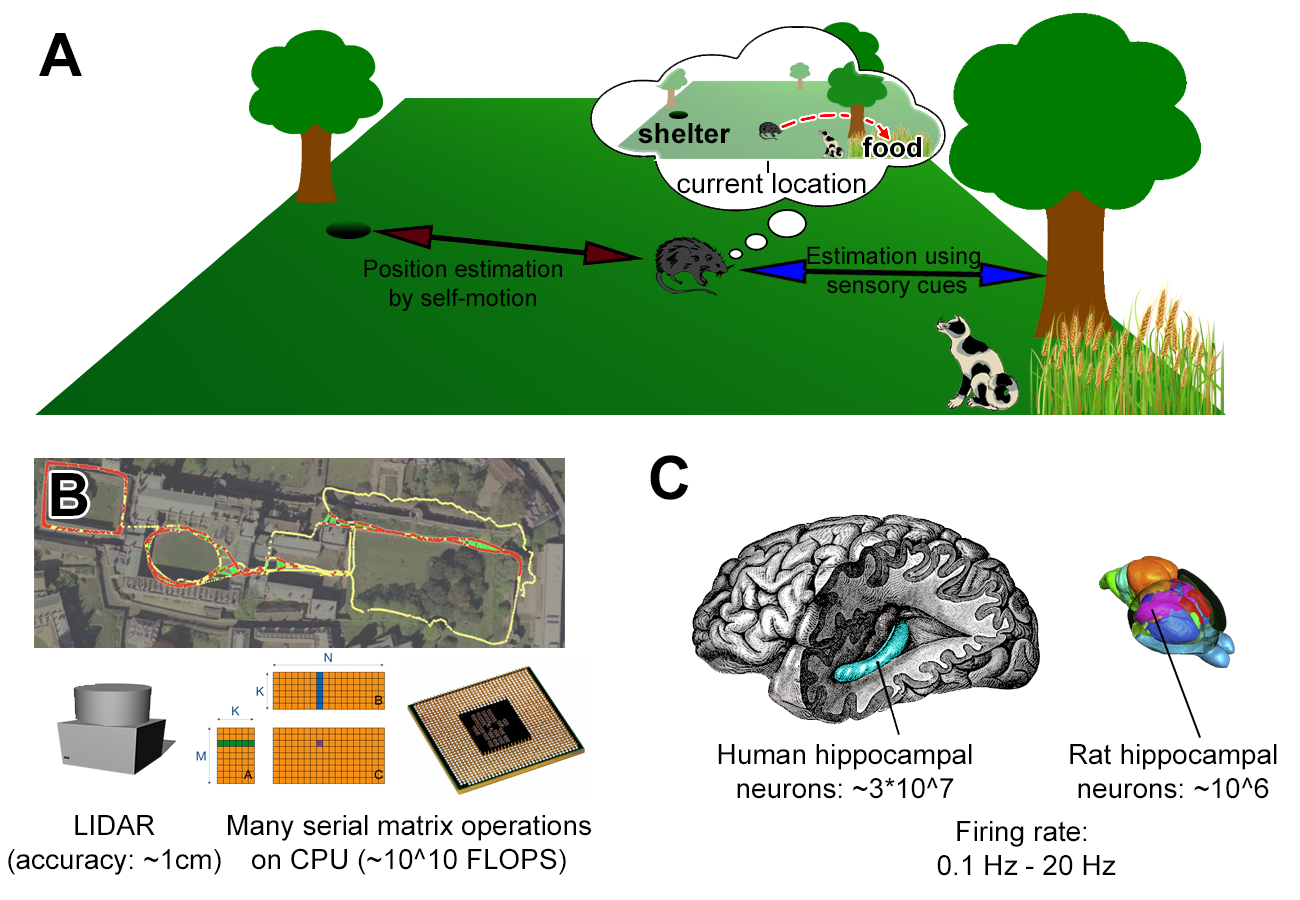
\includegraphics[width=\textwidth]{img/motivation}
	\caption[Motivation for proposing new computational cognitive models of spatial memory]{\textbf{Motivation for proposing new computational cognitive models of spatial memory}. A: Learning representations of the space around animals confers significant advantages, such as the ability to plan a detour out of sight (dashed red arrow) to reach a food source while avoiding danger in this example. In real environments, this task is made more difficult by the unreliability, errors and noise inherent in both the estimation of position by integrating self-motion and in estimated object distances (e.g. based on vision). Most existing cognitive models of spatial memory neglect these challenges. B: State of the art SLAM models in robotics are able to estimate locations and learn maps accurately, but rely on sensors and computations which are very different from biology - e.g. higher measurement accuracy using laser-based distance sensors (LIDAR), centralized control and coordination, and high number of serial operations per second - up to $10^{10}$ floating-point operations per second (FLOPS) needed for state of the art SLAM systems \citep{machado2013evaluation}. C: In contrast, the hippocampus - the major brain area involved in world-centered spatial representations - contains only a few million neurons, of which only a subset is active at a time, each firing only a few times per second \citep{rapp1996preserved,vsimic1997volume}; and relies on noisy, inaccurate sensory measurements. Although many models of spatial memory in brains exist, there is a lack of computational mechanisms which are both neurally and psychologically plausible, and can work in realistic environments and with noisy sensors. (Example SLAM data in Panel B from \citep{newman2011describing}, and 3D rat brain in Panel C from \citep{calabrese2013ontology}, with permission.)} 
	\label{fig:motivation}
\end{figure}

\section{Motivation}
\label{sec:intro:motivation}

Despite of this success and of the suitability of probabilistic models to deal with uncertain and noisy spatial information, there have been few attempts to use them for modelling spatial memory within cognitive modelling, the branch of cognitive science concerned with computationally simulating mental processes. There is a gap in the literature between probabilistic spatial models in robotics (called Simultaneous Localization and Mapping or SLAM) \citep{thrun2008simultaneous}, which are capable of dealing with real-world noise, uncertainty, and complexity to some extent, but are cognitively implausible\footnote{In our usage of the terms, a computational model is `psychologically plausible' (or `cognitively plausible') to the extent that it is consistent with psychological findings and can accurately reproduce psychology data, i.e. behaviours. Analogously, it is `biologically plausible' (or `neurally plausible') to the extent that it is consistent with neuroscience and can reproduce neural data, e.g. single-cell recordings or brain imaging results.}, and between computational cognitive models of spatial memory, which are designed to model biological spatial cognition, but cannot deal with all of these challenges, and are thus confined to simplistic simulations (see Chapter \ref{cha:nnreview} for a review). 

%There is also a dearth of models of \textit{how} neurons could be able to perform Bayesian inference to improve spatial representations, and of evidence on a neuronal level (as opposed to behavioural) that they can. 

In addition, although spatial representations in humans have been argued early to be hierarchical \citep{hirtle1985evidence, mcnamara1989subjective, greenauer2010micro}, similarly to some robotic implementations having to deal with large, complex environments \citep{kuipers2000spatial, wurm2010octomap}, it is not known how (by which process) these hierarchical spatial maps might be structured. Although many computational models of spatial memory running in simplified environments exist, there is a lack of biologically and psychologically plausible `algorithms' serving as models of human cognitive computations related to spatial information processing which can function in realistic, uncertain, complex environments.

The deprioritization of the problems of uncertainty and noise in favour of tractably modelling other human cognitive mechanisms is also pronounced in cognitive architectures, which try to account for a large number of mental processes in a unified, comprehensive, systems-level model (as opposed to computational cognitive models, which usually focus on a single phenomenon). In their overview of the field, \cite{langley2009cognitive} argue that \textit{`` we should attempt to unify many findings into a single theoretical framework, then proceed to test and refine that theory''}, supporting the arguments of \cite{newell1973you} that \textit{``you can't play 20 questions with nature and win''}, highlighting the importance of systems-level research in the cognitive sciences. Although a few such cognitive architectures do model spatial mechanisms in navigation space \citep{harrison2003act,schultheis2011casimir,sun2004top}, they all run in simple, noise-free environments. According to a comparative table of cognitive architectures \citep{samsonovich2011comparative} available in updated form online\footnote{http://bicasociety.org/cogarch/architectures.htm}, there is currently no cognitive architecture implementing both Bayesian update and an empirically validated, psychologically plausible `cognitive map' at the same time.
%\footnote{CogPrime \citep{goertzel2013cogprime} claims to implement both Bayesian update and cognitive maps, but neither of these mechanisms have been evaluated against human data, or indeed claim to be modelling human cognitive phenomena at all. Instead, CogPrime aims for artificial general intelligence, as opposed to closely adhering to human cognition.}.

\clearpage

The present work was motivated by these gaps in the literature, and aims to take computational cognitive models of navigation-scale\footnote{Human cognition needs to keep track of the space of navigation as well as the spaces immediately around the body (e.g. reachable objects) and of the body (e.g. body-part configurations). Although uncertainty and noise play are important in the latter two spaces as well, we will confine ourselves to navigation-scale spatial mechanisms in this work.} spatial memory one step closer to modelling behaviour in realistic environments, such as high-fidelity robotic simulations or physical environments. It aims to do so by means of proposing probabilistic mechanisms of spatial cognition which are implementable in brains and can reproduce behaviour data, and by computationally implementing these mechanisms, in the form of cognitive models and within an existing cognitive architecture. Situated within the computational sub-fields of cognitive science (cognitive modelling and cognitive architectures), the goal of this work is to contribute to the understanding of information processing in human cognition. As such, although it is computational in nature, the extent of its success is determined by its ability to predict and explain the kinds of behaviour data it is intended to model, as well as its consistency with established findings in psychology and neuroscience. It is not aiming for performance, or accuracy of learned spatial representations (these are the domains of robotics), or for maximizing neurobiological fidelity at the cellular level or below. Although building on neuroscientific evidence, our concern is modelling spatial information processing on Marr's algorithmic level of analysis \citep{marr1976understanding, marr1977understanding}, as opposed to e.g. biological neural networks - see Table \ref{tbl:marr} -, with a single exception. 

\begin{table*}[h]
	\centering
	{\renewcommand{\arraystretch}{1.2}
		\begin{tabu}{c|c|c}
			$\downarrow$ {Level of analysis} & {Description} & {In this work}\\ \tabucline[3pt]{-}
			1. Computational & \begin{tabular}[c]{@{}c@{}} What problem(s) does the \\ system solve, and why? \end{tabular} & \begin{tabular}[c]{@{}c@{}} Localization,\\ Map error correction, \\ Map structuring \end{tabular} \\\hline
			\begin{tabular}[c]{@{}c@{}} \textbf{2. Algorithmic/} \\ \textbf{Representational} \end{tabular} & \begin{tabular}[c]{@{}c@{}} How might it solve them? (Using\\ what representations and processes?) \end{tabular} & \begin{tabular}[c]{@{}c@{}} Cognitive models \\ of spatial memory \end{tabular} \\\hline
			3. Implementation & How is it implemented physically? & \begin{tabular}[c]{@{}c@{}} Place, grid,  head- \\ direction, border cells, \\ ... \citep{hartley2014space} \end{tabular} \\
		\end{tabu}
	}
	\caption[Investigating spatial mechanisms on Marr's (1976) levels of analysis]{\textbf{Investigating spatial mechanisms on Marr's (1976) levels of analysis}. The present work is mostly concerned with the second level.}
	\label{tbl:marr}
\end{table*}
%\begin{tabular}[c]{@{}c@{}} Approximately Bayes- \\optimal integration\\of information \end{tabular}

Unlike the rest of our work, we have investigated the plausibility of Bayesian spatial cue integration both on Marr's algorithmic (Chapter \ref{cha:lida}) and implementation level (Chapter \ref{cha:bayespc}), in order to maintain the desirable criteria of both psychological and neural plausibility for our other models. Although this mechanism has been empirically substantiated on a behavioural level before \citep{cheng2007bayesian, nardini2008development}, its neural implementation has remained in doubt, with current mechanistic models of Bayesian inference in brains making assumptions not fully consistent with the anatomy or activity of the hippocampal complex (the major brain areas representing world-centered spatial information) - see next Section. This doubt of biological implementability has motivated our investigation of single-cell electrophysiological data (acquired outside this PhD) to provide the first evidence for Bayesian updating in the hippocampus on a neuronal level, and our proposal of a plausible mechanism for implementing it. This evidence, presented in Chapter \ref{cha:bayespc}, affords a degree of biological plausibility to the models utilizing Bayesian mechanisms in the rest of our work (which is concerned with processes on the algorithmic/representational level).

%especially if behavioural evidence is inconclusive or insufficient to constrain the space of possible models to a concrete implementation

\section{Probabilistic models of space in brains and minds}
\label{sec:intro:uncertaintybrain} 

Although the focus of most of this work is on the computational modelling of behaviour data, we would like the employed mechanisms to be plausibly implementable in the parts of the brain they functionally correspond to. Apart from the lack of neuronal-level evidence that the hippocampal complex may perform Bayesian inference or even represent uncertainty, the possibility of the implementation of such a mechanism given the anatomical and electrophysiological constraints of this network of brain cells is also unclear. 

Below, we briefly review probabilistic neural spatial models which have been proposed in the literature (Chapter \ref{cha:nnreview} provides more general review of computational cognitive models of spatial memory). We start with normative models of dealing with spatial uncertainty, which derive optimal solutions to the problem a system might be solving (Marr's computational level). We then continue describing mechanistic (implementation level) models which might facilitate these, and their consistency with what is known about the hippocampal complex. More extensive reviews of Bayesian models in brains can be found in \citep{pouget2013probabilistic, vilares2011bayesian}. There is currently little experimental support for any of the proposed neural uncertainty representations. % \citep{pouget2013probabilistic}. 

%In addition to a large number of non-probabilistic computational cognitive models focusing on accounting for specific mechanisms of spatial cognition (see Chapter \ref{cha:nnreview} for a review), a few authors have suggested probabilistic mechanisms the brain might employ which can be used to model spatial cognition.

Models of probabilistic estimation of spatial information have been pioneered by \citep{bousquet1997hippocampus}, who suggested to use a Kalman filter to model localization in the hippocampus. A Kalman filter is a dynamic Bayesian inference algorithm for estimating the values of unknown, not directly observable variables (such as location) from noisy observations, yielding statistically optimal estimates if the noise is normally distributed \citep{kalman1960new}. \citet{macneilage2008computational} also put forth arguments for dynamic Bayesian inference as a model of spatial orientation. They mention both Kalman filters and particle filtering (a related Bayesian filtering algorithm using samples instead of parameters to represent probability distributions), but leave the question of their neural implementation open. Particle filter-based models of localization on the algorithmic level have been suggested by \citep{fox2010hippocampus, cheung2012maintaining}. \citet{osborn2010kalman} went beyond localization, suggesting a Kalman filtering approach to also account for localizing objects in the environment. Recently, \citet{penny2013forward} argued that if one presupposes the existence of `observation' and `dynamic' models\footnote{Observation models and dynamic models are mathematical functions mapping from true states to observed states, and from pre-motion to post-motion states, respectively.}, required by Kalman filters, one might as well extend the inference to also use them for model selection (`which environment am I in?'), motor planning (`how do I get to place X?'), and to construct sensory imagery (`what does place X look like?') in addition to localization. They have combined these functions in a single probabilistic model, and argued that it is consistent with findings of pattern replay in the brain. An even more general probabilistic formulation based on dynamic Bayesian inference is the Free-Energy Principle \citep{friston2006free}, which aspires to provide a unified theory of brain function, and has been argued to be consistent with aspects of hippocampal processing \citep{friston2011action}.

Despite their considerable theoretical elegance, the above-mentioned models do not provide a final and complete answer to the motivating question of this thesis (Section \ref{sec:intro:motivation}), which can be summarized as: `how does biological cognition learn representations of navigation space from noisy sensors in an uncertain world?', for two reasons. First, none of them try to reproduce or show quantitative consistence with either behavioural or neural data concerning spatial cognition (although qualitative consistence with anatomical and neural findings is pointed out by the authors). Although these models provide explanations, their predictions regarding spatial processing have not been quantitatively evaluated.

Second, in addition to the lack of quantitative validation, their neural implementation is not known, and far from straightforward. For example, implementing the kinds of large matrix inversions and multiplications required by Kalman filters \citep{kalman1960new} is easy on a computer, with centrally coordinated, serial, `fast' computations, but difficult with the kind of distributed, parallel, `slow' (on the level of single neurons, which only spike up to a few dozen times per second) computation performed by the brain. In the domain of world-centered, navigation-scale spatial mechanisms, any suggested neural implementation has to conform with not only the limitations imposed by biological neural networks, but also with the specific connectivity and activity observed in the hippocampal complex, in order to be considered biologically plausible.

In addition to such normative models, a number of mechanistic (implementation-level) models of how uncertainty and inference could be implemented in brains have also been proposed. They can be roughly grouped into three categories - see \citep{pouget2013probabilistic, vilares2011bayesian} for reviews. We briefly summarize these groups below, together with their consistency with what is known about the hippocampus. 
%, which would be suitable for spatial localization or map learning in the face of uncertainty, together with the main reason we chose not to adopt that mechanism in this work. Detailed arguments regarding these reasons can be found in Appendix A.

% free-form approximations do not scale

% no electrophysiological or psychophysical evidence to suggest that the brain can encode multimodal approximations:

\begin{itemize}

\item Probabilistic population codes (PPC) \citep{ma2006bayesian} encode probability distributions in the logarithmic domain by means of a set of coefficients of corresponding exponential basis functions, each coefficient encoded by the activity (spike count) of a neuron. They assume neural variability is independent and Poisson-distributed. However, hippocampal neurons exhibit more variability than a Poisson process \citep{fenton1998place, barbieri2001construction}. Also, if Bayesian inference were implemented in the hippocampus via a PPC, the encoded probability distributions would strongly depend on the firing rate of hippocampal neurons: increased firing rates should mean decreased levels of uncertainty. But empirically, this is not the case - for example, firing rates increase with movement speed \citep{maurer2005self}, which would mean the lowest uncertainties when running fastest (however, faster movements are harder to control and should thus lead to higher uncertainty). 

\item Instead of an encoding in the logarithmic domain, codes in which firing rates are proportional to probabilities have also been proposed, e.g. by \citet{koechlin1999bayesian, barber2003neural}. The problem with their implementation in hippocampal neurons is that the firing rates of these neurons are also influenced by factors unrelated to probability, such as where the animal is headed \citep{ferbinteanu2003prospective} or trial dependent features \citep{allen2012hippocampal}, and can change substantially if either the shape or colour of an environment is altered \citep{leutgeb2005independent}. These influences would strongly interfere with the outcome of the Bayesian inference, if it were implemented in a code that directly utilizes firing rates.

\item Sampling-based codes represent probability distributions with a set of samples drawn from them \citep{fiser2010statistically}. They are asymptotically correct with infinitely many samples, and approximations otherwise. Apart from being able to represent complex, multi-modal distributions, not having to rely on any fixed-form parametrization such as Gaussians, this also allows reducing their accuracy and computational demands by restricting the number of samples used. This property has been used e.g. by \citep{shi2010exemplar} to explain the deviations from the statistical optimum in an exemplar model of a reproduction task. It is difficult to make a general statement as to the implementability of this class of models in the hippocampal complex, as there is a wide variety of suggested concrete neural implementations in non-spatial domains (\citet{sanborn2015types} provides a review), and some applied to navigation space, e.g. \citep{fox2010hippocampus, cheung2012maintaining}. None of them have been quantitatively validated by neural (electrophysiological) measurements, although most of them are supported by behavioural observations. 

%\item \citet{deneve2007optimal} [attractor networks] %  rather than coding for the log probability that a feature is present, neurons code for the log probability that a feature takes on a particular value
%\item \citet{ma2006bayesian} [PPC]
%\item \citet{fiser2010statistically} [sampling]
%\item \citet{friston2011action} [FEP]

\end{itemize}

How the brain might encode and utilize uncertainty is still an open question \citep{pouget2013probabilistic}, but based on the observations regarding the hippocampus outlined above, we argue that a sampling-based code is most suitable in this brain area; in terms of violating as few empirical observations as possible. We will provide electrophysiological evidence of Bayesian inference from single neurons, and propose a possible sampling-based mechanism, in Chapter \ref{cha:bayespc} (and in more detail in Appendix TODO).


%bousquet et al kalman filter

%fox prescott

%penny pioneered ... extend this line of research... difficult to actually implement, as EKF O(n^2)

%Khamassi and Humphries [18] argue that, due to the shared underlying neuroanatomy, spatial navigation strategies that were previously described as being either place-driven or cue- driven are better thought of as being model-based versus model- free. Daw et al. [15] propose that arbitration between model-based and model-free controllers is based on the relative uncertainty of the decisions

% friston action understanding

% make things as simple as possible, but not simpler

% implicitly - RatSLAM

\section{Hypotheses}
\label{sec:intro:hypotheses}

To achieve goals in a spatially extended, realistic environment, at a minimum, an agent (e.g. a biological agent such as an animal, or an artificial agent such as a robot) must be able to 1) move, and keep track of its movements, 2) sense, and interpret its sensations, 3) represent spatial locations in its environment, e.g. of itself and its goal, 4) update these representations when changes occur in the environment, and 5) utilize these representations to achieve its goals (e.g. navigate to its goal location, avoiding dangers). Extensive work on all levels of analysis has been carried out for 1)-3), with the most recent Nobel prize in physiology or medicine awarded on the topic of 3) to John O'Keefe, May-Britt Moser and Edvard I Moser for the discovery of \textit{`cells that constitute a positioning system in the brain'} \citep{burgess2014nobel}. Specifically, it was awarded for the discovery of `place cells' in the hippocampus (which show increased firing in a specific area in the environment, called its `place field'), and of `grid cells' which show a regular, grid-like firing pattern (see Chapter \ref{cha:nnreview} below). 

We have argued above that despite of the variety of existing models regarding 4)+5), new computational models are needed to move towards biological and psychological plausibility as well as real-world capability at the same time (since biological cognition has been shaped by the constraints and challenges of the real world, these should not be neglected in models of cognition). In particular, in accordance with the `Bayesian brain' \citep{knill2004bayesian} and `Bayesian cognition' \citep{chater2010bayesian} paradigms, we have suggested approximate Bayesian inference to be a well-suited mechanism for tackling these challenges. Models on Marr's algorithmic (and implementation) level which utilize such a mechanism require a number of underlying assumptions, some of which can be stated and evaluated as hypotheses. 

We summarize major hypotheses in one place in Table \ref{tbl:hyp} below, and expand on them in the respective results chapters below. The first two concern the representation and manipulation of uncertainty in the hippocampus (required for maintaining approximately accurate location estimates despite noisy sensors and accumulating errors). Hypothesis 3 is needed since unless all remembered landmark locations are corrected at every moment (which would likely be intractable), a discrepancy between remembered and actual locations might arise when revisiting a location encountered previously (when traversing a `loop' in the environment). This discrepancy necessitates a backward correction of multiple recent self and landmark locations to maintain consistent representations. The last two are needed to formulate a computational mechanism of spatial representation structure. Structured, hierarchical representations provide clear computational advantages, such as increased speed and efficiency of retrieval search, and economical storage. However, although strong neural \citep{derdikman2010manifold} and behavioural \citep{hirtle1985evidence, mcnamara1989subjective, greenauer2010micro} evidence exists for such structure, underlying computational principles have remained largely unknown.

\newpage

\setlength\tabcolsep{4pt}
%\small
\begin{longtable}{|p{4.5cm}|p{4.5cm}|p{4.6cm}|}
	\hline
	\textbf{Hypothesis} & \textbf{Prediction} & \textbf{Empirical support} \\
	\hline
	
	1 Hippocampal place cells can perform approximate Bayesian inference & {Place field size depends on uncertainty (e.g. proximity of landmarks) in a} & {Place field sizes (recorded from hippocampal neurons of behaving rats) are cor-} \\ \cline{1-1} 
	2 Spatial uncertainty is represented as the size of place cell firing fields & Bayesian fashion & related with uncertainties predicted by a Bayesian model (Chapter \ref{cha:bayespc}) \\ \hline
	3 When revisiting a place, estimates of recently traversed locations and encountered landmarks are updated in an approx. Bayes-optimal fashion & After revisiting parts of an environment, place fields should shift, and recently active place cells should re-activate. Errors should conform to Bayesian predictions & Neural: none in this work, but place fields seem to shift after revisits \citep{mehta2000experience}, and recently active place cells do reactivate (`replay') \citep{carr2011hippocampal}. Behavioural: errors correlate with predictions (Chapter \ref{cha:lida}) \\ \hline 
	4 The structure of spatial representations arises from clustering & Landmarks which are co-represented (belong together) in participants' & Neural: none in this work. Behavioural: the probability of two landmarks being \\ \cline{1-1}
	5 This clustering mechanism operates on features including Euclidean distance, path distance, boundaries, visual and functional similarity & spatial memory should be closer in these features than those not belonging together & co-represented is strongly correlated with distances along these specific features. These distances allow prediction of participant representation structure (Chapter \ref{cha:structure}) \\
	
	\hline
	\captionsetup{width=\textwidth}
	\caption[Hypotheses of the models presented in this work]{\textbf{Hypotheses of the models presented in this work, and empirical support}. Place cell electrophysiological recording data was acquired outside this PhD. All other data has been collected by the author, unless otherwise specified.}
	\label{tbl:hyp}
\end{longtable}


\section{Outline and Contributions}
\label{sec:intro:outline}

This thesis is presented in the Alternative Format allowed by the University of Manchester presentation of theses policy \footnote{http://documents.manchester.ac.uk/DocuInfo.aspx?DocID=7420}, which allows incorporating sections in a format suitable for publication in peer-reviewed journals. We chose the alternative format to more easily accommodate already published work, to reduce risks of self-plagiarism,  and because of the largely self-contained nature of our individual results chapters. Thus, in what follows, the literature review (Chapter \ref{cha:nnreview}) and the three chapters (\ref{cha:bayespc}-\ref{cha:lida}) reporting the results, are copies of papers either accepted by or submitted to peer-reviewed journals. The following list summarizes these papers and the contributions\footnote{In all publications, Madl wrote the draft of the paper, developed the software, designed the experiments, recruited and tested the participants where applicable, and analysed the data. Corrections suggested by Chen, Montaldi, and Franklin were incorporated into the final drafts by Madl after discussions with these co-authors. All publications were supervised by Chen and Montaldi, with Chen mainly commenting on mathematical and computational issues, and Montaldi on psychological and neuroscientific issues.} therein:

\begin{itemize}
	\item Chapter \ref{cha:nnreview}: Madl T., Chen K., Montaldi D. \& Trappl R., 2015. Computational cognitive models of spatial memory in navigation space: A review. \textit{Neural Networks, 65, 18-43.}
	\\ Contributions: 1) a systematic review of representative cognitive models concerned with navigation-scale spatial memory, falling into symbolic, neural network, or cognitive architecture models, including a comparative table of the characteristics of these models.
	\item Chapter \ref{cha:bayespc}: Madl T., Franklin S., Chen K., Montaldi D. \& Trappl R., 2014. Bayesian Integration of Information in Hippocampal Place Cells. \textit{PLoS ONE 9(3), e89762}
	\\ Contributions: 2) first quantitative electrophysiological validation of the representation of spatial uncertainty in the brain, and of Bayesian integration of spatial information in the brain, in three different environments (using data acquired outside this PhD). 3) Formulation and empirical support for an inference mechanism based on coincidence detection (falling into the camp of sampling-based models of neural inference)
	\item Chapter \ref{cha:structure}: Madl T., Franklin S., Chen K., Trappl R. \& Montaldi D., submitted. Exploring the structure of spatial representations. \textit{Cognitive Processing}
	\\ Contributions: 4) behavioural evidence for clustering as the normative principle underlying spatial representation structure, and 5) the first computational model of navigation-scale spatial representation structure on the individual level (able to predict this structure in participants' long-term spatial memory from the geospatial properties of an environment)
	\item Chapter \ref{cha:lida}: Madl T, Franklin S, Chen K, Montaldi D \& Trappl R, submitted. Towards real-world capable spatial memory in the LIDA\footnote{LIDA stands for Learning Intelligent Distribution Agent, and is reviewed in a paper co-authored during this PhD but not included in this thesis: \citep{franklin2013lida}} cognitive architecture. \textit{Biologically Inspired Cognitive Architectures}
	\\ Contributions: 6) integration of three spatial mechanisms capable of dealing with uncertainty and noise into a comprehensive cognitive architecture (localization, map structuring, map correction), and 7) embodying this architecture on a robot, allowing demonstration of the model functionality in a realistic robotic simulator. 8) proposal of a biologically plausible mechanism for correcting errors in learned maps when revisiting an already known place (the `loop closure' problem, well known in robotics, but neglected in cognitive science), and evaluation against behaviour data regarding cognitive map accuracy in human subjects.
\end{itemize}

The model best accounting for spatial memory structure presented in Chapter \ref{cha:structure} also constitutes a novel kind of metric learning in machine learning, based on the idea of learning a similarity function in the space of absolute pairwise differences (as opposed to e.g. a Mahalanobis distance function). Although proposed before in a similar form for person re-identification in the computer vision community \citep{zheng2011person}, the insight that this space contains neglected information which can be utilized to improve performance in general (not just on image data), and the general formulation allowing arbitrary constituent models for learning a metric in this space, are a novel contribution (9). Since it is too far from the topic of this thesis, metric learning in absolute pairwise difference space is only described briefly (to the extent required to model cognitive map structure) in Chapter \ref{cha:structure}. Applications and results on other kinds of data, with other constituent models, and in a semi-supervised setting, and are briefly summarized in Appendix TODO.

After presenting the mentioned papers constituting the literature review and results chapters, we present an analysis of the methods employed during this research in Chapter \ref{cha:methods}. We continue to discuss the implications of our results and the neural implementability of the mechanisms for which a concrete implementation has not already been presented in the results in Chapter \ref{cha:discussion}. We conclude in Chapter \ref{cha:conclusion} with a conclusion and an outline of potential future work opened up by this research. 

We note that the line of criticism mentioned regarding the neural implementability of the high-level probabilistic models of localization in the previous section also apply to our proposed mechanism of cognitive map structuring (Chapter \ref{cha:structure}). Although it is intended to be a cognitive and not a neural model, we have argued that consistency with the underlying neuroscience can and should play a role in constraining the space of possible models, and evaluating models, even on the algorithmic level. But the map structuring mechanism in Chapter \ref{cha:structure} is, to our knowledge, the first formal model of the observed structure in cognitive maps, both on Marr's computational and algorithmic levels. We did not have the time and resources to extend it down to include a plausible neural implementation within this PhD.

Finally, work done during this PhD has contributed to two more publications which are not included in this thesis (the former because it is a conference paper, whereas University policy requires alternative format theses to contain journal papers instead; and the latter because it does not fit in well with the main topic):

\nocite{madl2013spatial, franklin2013lida}

\begin{itemize}
	\item Madl T., Franklin S., Chen K. \& Trappl R., 2013. Spatial working memory in the LIDA cognitive architecture. \textit{Proceedings of the International Conference on Cognitive Modelling (2013), pp. 384-389}
	\item Franklin S., Madl T., D'Mello, S., Snaider, J., 2014. LIDA: A Systems-level Architecture for Cognition, Emotion, and Learning. \textit{IEEE Transactions on Autonomous Mental Development 6(1), pp. 19-41}
\end{itemize}

\chapter{Computational Methods}
\label{cha:methods}

As mentioned in the Introduction, the goal of this thesis is bringing computational cognitive models closer to being able to function in realistic environments under conditions of uncertainty, by proposing probabilistic models of spatial cognition which are implementable in brains. Probabilistic models have become successful and widespread in domains requiring the representation and manipulation of uncertainty, including artificial intelligence \citep{russell2009ai}, robotics \citep{thrun2005probabilistic}, and machine learning \citep{bishop2006pattern}. They have also been successfully employed in cognitive modelling  \citep{chater2010bayesian} and in neuroscience \citep{knill2004bayesian} - although there is little empirical evidence for particular neural implementations of probabilistic mechanisms as of yet \citep{griffiths2008bayesian, vilares2011bayesian, pouget2013probabilistic}. 

This section briefly reviews the computational methods employed in this thesis. Figure \ref{fig:methods} shows an overview over all employed methods, and the way they are utilized to support the mechanisms, algorithms, and cognitive models presented below. Figure \ref{fig:neurimpl} connects these computational mechanisms to their suggested implementation in brains (arguments and evidence for the neuroscientific plausibility of Bayesian localization are presented in Chapter \ref{cha:bayespc}). 

\begin{figure}[h]
	\centering
	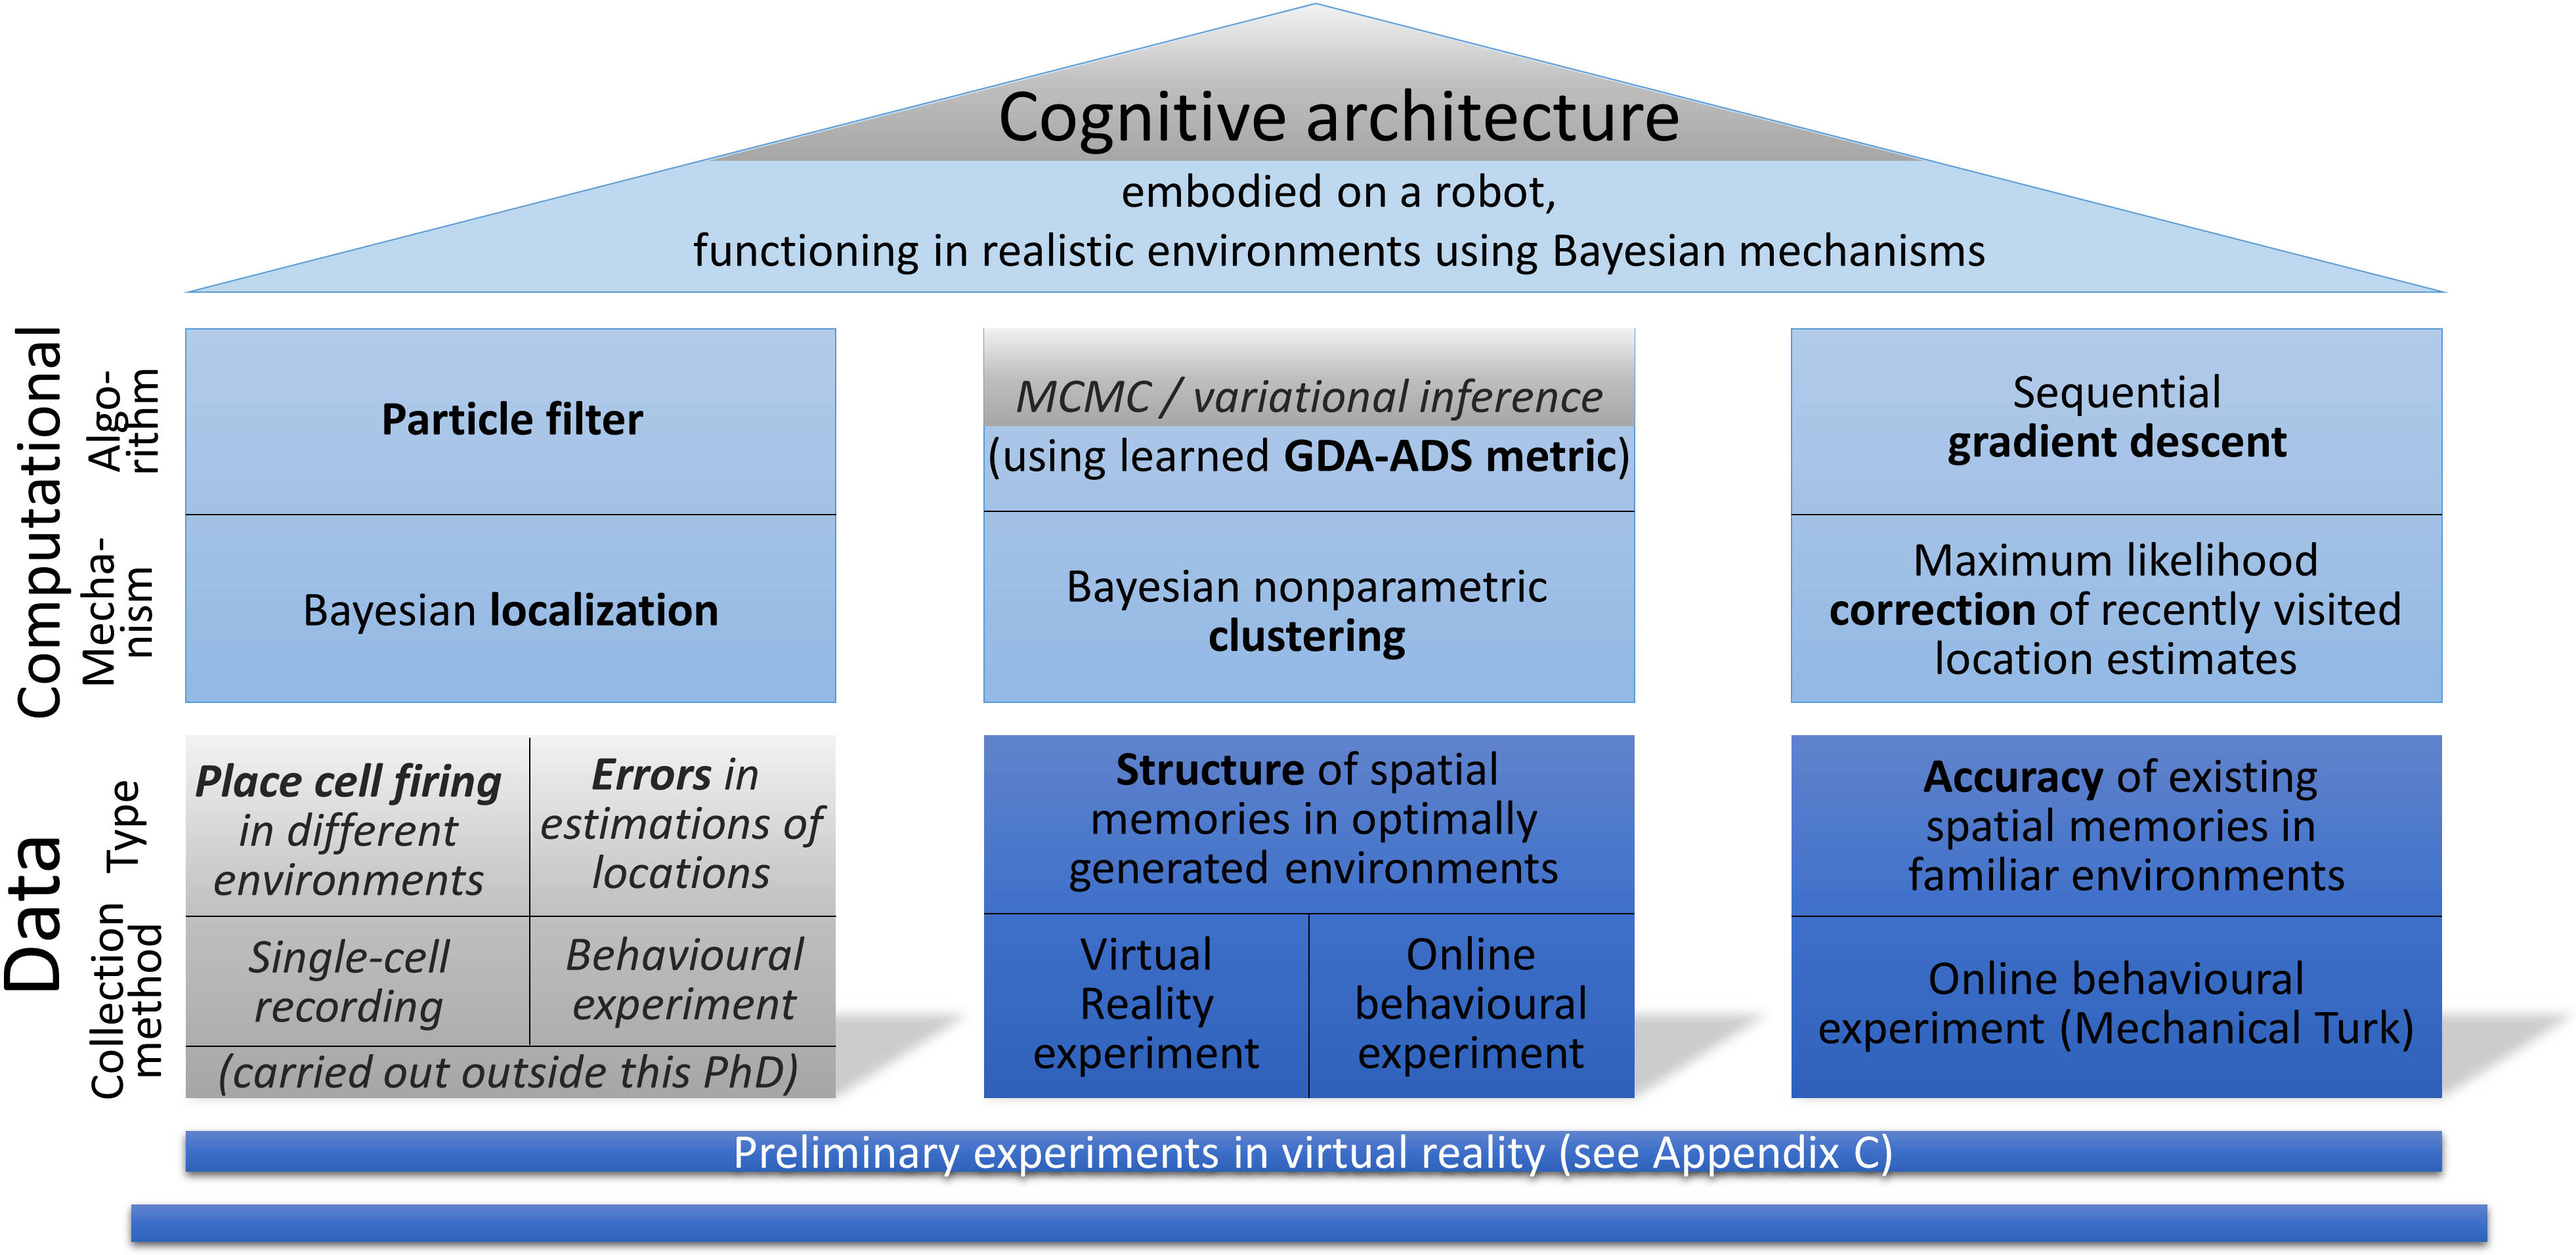
\includegraphics[width=\textwidth]{img/methodsfigure2}
	\caption[Overview of how the methods in this thesis help support real-world capable models of cognition]{\textbf{Overview of how the methods in this thesis help support real-world capable models of cognition,} roughly divided into empirical methods (bottom half) and computational methods (top half). Gray boxes contain data/code used to substantiate or implement some models, but not gathered/implemented by us.} 
	\label{fig:methods}
\end{figure}

To be able to plan novel routes in pursuit of its goals, an agent (whether biological or artificial), at a minimum, needs to be able to localize itself, its goal, and possible obstacles; and needs to do so in the face of a noisy and inaccurate sensory apparatus. From a probabilistic perspective, this localization problem can be described as a Bayesian network (see Figure \ref{fig:neurimpl}B). In order to avoid having to perform calculations over every location ever visited, and every landmark ever observed, as done in many robotics solutions \citep{durrant2006simultaneous,bailey2006simultaneous}, we split it into sub-problems. 

Specifically, an approximate solution of this problem can be split into Bayesian cue integration for integrating noisy observations into a location estimate (Section \ref{sec:bayescue}), Bayesian localization for maintaining this location estimate through time (Section \ref{sec:bayesloc}), and maximum likelihood-based correction for fixing the most recent location estimates when revisiting a location (Section \ref{sec:bayescorr}). We suggest a rejection sampling-based algorithm for the former two, implementable through coincidence detection in hippocampal place cells (Chapter \ref{cha:bayespc}), and a gradient descent-based solution for the latter, implementable by reverse replay in the hippocampus (Chapter \ref{cha:lida}). We will present empirical evidence for these claims in those chapters, both from single-neuron recordings in live animals (collected outside this PhD) and from behavioural experiments performed online with participants recruited from Amazon's Mechanical Turk\footnote{https://www.mturk.com}.

These mechanisms help inferring spatial locations in the environment from noisy observations, in a neurally and psychologically plausible fashion, as we will argue below. However, in a system operating under limited time and resources, these locations also need to be stored efficiently, such that they can be rapidly accessed. Hierarchical representations facilitate such desirable properties, and have been argued to be prevalent in human cognition \citep{cohen2000hierarchical, gobet2001chunking}. There is strong evidence

\nocite{deshmukh2013}

\begin{figure}[h]
	\centering
	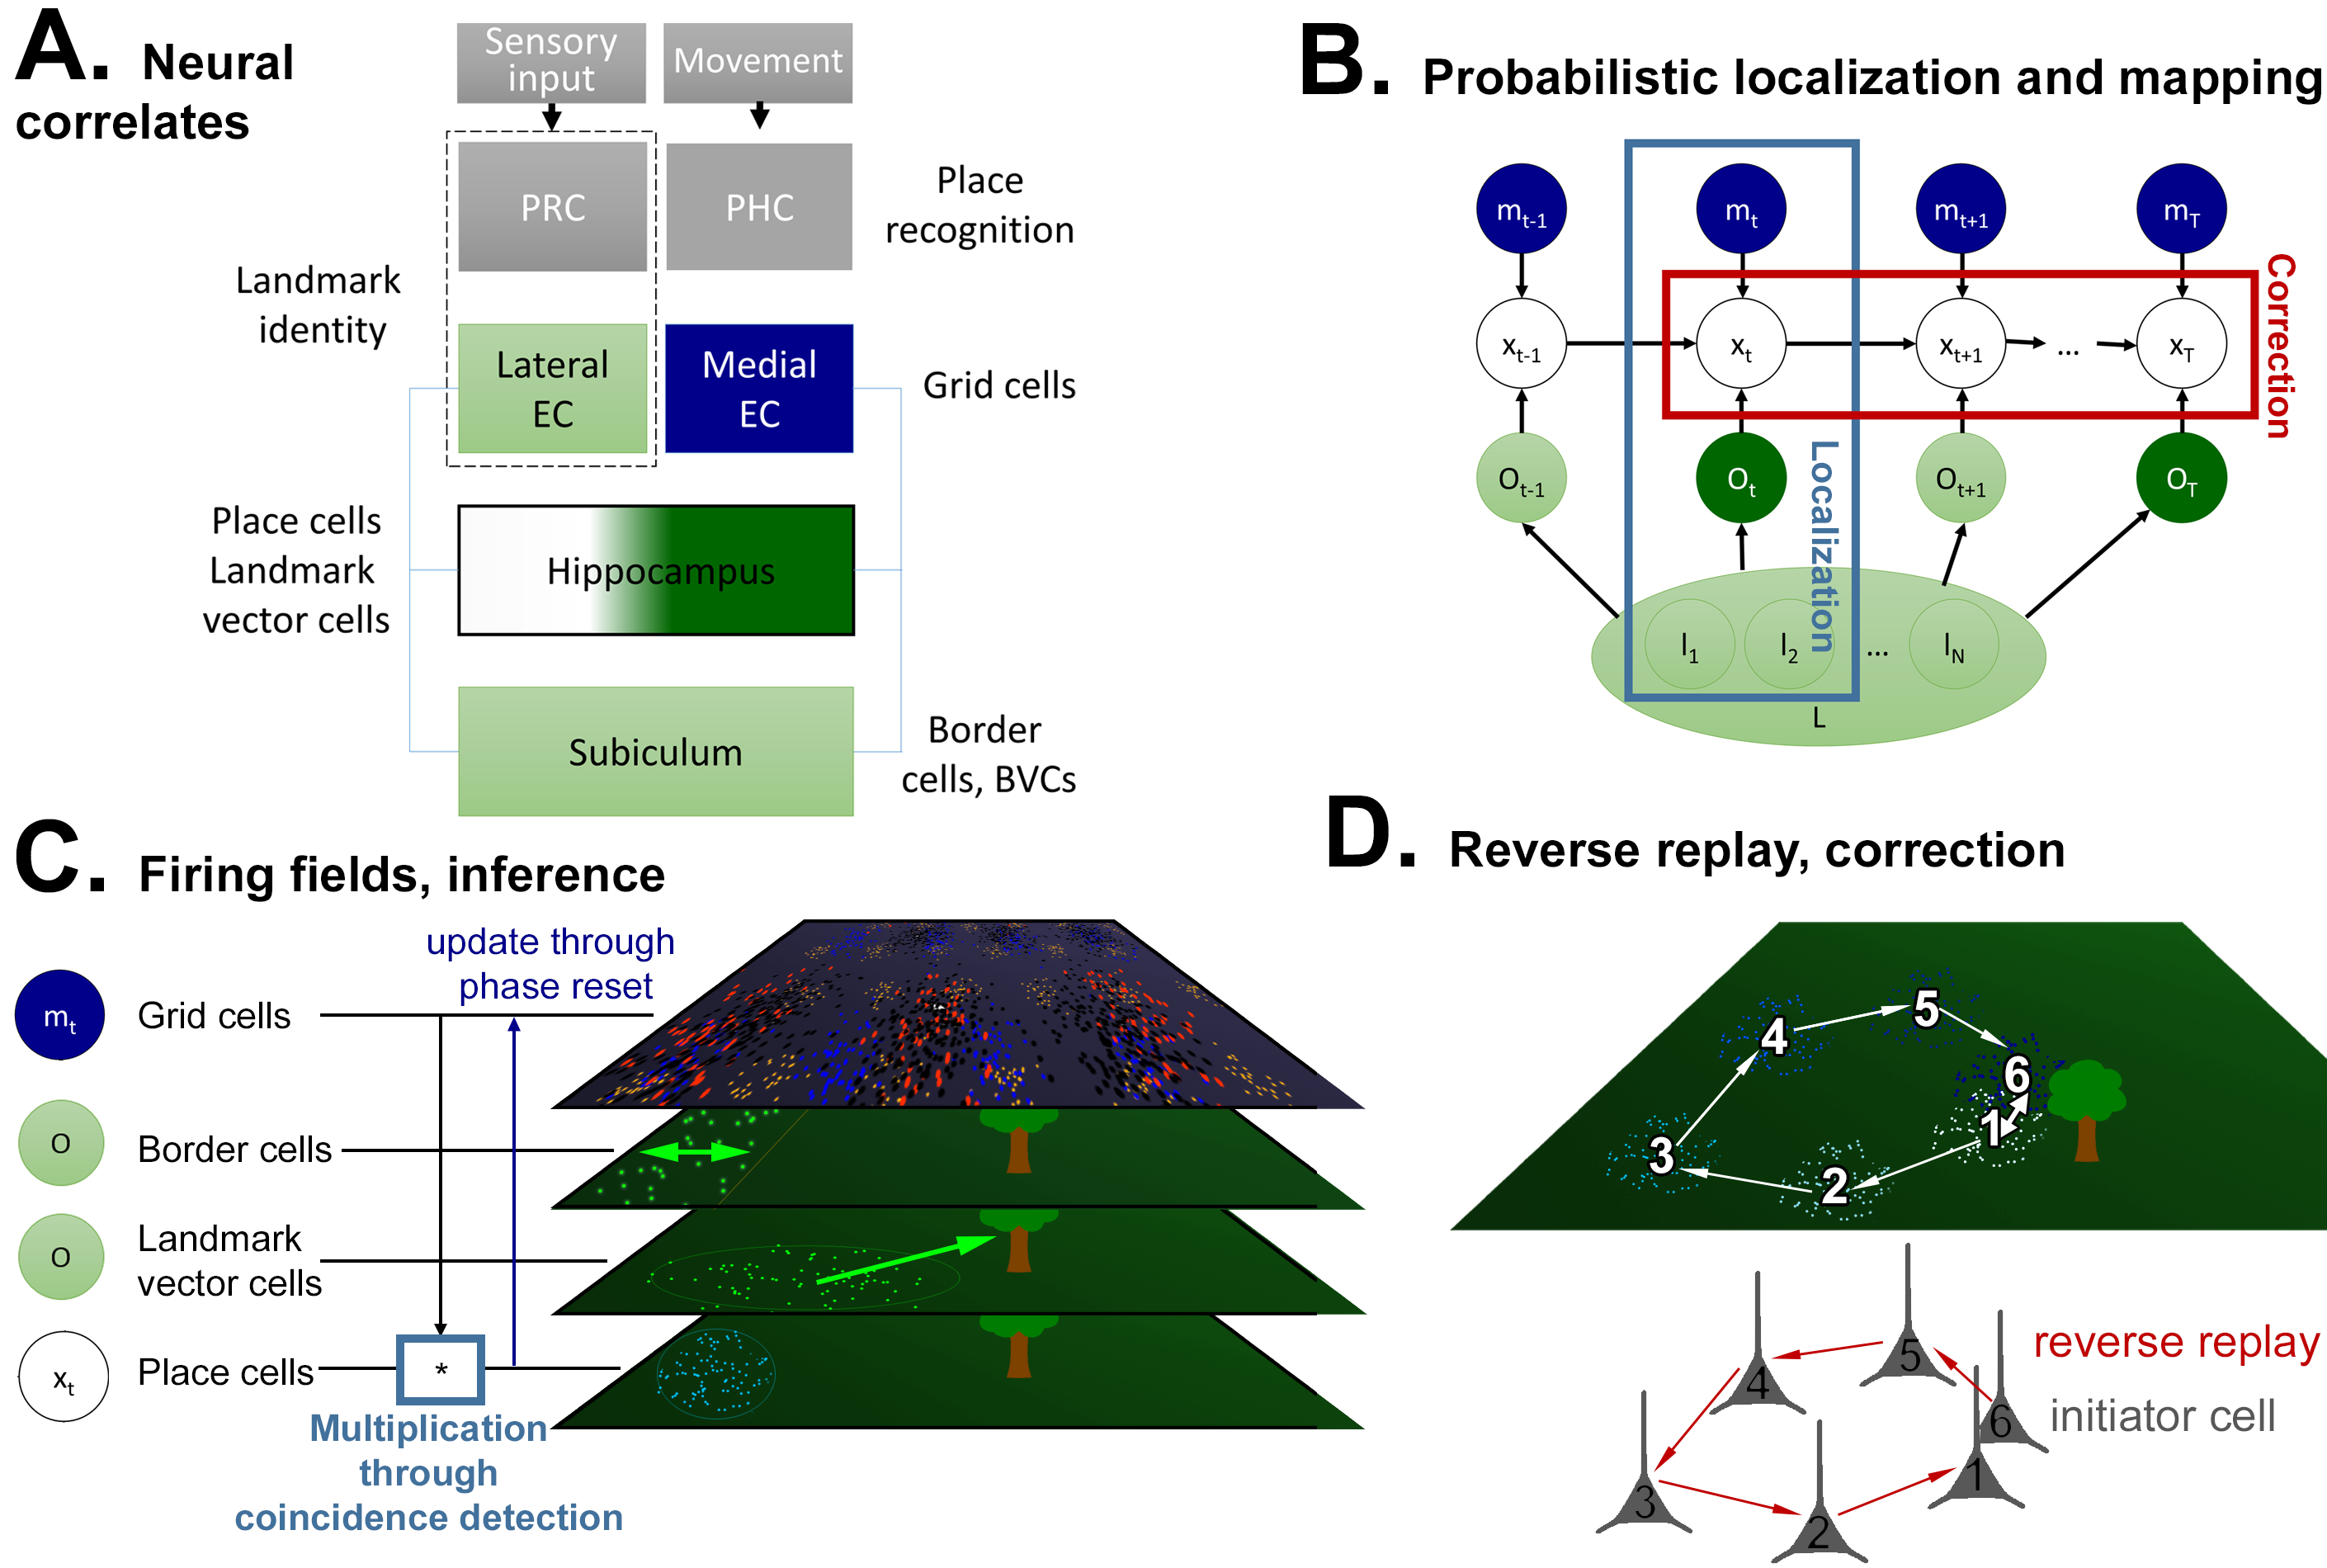
\includegraphics[width=\textwidth]{img/neurimpl3}
	\caption[Probabilistic spatial localization and mapping implementable by brains]{\textbf{Probabilistic spatial localization and mapping implementable by brains}. A: Neural correlates of localization. PRC: Perirhinal cortex, PHC: Parahippocampal cortex, EC: Entorhinal cortex (see Chapter \ref{cha:nnreview} for details; and (Deshmukh et al., 2013) for evidence of landmark vector cells). B: Probabilistic graphical model of the simultaneous localization and mapping problem \citep{thrun2008simultaneous}. Instead of capturing all correlations introduced through the landmarks, which requires vast computational resources, our model separately solves Bayesian localization with only local landmarks, and map correction (`pose optimization' in SLAM) with only loop closure constraints. See Chapter \ref{cha:methods} for notation and details. C: Illustration of firing fields during localization. Coloured dots represent spikes of the respective cells at specific locations. Path integration (grid cells) and boundary and landmark information (border cells, landmark vector cells) is integrated in place cells, using coincidence detection (rejection sampling) to obtain a near-optimal location estimate. This new estimate is used to update grid cell representations via phase reset to combat accumulating path integration errors (see Chapter \ref{cha:bayespc}). D: Illustration of a small loop (firing fields 1-6) which can be corrected upon recognizing the same landmark at positions 1 and 6 via reverse replay, by reactivating place cells 6-1 and shifting their place fields proportionally (see Chapter \ref{cha:lida}).
	} 
	\label{fig:neurimpl}
\end{figure}

\clearpage

\noindent that human spatial memories in particular are organized hierarchically \citep{hirtle1985evidence, mcnamara1989subjective, greenauer2010micro}, but the principles underlying these structures have not been known. We suggest a Bayesian nonparametric clustering model for structuring object representations under a subject-specific metric to account for human cognitive map structure (Section \ref{sec:bayesmap}), and present empirical evidence for this claim gathered from virtual reality and real world environments in Chapter \ref{cha:structure}.




These probabilistic models for inferring self locations and object locations and structuring their representations constitute the pillars of a cognitive software agent able to function in a realistic robotic simulator, which provides the same interfaces as a real robot (and would allow this agent to run on a real robot without modifications to its code) \citep{rusu2007extending}. We have implemented this agent within the LIDA (Learning Intelligent Distribution Agent) cognitive architecture, extending it with a spatial memory module and the described probabilistic models, integrating them with the other mechanisms already implemented in LIDA. Describing LIDA is outside the scope of this thesis, but see the review by \cite{franklin2013lida}, co-authored during this PhD.

Figure \ref{fig:neurimpl} above provides an overview over how the Bayesian mechanisms summarized above may be implemented in spatially relevant brain areas, and pointers to the parts of this thesis substantiating these connections; lending credence to our claim that our probabilistic models are neurally plausible (implementable in brains). Chapter \ref{cha:bayespc} provides the first neural-level evidence for Bayesian inference in these brain areas. 
%The rest of this thesis is concerned with showing that these mechanisms are useful in modelling human behaviour, and in making cognitive models work on robots.

%More specific and detailed descriptions of each method, including the empirical methods used to gather data for testing hypotheses for which no existing datasets could be found, are described in the respective result chapters. Chapter \ref{cha:bayespc} contains descriptions of the place cell firing data and its computational modelling, and Chapter \ref{cha:structure} the collection of data regarding spatial memory structure and accuracy data and its modelling. Chapter \ref{cha:lida} integrates the models in the same architecture, and interfaces them to a robotic simulator. 

%Describing the details of the LIDA (Learning Intelligent Distribution Agent) cognitive architecture \citep{franklin2013lida}, within which these cognitively plausible Bayesian mechanisms have been computationally realized, is outside the scope of this thesis.


\section{Probabilistic modelling}

Probabilistic models use probability distributions to represent quantities and the uncertainties associated with them, utilizing probability theory to manipulate these distributions \citep{ghahramani2015probabilistic}. Two basic rules provide the foundation, and together yield Bayes' theorem, which underlies Bayesian modelling. The \textit{sum rule} takes the form

\begin{equation}
\label{sumrule}
p(Y) = \sum_{X} p(Y, X),
\end{equation}

where $p(X,Y)$ is the joint probability (i.e. the probability of random events X and Y) and the summation is over all values which $Y$ could possibly take. $p(X)$ is also referred to as the marginal probability, and the summation in Equation \ref{sumrule} is also called marginalization (which is especially useful to make inferences about variables of interest by summing out all other variables). The \textit{product rule} states that

\begin{equation}
\label{productrule}
p(Y,X) = p(Y|X)p(X) = p(X|Y)p(Y),
\end{equation}

\noindent where $p(Y|X)$ is the conditional probability (i.e. the probability of Y given X). Combined, they yield \textit{Bayes' theorem}:

\begin{equation}
\label{bayesrule}
p(Y|X) = \frac{p(X|Y)p(Y)}{p(X)} = \frac{p(X|Y)p(Y)}{\sum_{Y} p(X, Y)}.
\end{equation}

In the context of a probabilistic model, defined by a number of parameters encoded in $Y$ (such as the current coordinates of an agents location), and given some observed data encoded in $X$ (such as the distances to landmarks), we can use Equation \ref{bayesrule} to calculate a \textit{posterior} probability distribution of model parameters, combining \textit{prior} knowledge (or assumptions) $p(Y)$ with the \textit{likelihood} $p(X|Y)$.

The sections below summarize computational-level solutions to the problems required for real-world spatial cognition outlined in Chapter \ref{cha:intro} in this probabilistic framework. As mentioned there, the goal of this work is contributing to the understanding of spatial information processing in brains and minds, and not finding particularly accurate solutions to these problems. Numerous algorithms capable of much more accurate localization and mapping and making less restrictive assumptions have been proposed in probabilistic robotics \citep{thrun2005probabilistic}, more specifically simultaneous localization and mapping (SLAM) - see \citep{thrun2008simultaneous,durrant2006simultaneous,bailey2006simultaneous} for reviews and \citep{tuna2012evaluations} for a more recent evaluation. 

Our particular computational-level solutions for estimating locations utilize stronger simplifications compared to the state of the art in SLAM. We are applying existing computational and mathematical tools to cognitive and neural mechanisms, following a long and successful history of this approach in the field of computational cognitive modelling \citep{sun2008introduction}, which can be seen as a branch of applied computer science. In this field, simplicity and approximations can be assets; since humans are unlikely to use computationally complex, optimal statistical models (see e.g. \citep{van2008tractable,simon1955behavioral}). A simpler, sub-optimal model which nevertheless explains empirical data better, and is more consistent with neural anatomy, is better suited to modelling cognition than an intractable or implausible optimal model. The implementation of these abstract methods in a way consistent with the neuroscience and psychology of spatial memory is novel, as is their integration with a comprehensive cognitive architecture and their substantiation with empirical data (see Section \ref{sec:intro:outline} for the full list of novel contributions). 

\section{Bayesian cue integration}
\label{sec:bayescue}

One concrete application of Equation \ref{bayesrule} is the inference of the most likely current location of an animal, given some observations regarding the distance of a number of landmarks. For simplicity, we assume 1) a uniform prior over these observations, and 2) conditional independence of the observations given the location. The posterior probability of the current location $p(\bm x | O)$, given a location prior $p(\bm x)$ and some observations $\bm o_1, ..., \bm o_N \in O$ (and a normalization constant $\gamma$), is 

\begin{equation}\label{bayes1}
p( \bm x | O ) = \frac{p( \bm x ) p( O | \bm x )}{p(O)} = \gamma p( \bm x ) p( O | \bm x )
\end{equation}

The prior can be obtained by adding up self-motion signals (a process called `path integration' or dead reckoning - see Chapter \ref{cha:nnreview}). Individual observation distributions can express distance measurements to landmarks, and can be multiplied due to their conditional independence:

\begin{equation}\label{bayes2}
p( \bm x | O ) = \gamma p( \bm x ) \prod_{i=1}^{N} p( O_i | \bm x ).
\end{equation}

For now, we further assume that each of these variables is normally distributed. We will use this simplified formulation to predict the sizes of place cell firing field in Chapter \ref{cha:bayespc}; but will implement our localization model without this restrictive assumption (see next section). The Gaussian assumption makes it straightforward to derive the variance $S_L$ of the normal/Gaussian posterior location distribution $p( \bm x | O ) = \mathcal{N}(\bm x ; \mu_L, S_L)$ from the variances of the prior and of the likelihood distributions $S_x$ and $S_{o,i}$ (see e.g. \cite{wu2004properties} for the derivation of the parameters of products of Gaussian distributions):

\begin{equation}\label{bayes3}
S_{P}=(S_x^{-1}+\sum_{i=1}^{N} S_{o,i}^{-1})^{-1}.
\end{equation}

In the one-dimensional case, the variance is the square of the standard deviation $\sigma$. We can say that the standard deviation of a Gaussian distribution is a measure of the `uncertainty' associated with it (as it measures the spread among possible values - the more certainly a value is known, the lower the associated $\sigma$ of the distribution describing it). Assuming that the observation uncertainties $\sigma_{o,i}$ depend linearly on the respective distances $d_{i}$, such that $\sigma_{o,i}=s \cdot d_{i}$ (Chapter \ref{cha:bayespc} provides justifications and evidence for this linear relationship), we obtain the standard deviation of the location posterior for a given set of measurement distances:

\begin{equation}\label{bayes4}
\sigma_{P}(d_1, ..., d_N)=\sqrt{(\sigma_x^{-2}+s \sum_{i=1}^{N} d_{i}^{-2})^{-1}}.
\end{equation}

Chapter \ref{cha:bayespc} uses Equation \ref{bayes4} to test the hypotheses that place cells may represent uncertainty and perform Bayesian cue integration. Although place cells constitute a two-dimensional representation, this one-dimensional treatment of observation likelihoods is an acceptable approximation in the kinds of environments from which the data was collected (rectangular boxes without landmarks, where the axes can be assumed to be independent as they are orthogonal, and a very narrow, circular track with landmarks, where the width can be neglected as it is less than $3\%$ of the length). 



%Figure \ref{fig:bayescue}

%\begin{table*}[h]
%	\centering
%	{\renewcommand{\arraystretch}{1.2}
%		\begin{tabu}{c|c}
%			$\downarrow$ {Dimensions} & {Variance of the location posterior}\\ \tabucline[3pt]{-}
%			1D & $\sigma^2_{L1D}=(\frac{1}{\sigma_x^2}+\sum_{i=1}^{N} \frac{1}{\sigma_{o,i}^2})^{-1}$ \\
%			2D & $S_{L2D}=(S_x^{-1}+\sum_{i=1}^{N} S_{o,i}^{-1})^{-1}$ \\
%		\end{tabu}
%	}
%	\caption[Variance of the posterior location estimate under Gaussian assumptions]{\textbf{Variance of the posterior location estimate under Gaussian assumptions}. $\sigma$ stands for scalar standard deviations, and $C \in \mathbb{R}^{2x2}$ for covariance matrices.}
%	\label{tbl:bayescue}
%\end{table*}

\begin{figure}[h]
	\centering
	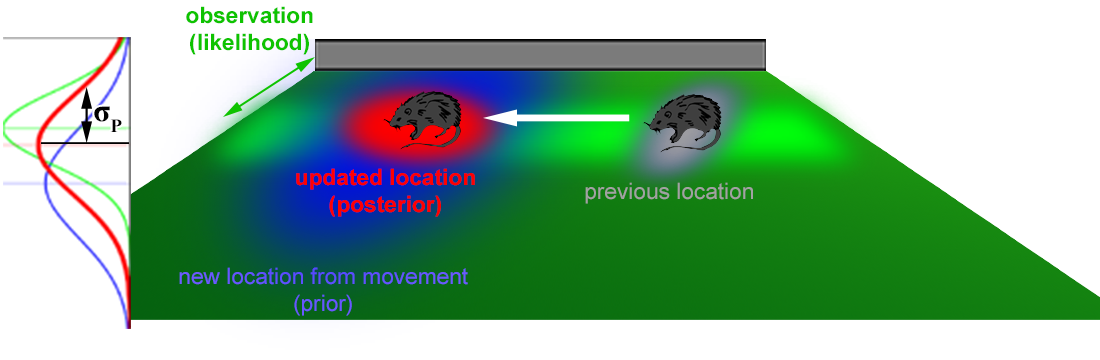
\includegraphics[width=\textwidth]{img/bayesian_localization3}
	\caption[Bayesian cue integration for localization]{\textbf{Bayesian cue integration for localization.} Illustration of how an animal might use its prior location belief (blue) estimated from its movement, and distance distributions e.g. to a boundary (green) to obtain a corrected location estimate (red) using Bayesian inference.} 
	\label{fig:bayescue} 
\end{figure}

%
\section{Bayesian localization}
\label{sec:bayesloc}

To maintain a location estimate through time, the kind of cue integration described above has to be performed regularly (after every time step). One source of location information is adding up each movement vector, a process called odometry in robotics and `path integration' in cognitive science and biology. However, movements are not accurate and noise free in real-world environments - each movement vector contains a slight error, and these errors add up over time. Eventually, these accumulating errors render the location estimate useless, if sensory information is not used to correct it. 

Bayesian localization is concerned with correcting the location estimate in time using noisy observations \citep{thrun2005probabilistic}. Conceptually, it entails performing the Bayesian cue integration to correct location estimates \textit{recursively}, after every movement / time step. Its operation can be summarized in three stages, which are performed iteratively at every time step: 1) movement (adding the current movement), 2) correction of the location estimate via Bayesian cue integration, 3) updating of the path integration estimate for use in the next iteration.

Unlike the simplified treatment above, which has considered only one snapshot in time, Bayesian localization considers the posterior at any time step $t$. This posterior distribution has to depend on all movements until now: $\bm m_{1:t}$, on all observations until now: $ O_{1:t}$, as well as the locations of known landmarks $\bm l_{1:N}$. Extended by these dependencies, the posterior location distribution from Equation \ref{bayes1} becomes

%specifying the probability distribution of the current position $ x_{t} $ given motor commands $u$, measurements $z$, and landmarks $l$. This expression can be expanded using Bayes' rule,

\begin{equation}
\label{bayesloc1}
p(\bm x_{t} | \bm m_{1:t}, O_{1:t}, \bm l_{1:N}) = \gamma p(O_{t} | \bm x_{t}, \bm l_{1:N}) p(\bm x_{t} | \bm m_{1:t}),
\end{equation}

\noindent through simple application of Bayes' theorem. We can use the sum rule (with the sum replaced by an integral for dealing with continuous distributions) to model the `path integration' (odometry) mechanism which provides the prior in Equation \ref{bayesloc1}:

\begin{equation}
\label{prior}
p(\bm x_{t} | \bm m_{1:t}) = \int p(\bm x_{t} | \bm x_{t-1}, \bm m_{t-1}) p(\bm x_{t-1} | \bm m_{1:t-1}) \mathrm{d} \bm x_{t-1}.
\end{equation}

This equation allows inferring the current location prior based on the most recent movement $\bm m_{t-1}$ and on the previous location estimate $\bm x_{t-1}$ by marginalizing (integrating out) the previous location. This is a recursive formulation which yields a path integration estimate based on a starting location and a number of movements. This estimate is subject to accumulating errors. However, crucially, the corrected previous location estimate (previous posterior) can be used instead of the uncorrected previous path integration estimate. Using this insight, replacing $p(\bm x_{t-1} | \bm m_{1:t-1})$ in Equation \ref{prior} by the previous location posterior $p(\bm x_{t-1} | \bm m_{1:t-1}, O_{1:t-1}, \bm l_{1:N})$ and plugging the resulting prior into Equation \ref{bayesloc1} yields

\begin{equation}
\label{bayeslocsolution}
\begin{split}
p(\bm x_{t} | \bm m_{1:t}, O_{1:t}, \bm l_{1:N}) = \gamma p(O_{t} | \bm x_{t}, \bm l_{1:N}) \int p(\bm x_{t} | \bm x_{t-1}, \bm m_{t-1}) \cdot \\
 p(\bm x_{t-1} | \bm m_{1:t-1}, O_{1:t-1}, \bm l_{1:N}) \mathrm{d} \bm x_{t-1}
\end{split}
\end{equation}

This recursive equation for updating location estimates is a Bayes-optimal solution to the localization problem and allows inferring the current location based on two conditional densities: a model specifying the effect of movements on the location (a `motion model'):
\begin{equation}\label{motionmodelq}
p(\bm x_{t} | \bm x_{t-1}, \bm m_{t-1})
\end{equation}
and a model specifying the probability distribution of the current measurements $ O_{t} $ at a position $ \bm x_{t} $ given the landmarks $ \bm l_{1:N} $ (a `sensor model'):
\begin{equation}\label{sensormodelq}
p(O_{t} | \bm x_{t}, \bm l_{1:N}).
\end{equation}

Equation \ref{bayeslocsolution} is the mathematical formulation of Bayesian localization, which, conceptually, iterates over the three stages mentioned above: movement (application of the motion model), correction (via Bayes' theorem), and update.

As argued in Chapter \ref{cha:bayespc} and Appendix \ref{apx:bayespc}, the activity of hippocampal place cells can be viewed as samples from probability distributions, and the size of their firing fields can be partially predicted by a Bayesian model. We will also argue based on existing evidence that the `motion model' is implemented by a neural path integrator in the entorhinal cortex, and that neurons with boundary-related firing might implement the `sensor model'.

Such a sampling-based representation of uncertainty in these spatially relevant brain areas naturally suggests employing a sequential Monte Carlo method \citep{doucet2000sequential} to computationally evaluate the integral in equation \ref{bayeslocsolution} (the same model using samples for representation might as well use them for inference). Although the usual method of choice in robotics is importance sampling \citep{montemerlo2007fastslam, thrun2005probabilistic}, we approximate the integral using rejection sampling \citep{doucet2000sequential}, and will argue in Chapter \ref{cha:bayespc} and Appendix \ref{apx:bayespc} that coincidence detection (CD) in hippocampal place cells can implement this mechanism (since CD can filter out samples at locations where different measurements and path integration disagree, and keeps the ones where they agree - see illustration in Figure \ref{fig:neurimpl}C, and Appendix \ref{apx:bayespc} for mathematical details). 

From a computational point of view, instead of inferring the parameters of the location posterior distribution (e.g. the mean and variance in case of a Gaussian), we represent it by sampling multiple location hypotheses. The mean of these hypotheses corresponds to the 'best guess' estimate, and their standard deviation to the associated uncertainty. Apart from the empirical evidence for sampling based mechanisms in the brain (see Chapter \ref{cha:bayespc}, as well as \citep{fiser2010statistically} for a more general review), the main advantage of this approach is the ability to represent free-form distributions (irregular, non-Gaussian, multimodal distributions etc.).

Particles (samples, hypotheses) $\bm x^i$ are generated regularly based on self-motion information (linear and angular movement speed $v$) according to the motion model (Equation \ref{motionmodelq}), performing path integration - in the simplest case: $ \bm x_{t}^i = \overline{\bm x}_{t-1} + \bm v'\Delta t $ - at simulated timesteps $ \Delta t $. Gaussian noise is multiplied to the estimated speed to obtain a distribution of hypotheses reflecting the path integration / odometry uncertainty (neither animals nor robots can estimate their movement speed with perfect accuracy):

$\bm v' = \bm v_{true} \cdot \mathcal{N}(\bm 1, \begin{bmatrix}\sigma_v^2 & 0\\ 0 & \sigma_\omega^2\end{bmatrix}) $,

\noindent where $ \sigma_v^2 $ and $ \sigma_\omega^2 $ are model parameters representing the variance in the linear and angular speeds, respectively. Since the estimate of $\bm v$ is noisy, accumulating errors would lead to an increase of uncertainty and the corruption of the distribution represented by the set of particles, which is why correction with the sensor model is required. 

Under Gaussian assumptions, this correction can be implemented simply by multiplying a path integration prior and a number of sensory likelihoods and solving for the means and variances (Equation \ref{bayes2}). The ensuing algorithm for Bayesian localization is trivial. When using samples instead of a Gaussian to represent the posterior, the correction can be implemented by rejection sampling \citep{doucet2000sequential}, i.e. by deleting hypotheses inconsistent with sensory measurements (see Figure \ref{fig:bayesloc}). The derivation of why this rejection sampling scheme approximates the true Bayesian posterior can be found in Appendix \ref{apx:bayespc}. Details regarding how brains could implement this algorithm are discussed in Chapter \ref{cha:bayespc}.

\begin{figure}[h]
	\begin{pseudocode}{movement}{samples, \textbf{v}, N}
		1: prevmean \GETS mean(samples) \\
		2: newsamples \GETS \{ \} \\
		3: \FOREACH particle \in samples \\
		4: \quad newsamples \GETS newsamples \cup {motionModel(particle, \textbf{v})} \\
		5: \WHILE count(newsamples) < N \\
		6: \quad newsamples \GETS newsamples \cup {motionModel(prevmean, \textbf{v})} \\
		7: return(newsamples)
	\end{pseudocode}
	\begin{pseudocode}{correction}{samples, \textbf{O}, \textbf{L}}
		1: newsamples \GETS \{ \} \\
		2: \FOREACH particle \in samples \\
		3: \quad likelihood \GETS sensorModel(particle, \textbf{O}, \textbf{L}) \\
		4: \quad \IF random() < likelihood \\
		5: \quad \quad newsamples \GETS newsamples \cup {particle} \\
		6: return(newsamples)
	\end{pseudocode}
	\begin{pseudocode}{localizationStep}{posteriorsamples, \textbf{v}, \textbf{O}, \textbf{L}, N}
		1: timestep++ \\
		2: movedsamples \GETS movement(posteriorsamples, \textbf{v}, N) \\
		3: correctedsamples \GETS  correction(movedsamples, \textbf{O}, \textbf{L}) \\
		4: return(correctedsamples)
	\end{pseudocode}
	\centering
	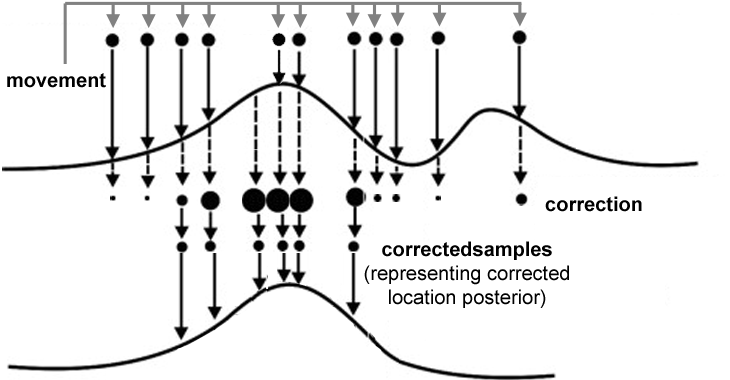
\includegraphics[width=0.75\textwidth]{img/rejectionsampling}
	\caption[Bayesian localization algorithm with rejection sampling]{\textbf{Bayesian localization algorithm with rejection sampling,} producing updated posterior samples given the samples from the previous posterior, speed vector $\bm v$ and observations $O$ at the current time step, landmarks $L$, and a particle budget $N$}
	\label{fig:bayesloc}
\end{figure}

%To correct this distribution, and to estimate the target posterior distribution \eqref{bayeslocsolution}, each particle is weighted according to the likelihood of the perceived sensory measurements from the location hypothesis represented by the particle, i.e. according to the sensor model: 
%$\bm w_t^i=p(O_t|\bm x_t^i, O_{t-1}, \bm m_t)$. This approach of estimating a target distribution is called importance sampling (see e.g. \cite{montemerlo2007fastslam, thrun2005probabilistic} for the derivation).

\section{Maximum likelihood map error correction}
\label{sec:bayescorr}

Landmark location estimates can be updated in the same way as the agents' location estimates $\bm x$, by integrating new observations into the posterior distribution representing these locations (either in the form of Gaussians or of samples from this distribution). With infinitely many particles, the algorithm presented in Figure \ref{fig:bayesloc} would suffice to maintain correct location estimates. 

However, there are practical limits on the particle budget (due to limited computational resources in computers, and due to limited firing rates in neurons). This neces-

\clearpage

\noindent sarily leads to errors whenever there is no particle at the unobservable true location. Unfortunately, these errors add up as well. They become most pronounced when revisiting an already known part of the environment, i.e. when traversing a loop - although the agent has returned to its starting location, it will think that it is at a new location, and form new representations of the same place. Multiple such loops can lead to multiple redundant, erroneous representations. 

The problem of how to correct spatial representations when revisiting a known place (not only the location estimate but also the estimated recent path and landmark locations) is the `loop closing' problem in robotics (see e.g. \citep{williams2009comparison, thrun2008simultaneous}). Brains need to solve this problem as well - although human spatial representations are not perfectly accurate, humans are able to correct mistaken estimates when they recognize a revisited place. Interestingly, despite the abundant robotics literature on the topic of closing loops, this problem has been largely neglected in cognitive science literature. 

Our cognitive model of loop closing is described in more detail Chapter \ref{cha:lida}. Here, we will briefly summarize its purely computational and mathematical aspects. We will assume that it is sufficient to correct the route taken during the loop, i.e. the most recent locations of the agent; and that the landmarks are corrected by the same amount as the location closest to them. That is, when performing large-scale loop closing, the model in Chapter \ref{cha:lida} applies the same correction to a position and the local landmarks around it (a simplification justified based on neuroscientific evidence in that Chapter). We also make the assumption that correction only concerns position representations and not angular representations, once again based on neural evidence. Hippocampal `reverse replay' \citep{carr2011hippocampal} (the re-activation of recently active place cells) is a plausible mechanism for correcting the recent route when revisiting a location, as argued in Chapter \ref{cha:lida}, but such a mechanism has not been found for neurons with direction-specific firing.

When revisiting a known place, the recently traversed path has to be corrected using the discrepancy between the previously and recently estimated location of the revisited place. Naturally, when an agent recognizes that it is in the same place it has visited before, the current estimate has to be reset to be equivalent to the previous estimate of the same location. However, it is not obvious how to correct the other recently visited locations $\bm x_0, ..., \bm x_m \in X$ along the recent path $X$. Let $\bm c_1, ... \bm c_m \in C$ denote a set of vectors we will call constraints, each expressing how far apart two locations should be according to some measurement. That is, each constraint specifies the difference between two locations $\bm c=\bm x_a-\bm x_b$, and each is associated with a measurement uncertainty $S_c$ in the form of the covariance matrix of a normal distribution. For locations traversed in sequence, $\bm c$ and $S_c$ is given by the motion model (by path integration). For revisited locations, $\bm c$ is zero. 

According to Bayes' theorem, and assuming that constraints are independent given the location, the recent path depends on the product of the constraint distributions; and the best path estimate is the one that maximizes:

\begin{equation}
\label{loopprob}
P(X|C) \propto \prod_{i=1}^{m} P(\bm c_i|X) 
\end{equation}

Each $P(\bm c_i|X)$ expresses the likelihood that this constraint is satisfied by the path $X$, as a Gaussian distribution: $P(\bm c_i|X)\propto\mathcal{N}(\bm x_a-\bm x_b;\bm c_i, S_i)$ (where $\bm x_a$ and $\bm x_b$ are the location estimates which should have the distance $\bm c_i$ according to this constraints). We are interested in the maximum of Equation \ref{loopprob}, which is equivalent to the minimum of its negative logarithm. Let $\bm d_i=\bm x_a - \bm x_b - \bm c_i$ be the discrepancy between the constraint and the locations it concerns within the path. With noise-free measurements, all $d_i$ would be zero; but since sensory errors may add up, there will be discrepancies (e.g. after traversing a loop, the estimate of the first visit $\bm x_a$ and second visit $\bm x_b$ may differ, but $\bm c_i=0$ for the revisited place). Then, the most likely path is given by:

\begin{equation}
\label{mleq}
X_{ml} = \argmax_X P(X|C) = \argmin_X -log P(X|C) = \argmin_X \sum_{i=1}^{m} ||\bm d_i||_{S_i^{-1}}.
\end{equation}

Equation \ref{mleq} mathematically describes the maximum likelihood error correction problem for loop closing. It tries to minimize the discrepancies between the constraints and the estimated locations, taking into account the constraint uncertainties $S_i$ by utilizing the Mahalanobis distance\footnote{The Mahalanobis distance is defined as $||\bm x_1-\bm x_2||_S = \sqrt{(\bm x_1-\bm x_2)^TS(\bm x_1-\bm x_2)}$} to measure the discrepancy.

There are several ways to solve Equation \ref{mleq}. For our cognitive model (Chapter \ref{cha:lida}), we chose sequential gradient descent, because it can be implemented in biological neurons \citep{bengio2015towards}. \cite{olson2006fast} derive the starting point for this solution. They suggest the following gradient with respect to constraint $i$, depending on a learning rate $\alpha$, a full Jacobian $J$ of the constraints with respect to the path, and the Jacobian $J_i$ of constraint $i$:

\begin{equation}
\label{gradient}
\Delta X \approx \alpha (JS^{-1}J)^{-1}J_i^TS_i^{-1} \bm d_i.
\end{equation}

Because of the incremental structure of the Jacobian, it is possible to simplify this expression (see Chapter \ref{cha:lida}). Making use of this structure, and defining a loop precision parameter $A_i=S_i/S_P$ specifying the ratio of the uncertainties of loop closure constraints (added when revisiting a place) and path integration constraints, the gradient for each individual location within the loop becomes:

\begin{equation}
\label{correction}
\Delta \bm x_j \approx \alpha d_i \frac{\sum_{k=a+1}^{j} S_i^{-1}}{\sum_{k=a+1}^{min(j,b)} S_P^{-1}} = \alpha A_i \bm d_i p_j,
\end{equation}

\noindent where $p_j=(min(j,b_i)-a_i-1)/(b_i-a_i-1)$ denotes how far $x_j$ lies along the loop, with $0 \leq p_j \leq 1$. Unlike usual gradient descent procedures, in this particular case we know that $\Delta \bm x \leq \bm d_i $ must hold, and can prevent the algorithm from overshooting, accelerating its convergence. Figure \ref{fig:sgdslam} contains the algorithm using this gradient to correct location estimates when revisiting a place. We will use this algorithm in Chapter \ref{cha:lida} to account for human cognitive map accuracy, as a part of a cognitive architecture embodied on a robot and learning maps in realistic simulated environments.

\begin{figure}[h]
	\begin{pseudocode}{correctPath}{X, loopConstraints, \alpha, A, N}
		1: \WHILE i < N \AND \NOT converged \\
		2: \quad i++ \\
		3: \quad \FOREACH a,b \in loopConstraints \\
		4: \quad \quad discrepancy \GETS X_a - X_b \\
		5: \quad \quad \FOREACH j \in (a,b] \\
		6: \quad \quad \quad p \GETS (min(j,b)-a-1)/(b-a-1) \\
		7: \quad \quad \quad \beta \GETS min(\alpha A \cdot discrepancy, discrepancy) \\
		8:\quad\quad\quad X_j \GETS X_j + \beta p \\
		9: return(X)
	\end{pseudocode}
	\caption[Algorithm for correcting location estimates when revisiting places]{\textbf{Algorithm for correcting location estimates when revisiting places (`loop closing'),} producing a corrected path given the estimates of locations $X$ along that path (from Bayesian localization), a list of loop constraints indicating the same (revisited) places (from landmark recognition or place recognition), a learning rate $\alpha$, a loop precision parameter $A$ and an iteration budget $N$}
	\label{fig:sgdslam}
\end{figure}

\section{Bayesian nonparametrics for map structuring}
\label{sec:bayesmap}

It has been suggested that map-like spatial representations are structured hierarchically \citep{hirtle1985evidence,mcnamara1989subjective,greenauer2010micro}, but no formal model has been put forth for a process that might account for this structure. We hypothesize in Chapter \ref{cha:structure} that this process might be clustering. Computationally, we chose a Dirichlet Process Gaussian Mixture Model (DP-GMM) to account for the behaviour data we collected (see Chapter \ref{cha:structure}), for two reasons. First, DP-GMMs (unlike most clustering algorithms) are able to infer the number of clusters, not just cluster memberships; and are infinitely extensible \citep{rasmussen1999infinite}. Second, Bayesian nonparametric models with Dirichlet priors have a successful history in psychological modelling, e.g. of category learning and causal learning \citep{tenenbaum2011grow}, transfer learning \citep{canini2010modeling}, and human semi-supervised learning \citep{gibson2013human}.

By `map structure', here and in Chapter \ref{cha:structure}, we mean sub-map memberships. There is evidence that human spatial maps are hierarchical \citep{hirtle1985evidence,mcnamara1989subjective,greenauer2010micro}, just as geographical maps are - e.g. there is a map of the country and a map of the cities therein; and any given building may be represented not only on the country map but also on one of the city maps. Similarly, any object (e.g. building) memorized by a participant belongs to her map-like spatial representation (`cognitive map'), as well as to one of its sub-maps. We only consider a two-level hierarchy (map and sub-maps); thus, sub-map memberships fully describe our modelled map structure.

A number of features can influence spatial representation structure, including spatial distance and visual and functional similarity of landmarks. The importance of these features varies across participants, and these subject-specific importances have to be accounted for before the clustering process. We chose to implement a new metric learning method to do so (see below). Our model of spatial representation structure consists of these two components: a subject-specific metric, expressing the `similarity function' between two buildings, and the DP-GMM model for clustering buildings under this metric.

As noted in the Introduction, unlike the rest of our work, we have not shown what the neural implementation of such a structuring process might look like. Some prior work exists showing the possibility of inference in hierarchical Bayesian models such as the DP-GMM, e.g. \citep{shi2009neural} - see \citep{sanborn2015types} for a review. We have substantiated the psychological plausibility of this model by showing that it can explain and predict human behavior data (Chapter \ref{cha:structure}), and leave the investigation of the biological plausibility of this specific mechanism for future work.

\subsection{Dirichlet Process Gaussian Mixture Models for clustering}

We will only describe the DP-GMM model very briefly, since it is a well-established model and since we did not implement it ourselves in this work (we used the $bnpy$ Python library instead). See e.g. \citep{rasmussen1999infinite} for its introduction, or \citep{gershman2012tutorial} for a tutorial. The DP-GMM partitions a number of data points $x$ into $K$ clusters by fitting a mixture of $K$ Gaussian distributions to the data. It infers the number of clusters, as well as the means $\bm \mu_k$ and covariances $\Sigma_k$ of each Gaussian, by inverting the generative process defined as follows:
 
\begin{equation}
\label{eq:dpgmm}
\begin{array}{rcl}
\phi_k   \sim Beta(1, \alpha_1) \\
\bm \mu_k    \sim Normal(0,  \mathbf{I}) \\
\Sigma_k \sim Wishart(D, \mathbf{I}) \\
\pi_{k}  \sim SBP(\phi) \\
\bm x_t \sim Normal(\bm \mu_{z_i},  \Sigma_{z,i}^{-1}),
\end{array}
\end{equation}

\noindent where SBP stands for the stick-breaking process for generating mixture weights: $\pi_k=v_k \prod_{j=1}^{k-1} (1-v_j)$. Data can be generated from this model by first choosing a cluster with probabilities specified by mixture weights: $z \sim Cat(\pi)$, and then drawing an observation from the parameters of that cluster $\bm x \sim Normal(\bm \mu_z, \Sigma_z)$.

Given the data, the parameters of this model can be inferred using either a Monte Carlo chain sampling method \citep{neal2000markov} or variational inference \citep{blei2006variational}. We did not implement an inference algorithm in this work; instead, we have used the $bnpy$ Python library for this purpose. See \citep{hughes2013memoized} for implementation details.

\subsection{Metric learning in absolute pairwise difference space}

In order to learn a suitable metric for our data, we had to develop a novel metric learning method, since the assumptions made by existing methods do not hold in our case. Neither the linear separability assumption (made by linear metric learning), nor the prerequisite of roughly isotropic variances along the features (made by RBF-based methods \citep{ong2005learning}) is the case for all subjects in our dataset (see Appendix E for further motivation and evaluation from a machine learning perspective). 

Furthermore, our metric can naturally incorporate the hypothesis that building pairs belonging to the same representation should be located close to the origin in pairwise difference space (i.e. they should not be very different), and should be separable from building pairs belonging to different representations. These two distributions of pair differences can be naturally modelled using Gaussian distributions - see Chapter \ref{cha:structure}. 

Our proposed method can be seen as a novel approach to perform non-linear metric learning using weak supervision in the form of pairwise constraints, in order to improve clustering performance, as pioneered by \cite{xing2002distance}. The problem to be solved can be defined as follows. Let $\mathcal{X}=(\bm x_i, ..., \bm x_n)$ be the feature vector representation of $n$ objects (buildings on a cognitive map) which are to be clustered (assigned to representations we will call `sub-maps'), where $\bm x_i \in \mathbb{R}^D$ are vectors with $D$ dimensions. Let the set of $m$ given labelled pairwise co-representation constraints be denoted by $\mathcal{C}$, where $ \lvert \mathcal{C} \lvert = m $, and $c_{i,j} \in \mathcal{C}$ is

\begin{equation}
c_{i,j}=
\begin{cases}
1, & \text{if $i$ and $j$ belong to the same sub-map (co-represented)} \\
0, & \text{if $i$ and $j$ belong to different sub-maps (not co-represented)}
\end{cases}
\end{equation}

Our ultimate goal is to group the $n$ objects into $K$ clusters (`sub-maps'), such that objects of the same cluster are more similar to each other than to those of different clusters; taking into account the provided pairwise constraints to learn a good similarity metric for the given data.

Conventional approaches leveraging non-linear metric learning for this problem try to find a kernel $\Phi$ such that the clustering resulting from using the distance metric defined by that kernel, $d_m^2(\bm x_1, \bm x_2)=(\Phi(\bm x_1)-\Phi(\bm x_2))^T(\Phi(\bm x_1)-\Phi(\bm x_2))$, does not violate the provided constraints (ensures co-represented pairs are closer than other pairs, if possible), and often employ RBF kernels for this purpose, e.g. \citep{baghshah2010kernel, chitta2011approximate}. 

In contrast, the proposed framework aims to learn the distribution of co-representation probabilities (whether or not two object should be linked) from the provided set of constraints, and constructs a pseudo-metric based on a generative model of co-representation probabilities. Crucially, this probabilistic model is defined on the vector space of absolute pairwise differences (APD), which allows learning the importance of each feature (a challenge for RBF kernels for data with non-isotropic variance). Learning in APD space has been proposed before by \cite{zheng2011person} (specifically for person re-identification in computer vision), but not as a general metric learning method. The metric based on this generative model is a pseudo-metric, because it does not satisfy the conditions of subadditivity, $d_m(\bm x, \bm z) \leq d_m(\bm x, \bm y)+d_m(\bm y,\bm z)$ and the identity of discernibles, $d_m(\bm x, \bm y) = 0 \enskip \text{if and only if} \enskip \bm x = \bm y$.

Let $[\Delta \bm{x_{i,j}}]_+ = \big( \lvert \bm{x_{i,k}} - \bm{x_{j,k}} \lvert \big)_{k=1}^m $ be the representation of each pair of objects $(i,j)$ in APD vector space. The co-representation probability distribution, i.e. the posterior probability of any pair of objects belonging to the same cluster, given a pair of objects and some model parameters $\bm{\theta}$ is then 

\begin{equation}
\label{eq:linkprob}
p(c=1|\Delta \bm{x}, \bm{\theta}) \propto p(\Delta \bm{x} | c=1, \bm{\theta}) p(c=1|\bm{\theta})
\end{equation}

The likelihood $ p(c=1|\Delta \bm{x}, \bm{\theta}) $, the model parameters $ \bm{\theta} $ (as well as the prior) can be estimated from $\mathcal{X}$ and $\mathcal{C}$, even in closed form, using Gaussian Discriminant Analysis (GDA). This yields a suitable non-linear pseudo-metric based on this probability distribution - see Equation \ref{eq:metric} -, such that objects likely to belong to the same cluster will be close, and those likely to belong to different clusters will be far apart; with these distances directly depending on co-representation probabilities. 

\begin{equation}
\label{eq:metric}
d_m(\bm x_1, \bm x_2; \bm{\theta}) = 1 - p(c=1|\Delta \bm x, \bm{\theta}) = p(c=0|\Delta \bm x, \bm{\theta})
\end{equation}

A metric is well-suited for clustering if within-cluster instances are closer than across-cluster instances according to it. That is, if for any co-represented $\Delta \bm x_r$ and not co-represented $\Delta \bm x_n $ it holds that $ d_r(\bm x_{r,1}, \bm x_{r,2}; \bm{\theta}) < d_n(\bm x_{n,1}, \bm x_{n,2}; \bm{\theta}) $. It follows from Equation \ref{eq:metric} that this is the case if the generative model learns to separate the absolute differences of within-cluster instance pairs from across-cluster pairs.

In the generative \textbf{GDA} model \citep{bensmail1996regularized}, the likelihoods of a pair of instances either being co-represented (i.e. belonging to the same sub-map), or not being co-represented (i.e. belonging to different sub-maps) are each modelled using a multivariate Gaussian: 

\begin{equation}
\label{eq:mvnormal}
p( \Delta \bm x | c=i; \bm \mu_i, \Sigma_i) = (2\pi)^{-\frac{D}{2}}|\Sigma_i|^{-\frac{1}{2}}\, e^{ -\frac{1}{2}(\Delta \mathbf{x}-\bm\mu_i)^\intercal\Sigma_i^{-1}(\Delta \mathbf{x}-\bm\mu_i) },
\end{equation}

\noindent where $i \in \{0,1\}$. $(\bm \mu_1, \Sigma_1)$ are the means and covariances of the APD distances of co-represented pairs, and $(\bm \mu_0, \Sigma_0)$ those of not co-represented pairs. These parameters can be easily estimated from the two given sets of co-represented and not co-represented object pairs, respectively, by calculating their means and covariances. 

From Equation \ref{eq:mvnormal} and Bayes' theorem, we obtain the generative probability required for the metric in \ref{eq:metric}, which then becomes:

\begin{equation}
\label{eq:adsgda}
d_m(\bm x_1, \bm x_2; \bm{\theta}) = 1 - \frac{p( \Delta \bm x | c=1; \bm \mu_1, \Sigma_1)}{\sum_{i \in \{0,1\}} {p( \Delta \bm x | c=i; \bm \mu_i, \Sigma_i)}}
\end{equation}

% The crucial difference between Equation \ref{eq:adsgda} and a simple RBF kernel is that the latter can be seen as a symmetric Gaussian `ball' in D-dimensional space, completely described by a single variance parameter. In contrast, the GDA-based model allows implicitly learning the importance of each feature, as well as their covariance, in a non-linear fashion (i.e. it can separate two sets of objects even if they are not linearly separable).

Thus, the trained GDA-model can be used to calculate distances (Equation \ref{eq:adsgda}) between all pairs of objects in any testing data set. The data is projected under the metric in Equation \ref{eq:adsgda} using distance-preserving embedding. We have used multi-dimensional scaling (MDS) for this purpose \citep{borg2005modern}. The result of this projection is a data set embedded such that Euclidean pairwise distances therein reflect the distances \ref{eq:metric} in the original dataset.

We subsequently perform clustering of this resulting data, using a Dirichlet Process Gaussian Mixture Model (DP-GMM) \citep{rasmussen1999infinite}, since the number of clusters is unknown (see previous section). The resulting algorithm for structuring map representations is shown in Figure \ref{fig:structalg}. It requires training data in the form of buildings for which it is known which representation they belong to (this can be inferred from recall lists of participants). We use this algorithm to predict the representation structure of participants' cognitive maps in advance in Chapter \ref{cha:structure}.

\begin{figure}[h]
	\begin{pseudocode}{predictMapStructure}{X, knownX, knownStructure}
		1: corepresented \GETS \{\} \\
		2: notcorepresented \GETS \{\} \\
		3: \FOR i \in (1, |knownX|) \\
		4: \quad \FOR j \in (i+1, |knownX|) \\
		5: \quad \quad \IF knownStructure_i = knownStructure_j \\
		6: \quad \quad \quad corepresented \GETS corepresented \cup (knownX_i-knownX_j) \\
		7: \quad \quad \textbf{else} \\
		8: \quad \quad \quad notcorepresented \GETS notcorepresented \cup (knownX_i-knownX_j) \\
		9: \ \ \mu_{co} \GETS mean(corepresented) \\
		10: \Sigma_{co} \GETS cov(corepresented) \\
		11: coprior \GETS \frac{|corepresented|}{|knownX|} \\
		11: \mu_{not} \GETS mean(notcorepresented) \\
		12: \Sigma_{not} \GETS cov(notcorepresented) \\
		13: notprior \GETS \frac{|notcorepresented|}{|knownX|} \\
		14: D \in \mathbb{R}^{|X|x|X|} \\
		15: \FOR i \in (1, |X|) \\
		16: \quad \FOR j \in (i+1, |X|) \\
		17: \quad \quad D_{i,j} \GETS 1 - \frac{coprior \cdot \mathcal{N}((X_i-X_j); \mu_{co}, \Sigma_{co})}{coprior \cdot \mathcal{N}((X_i-X_j); \mu_{co}, \Sigma_{co}) + notprior \cdot \mathcal{N}((X_i-X_j); \mu_{not}, \Sigma_{not})} \\
		18: embedding \GETS MDS(D) \\
		19: structure \GETS DPGMM(embedding) \\
		20: return(structure)
	\end{pseudocode}
	\caption[Algorithm for predicting spatial representation structure]{\textbf{Algorithm for predicting participants' spatial representation structure}, given the features of the new buildings to be structured, and given buildings with known structure (from a previous experiment) specifying which of these buildings were co-represented.}
	\label{fig:structalg}
\end{figure}

We point out that Equation \ref{eq:metric} constitutes a general framework for metric learning using any model capable of producing probability estimates that two instances belong together. This includes the entire family of generative models in machine learning (see e.g. \citep{bishop2006pattern}), as well as any discriminative model when combined with Platt scaling \citep{platt1999probabilistic} for transforming discrete outputs into probabilities. Two example applications of this general metric learning framework are semi-supervised clustering (extending the algorithm in Figure \ref{fig:structalg} by using semi-supervised GDA), or semi-supervised classification. See Appendix \ref{apx:adsmetric} for these examples and the evaluation of their performance with different constituent models.



%\section{Image processing, segmentation, and recognition}

%point out comp aspects WHEREVER POSSIBLE / APPROPRIATE 

%review of methods point out COMP./MATH

%point out what you can get / what you cant get, specifically saying limitations

%limitations 

%\section{Empirical methods}
%
%\subsection{Bayesian localization}
%
%The computational models presented below are based on the hypotheses summarized in Table \ref{tbl:hyp} in the Introduction. Previously gathered and published data was available for testing the hypotheses that hippocampal place cells might encode uncertainty and use it for approximate Bayesian inference, in the form of neural activity recorded using head-mounted intracranial electrodes in behaving rats in multiple environments, collected outside this PhD by \citep{burke2011influence, okeefe1996geometric, Odobescu2010} - see Chapter \ref{cha:bayespc}. Place cells also play a crucial role in human spatial memory \citep{ekstrom2003cellular}. But since the cognitive models below are concerned with human cognition, we additionally used human behaviour data published by \citep{nardini2008development} to evaluate the Bayesian localization model on a behavioural level. In this  see Chapter \ref{cha:lida}.
%
%\subsection{Bayesian nonparametric clustering}
%
%Although 
%
%\section{Computational methods} 

\chapter{Review of computational cognitive models of spatial memory}
\label{cha:nnreview}

\textbf{Publication 1 / 4.} Madl T., Chen K., Montaldi D. \& Trappl R., 2015. Computational cognitive models of spatial memory in navigation space: A review. \textit{Neural Networks, 65, 18-43.}

\newpage

\addtocounter{page}{-1}

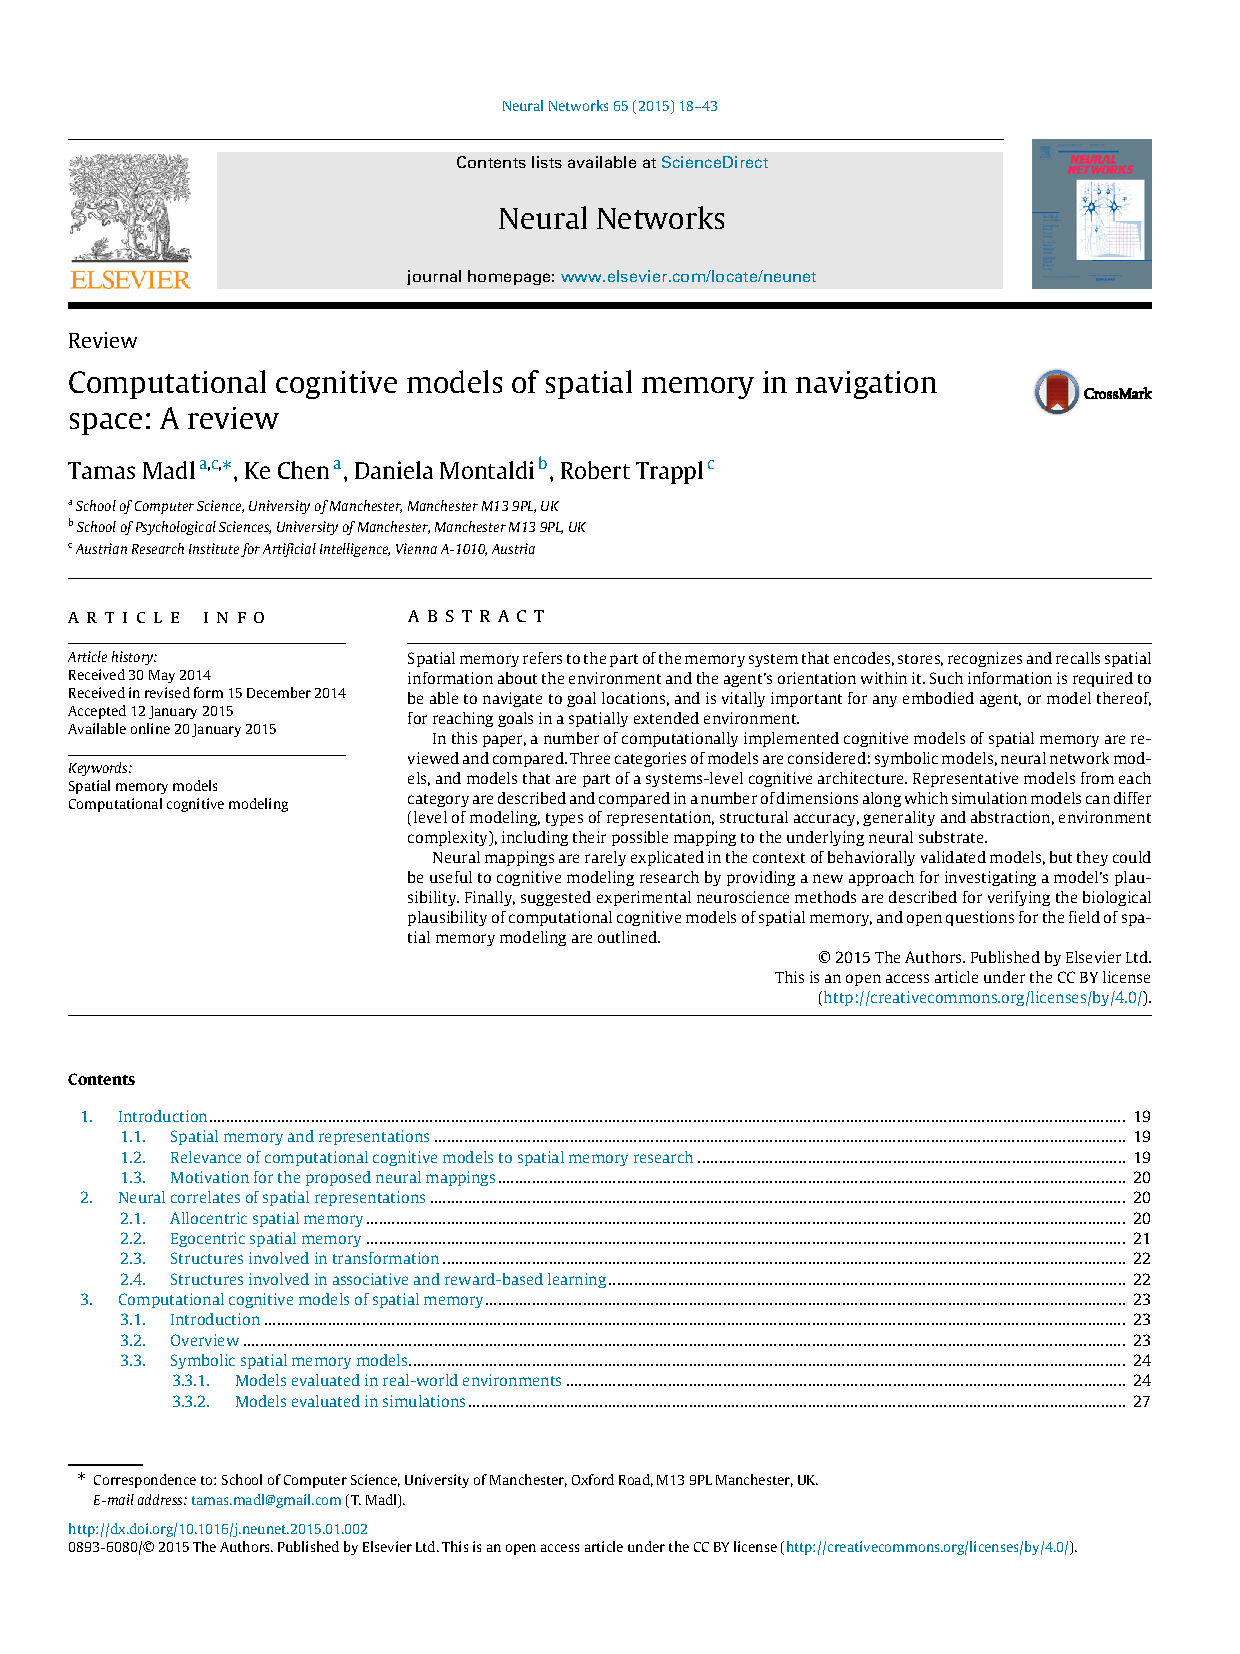
\includepdf[pages={-}, 
addtolist={
	1, figure, {Grid cells, place cells, boundary-related cells, head-direction cells, and the neuronal basis of self-motion information (p. 21)}, fig:nnrev:gcpcbvc,
	1, figure, {Overview of symbolic models evaluated in real-world environments (p. 25)}, fig:nnrev:symrl,
	1, figure, {Overview of symbolic models evaluated in simulated environments (p. 28)}, fig:nnrev:symsim,
	1, figure, {Two navigation strategies (p. 29)}, fig:nnrev:navstrat,
	1, figure, {Overview of neural network models evaluated in real-world environments (p. 30)}, fig:nnrev:nnrl,
	1, figure, {Overview of neural network models evaluated in simulated environments 1 (p. 32)}, fig:nnrev:nnsim1,
	1, figure, {Overview of neural network models evaluated in simulated environments 2 (p. 32)}, fig:nnrev:nnsim2,
	1, figure, {Overview of cognitive architectures evaluated in simulations 1 (p. 35)}, fig:nnrev:cogarch1,
	1, figure, {Overview of cognitive architectures evaluated in simulations 2 (p. 35)}, fig:nnrev:cogarch2,
	1, table, {Characteristics of the reviewed models (pp. 38-39)}, tbl:nnrev:char
}]{papers/nnreview.pdf}

\addtocounter{page}{-25}

\chapter{Bayesian integration of information in hippocampal place cells}
\label{cha:bayespc}

\textbf{Publication 2 / 4.} Madl T., Franklin S., Chen K., Montaldi D. \& Trappl R., 2014. Bayesian Integration of Information in Hippocampal Place Cells. \textit{PLoS ONE 9(3), e89762}

\vspace{1cm}
 
\textit Note: the manuscript was originally published with incorrect figure ordering. The correct figure order was published as a correction (doi: 10.1371/journal.pone. 0136128), but PLOS has decided to maintain the old manuscript with incorrect ordering online. The reprint below contains the corrected figure order. No other changes have been made to the online version.

\newpage

\addtocounter{page}{-1}

\includepdf[pages={-}, 
addtolist={
	1, figure, {Place field sizes, and predicted uncertainty, on an empty rectangular track (p. 4)}, fig:bayespc:pfrect,
	1, figure, {Place field sizes, and predicted uncertainty, on a circular track with objects (p. 5)}, fig:bayespc:pfcirc,
	1, figure, {Predicted and recorded place fields in environment B (p. 6)}, fig:bayespc:pfb,
	1, figure, {Neuronal implementation of Bayesian inference based on coincidence detection (p. 8)}, fig:bayespc:cd,
	1, figure, {Density of place cell spikes, and predicted uncertainty, on a circular track with objects (p. 9)}, fig:bayespc:density,
	1, figure, {Place field sizes, and predicted uncertainty, on a circular track with objects, using the extended model (p. 10)}, fig:bayespc:pfextended,
	1, figure, {Errors of coincidence-based multiplication based on a simple integrate-and-fire model (p. 11)}, fig:nnrev:cderr
}]{papers/bayespc.pdf}

\addtocounter{page}{-15}

\chapter{The structure of spatial representations}
\label{cha:structure}

\textbf{Publication 3 / 4.} Madl T., Franklin S., Chen K., Trappl R. \& Montaldi D., submitted. Exploring the structure of spatial representations. \textit{Cognitive Processing}

\newpage

\addtocounter{page}{-1}

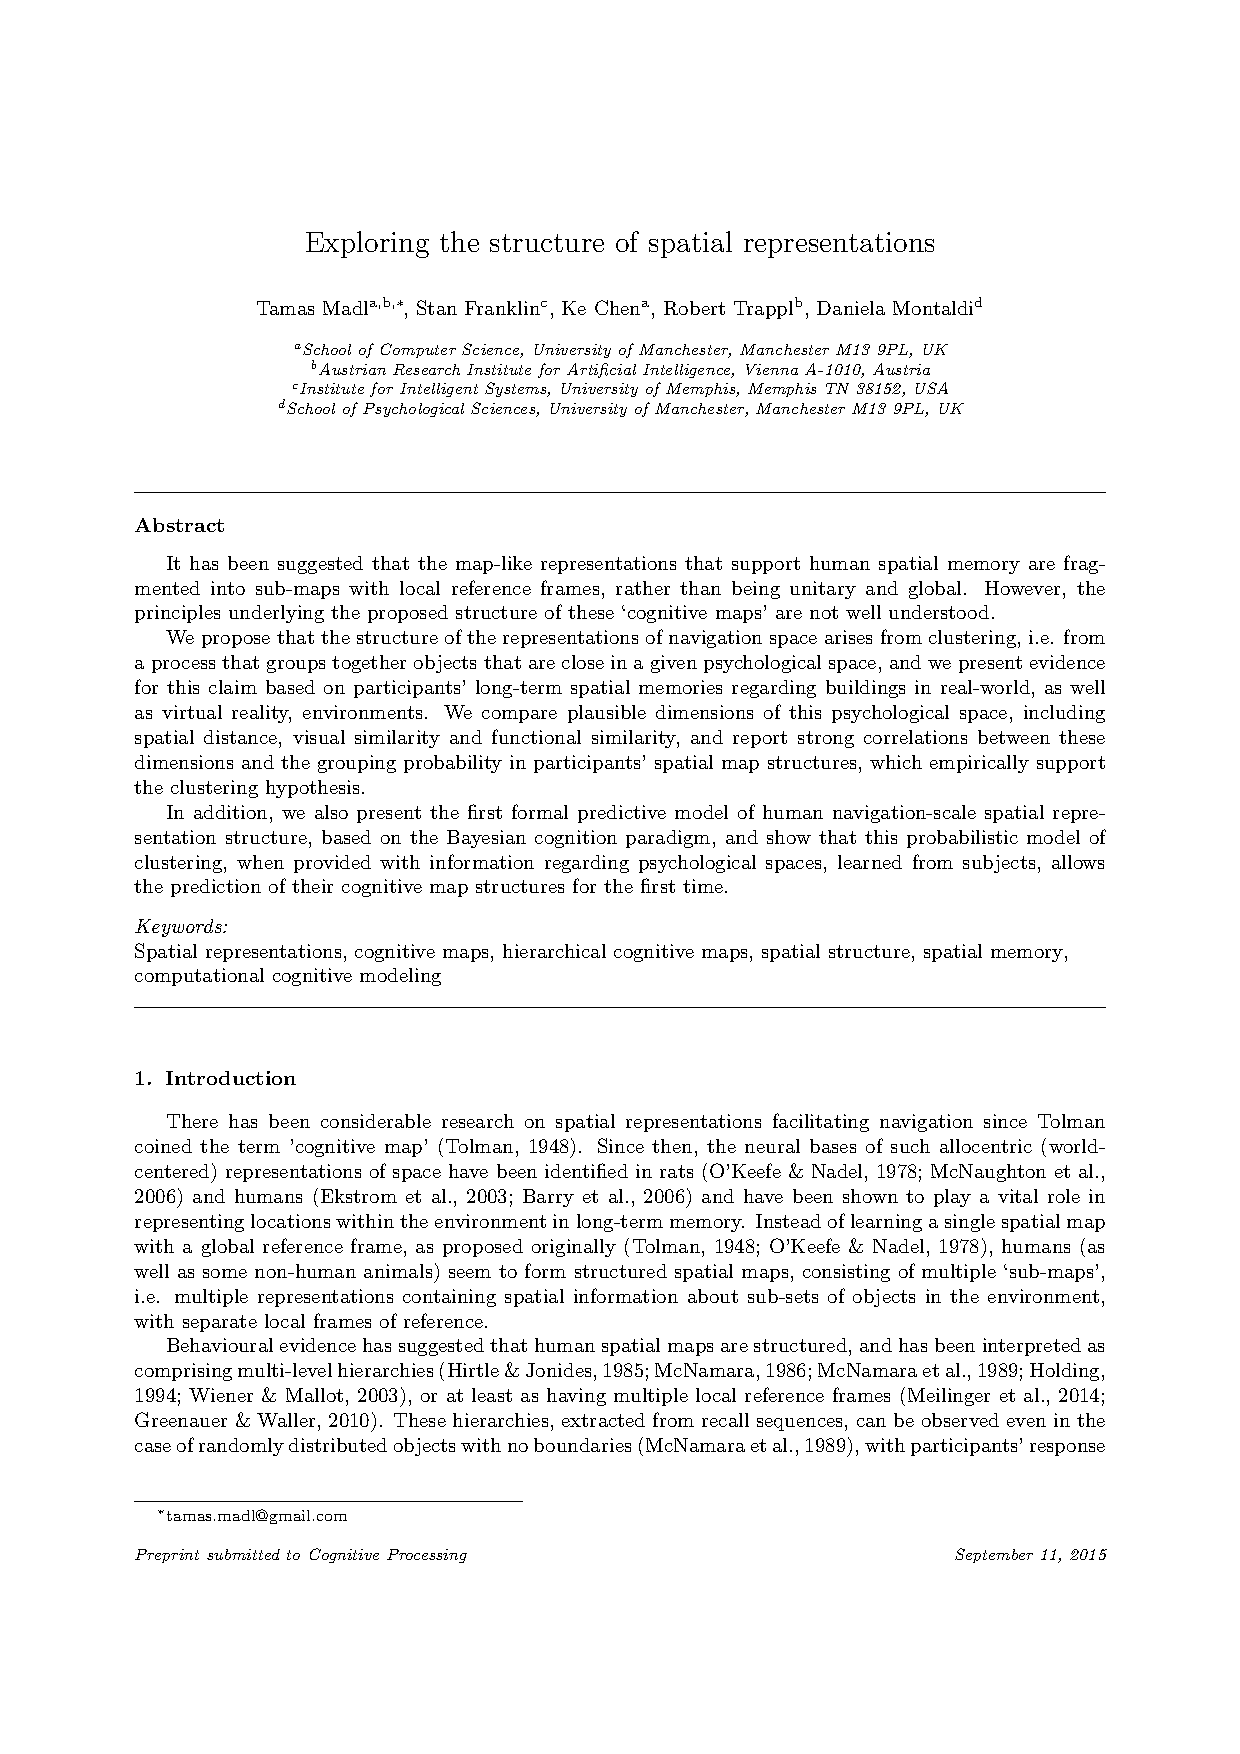
\includepdf[pages={-}, 
addtolist={
	1, figure, {Formalizing relative feature importances for grouping objects (p. 4)}, fig:mapstructure:formalizing,
	1, figure, {A part of the real-world memories experiment interface of Experiments 1 and 3 (p. 5)}, fig:mapstructure:rlscrn,
	1, figure, {A part of the virtual reality experiment interface of Experiment 2 (p. 6)}, fig:mapstructure:vrscrn,
	1, figure, {The recall sequence-based method used to extract cognitive map structure (p. 8)}, fig:mapstructure:recallsequence,
	1, figure, {Overview over the 149 cities in which participants' memory structures were inferred (p. 9)}, fig:mapstructure:map149,
	1, figure, {Correlations between probabilities of being on the same sub-map, and distances along each feature, (p. 16)}, fig:mapstructure:corr1,
	1, figure, {Variability of features influencing cognitive map structure (p. 17)}, fig:mapstructure:variability,
	1, figure, {The decision hyperplane method for inferring feature importances and generating environments (p. 19)}, fig:mapstructure:dechyp,
	1, figure, {Results of a predictive clustering model using subjects' feature importances, learned using the decision hyperplane approach (p. 22)}, fig:mapstructure:dechypresults,
	1, figure, {Learning subject-specific models for predicting cognitive map structure (p. 24)}, fig:mapstructure:gdaopt,
	1, figure, {Estimated maximum possible prediction rate using the data in Experiment 3 (p. 26)}, fig:mapstructure:maxpred,
	1, figure, {Accuracies obtained by predicting participant’s map structures using DP-GMM clustering under the learned subject-specific models (p. 29)}, fig:mapstructure:accuracies,
	1, figure, {Possible obstacles to predicting subject cognitive map structures (p. 33)}, fig:mapstructure:obstacles,
	1, table, {Effects of spatial representation structure on distance estimation, walking time estimation, and response times (p. 13)}, tbl:mapstructure:effects,
	1, table, {Prediction accuracies (and Rand indices) in Experiment 3 (p. 28)}, tbl:mapstructure:predacc
}]{papers/mapstructure.pdf}

\addtocounter{page}{-36}

\chapter{Towards real-world capable spatial memory in the LIDA cognitive architecture}
\label{cha:lida}

\textbf{Publication 4 / 4.} Madl T, Franklin S, Chen K, Montaldi D \& Trappl R, submitted. Towards real-world capable spatial memory in the LIDA cognitive architecture. \textit{Biologically Inspired Cognitive Architectures}

\newpage

\addtocounter{page}{-1}

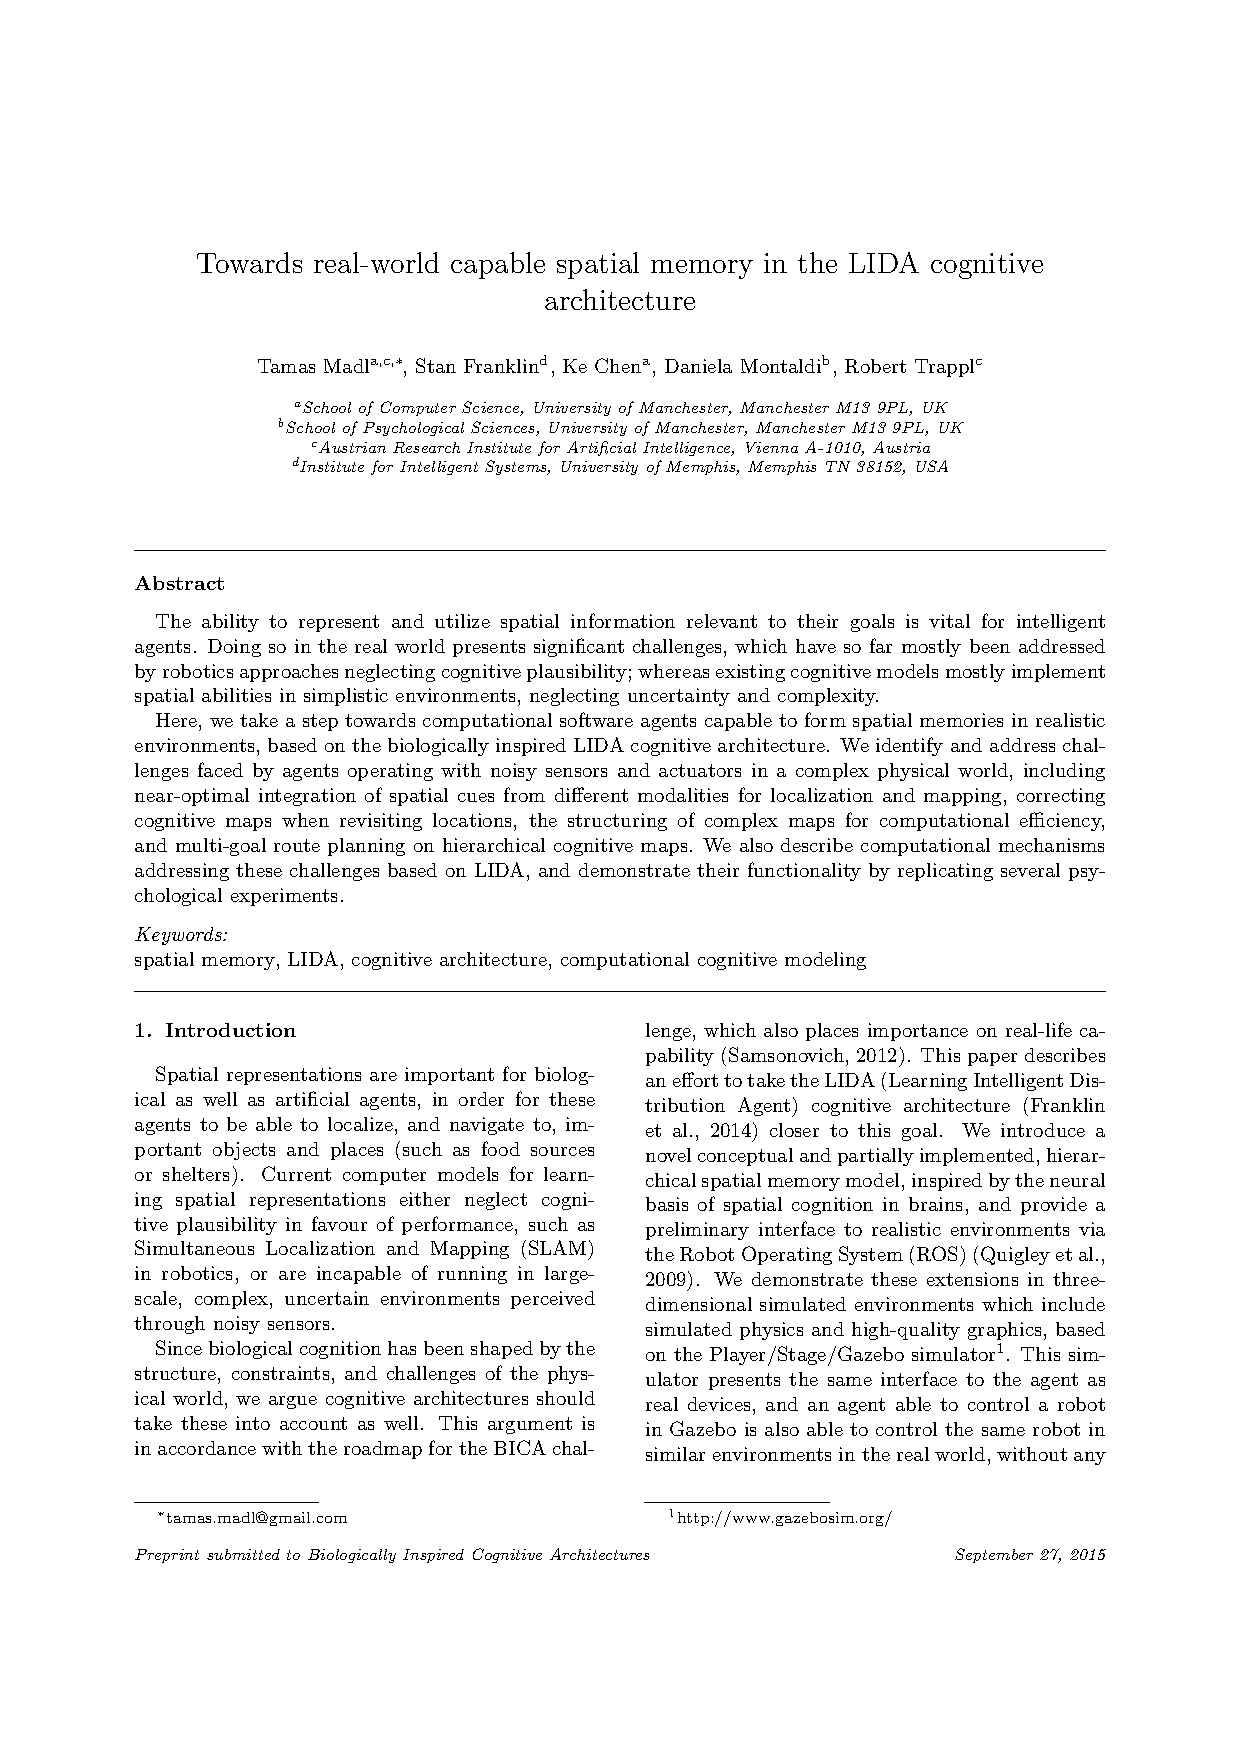
\includepdf[pages={-}, 
addtolist={
	1, figure, {Spatially relevant brain areas and LIDA modules (p. 5)}, fig:lida:brain,
	1, figure, {Extensions to add spatial abilities to LIDA (p. 7)}, fig:lida:extensions,
	1, figure, {Representations in Extended PAM in a simulated environment (p. 8)}, fig:lida:epam,
	1, figure, {Approximate Bayesian cue integration in spiking neurons (p. 10)}, fig:lida:apprbayes,
	1, figure, {Route planning on recurrently interconnected place nodes (p. 10)}, fig:lida:routeplanning,
	1, figure, {Loop closing performed by the Map correction SBC (p. 12)}, fig:lida:loop,
	1, figure, {Position errors and standard deviations in the cue integration experiment by Nardini et al. (2008) (p. 14)}, fig:lida:nardini,
	1, figure, {Comparison with human and model errors over all environments (p. 15)}, fig:lida:comparison
}]{papers/lidaspm.pdf}

\addtocounter{page}{-17}

\chapter{Discussion}
\label{cha:discussion}

\chapter{Conclusion}
\label{cha:conclusion}

Humans live and act in a world they can only partially observe through imperfect sensors and process with an inherently noisy information processing system. In mathematics, probability theory has provided a framework for the representation and manipulation of uncertainty \citep{jaynes1996probability}. In this thesis, we have argued for the necessity of such a framework within the field of computational cognitive modelling as well. We have modelled and interpreted neuroscientific evidence in a probabilistic framework, providing one of the first examples of Bayesian inference on a single-neuron level, in order to provide the foundation of this argument (Chapter \ref{cha:bayespc}). 

Simply using existing algorithmic solutions of probabilistic localization, mapping, and clustering does not yield viable models of cognition, since these differ from biological cognitive processes in behaviour, computational requirements, and available information. However, most existing cognitive models of spatial memory, while plausibly modelling cognition, are unable to deal with sensory noise and uncertainty. We have provided a detailed review and comparison of such models in Chapter \ref{cha:nnreview}, and have suggested the ability to function in realistic environments as one of the main gaps in the literature.

In order to take a first step towards filling this gap, we have proposed computational models on Marr's (1976) algorithmic level of

\begin{itemize}
	\item self-localization (`\textit{where am I?}'),
	\item object localization (`\textit{where is this object?}'),
	\item map correction after revisiting a place (`\textit{I've been here before - now how do I fix my map?}'), 
	\item multi-goal route planning (`\textit{how do I get to these places?}'), and
	\item map structuring (`\textit{which map does this object belong to?}'),
\end{itemize}

Although these problems, with the exception of the last, are well-known in robotics, we have provided the - to our knowledge - first computational cognitive models which 1) are implementable in brains, 2) can reproduce behaviour data, 3) are part of a cognitive architecture, integrated with other cognitive processes, and 4) are able to function in realistic environments with noise and uncertainty (in a robotic simulation providing the exact same interfaces as a real robot \citep{rusu2007extending}). 

We have also shown, for the first time since the discovery of hierarchical structure in human spatial representations \citep{hirtle1985evidence}, that such structures are predictable based on geospatial, perceptual, and functional properties of the environment. We have provided evidence that Bayesian nonparametric clustering under a subject-specific distance metric accounts for a large majority of buildings belonging together in participants' established spatial memories.

Our models extend the `Bayesian brain' \citep{knill2004bayesian} and `Bayesian cognition' \citep{chater2010bayesian} paradigms one step towards navigation-space cognitive representations and processes. We hope they will encourage further research on coping with the challenges posed by the real world in computational cognitive models of spatial memory.



%What is the strongest and most important statement that you can make from your observations? 

%If you met the reader at a meeting six months from now, what do you want them to remember about your paper?
 
%Refer back to problem posed, and describe the conclusions that you reached from carrying out this investigation, summarize new observations, new interpretations, and new insights that have resulted from the present work.

%Include the broader implications of your results. 


%\section{Future Work}
% TODO


%% the bibliography style determines the format  in which both citations and references are printed,
%% other possible values are plain and abbrv
%%
%% If you want more control of the format of your citations you might want to take a look at
%% natbib.sty, which should be part of any standard LaTeX installation
%%
%% University regulations simply require that your citation style be consistent, so see what style
%% your supervisor recommends.

% Appendices start here

\nocite{madl2013spatial, franklin2013lida, Negenborn2003, liu1996metropolized, Rossant2011, Robert1999, Hoyer2003, Paulin2005, Paulin2011, Busing2011, Jensen2000, Brette2012, breiman2001random, Wiener2009}

\appendix
%\documentclass[12pt,PhD,twoside]{muthesis}
%\usepackage{verbatim}
%\usepackage{graphicx}
%\graphicspath{ {img/} }
%\usepackage{url} % typeset URL's reasonably
%\usepackage{listings}
%\usepackage{pdfpages}
%\usepackage{tabu}
%\usepackage{longtable}
%\usepackage{multirow, tabularx}
%\usepackage[labelfont=bf]{caption}
%\usepackage{natbib}
%\usepackage{pslatex} % Use Postscript fonts
%\usepackage{amsmath}
%\usepackage{amssymb}
%\usepackage{bm}
%\usepackage{pseudocode}
%\DeclareMathOperator*{\argmin}{arg\,min}
%\DeclareMathOperator*{\argmax}{arg\,max}
%\def\approxprop{%
%	\def\p{%
%		\setbox0=\vbox{\hbox{$\propto$}}%
%		\ht0=0.6ex \box0 }%
%	\def\s{%
%		\vbox{\hbox{$\sim$}}%
%	}%
%	\mathrel{\raisebox{0.7ex}{%
%			\mbox{$\underset{\s}{\p}$}%
%		}}%
%	}
%\begin{document}
%\bibliographystyle{model5-names}


\chapter{Supplementary Information for Chapter 4}
\label{apx:bayespc}

\section{Location uncertainty in the two-dimensional case}

As described in the Methods section (see Equation (3) in the main text), under Gaussian assumptions, the probability distribution of the location given a number of observations can be calculated from 

\begin{equation}\label{bayes3md}
\mathcal{N}( \hat{ \boldsymbol \mu }, \hat{ \Sigma } ) = \gamma \mathcal{N}( \boldsymbol \mu_p, \Sigma_p ) \prod_{i=1}^N { \mathcal{N}( \boldsymbol \mu_{o,i}, \Sigma_{o,i} ) }
\end{equation}

Where $ \hat{\boldsymbol \mu} $ is the mean of the posterior or the `best guess' location, $\hat{ \Sigma }$ the uncertainty (covariance) associated with this location, $\boldsymbol \mu_p$ and $\Sigma_p$ are the mean and the uncertainty of the prior belief location, $ \boldsymbol \mu_{o,i} $ and $ \Sigma_{o,i} $ are the means and uncertainties of the individual observations, and $ \gamma $ is a constant for normalization. 

Analogously to univariate Gaussians (Bromiley, 2003), the product of a number of multivariate Gaussians is also a multivariate Gaussian. The covariance of the product in equation \eqref{bayes3md}, which contains the uncertainty of the `best guess' location, can be calculated as follows (Wu, 2004):

\begin{equation}\label{cov1}
\hat { \Sigma  } =(\Sigma_p ^{ -1 }+\sum _{ i=1 }^{ N }{ \Sigma _{ o,i }^{ -1 } } )^{ -1 }
\end{equation}

According to hypothesis 3 (see Hypotheses section), the observation uncertainty is proportional to the distance $ d_i $: $ \sigma_{o,i} = s \cdot d_i $ in the one-dimensional case (where s is a factor modelling how sensory uncertainty depends on distance). In the two-dimensional case, the uncertainty depends on the distances to the landmark in the $ x $ and $ y $ dimensions, $ d_{x, i} $ and $ d_{y, i} $, as well as the factors $ s_x $ and $ s_y $ controlling the dependences of the sensory uncertainties in the $ x $ and $ y $ dimensions, and the correlation $ \rho $ between $x$ and $y$ (see Negenborn (2003) or Thrun et al. (2005) for more complex sensory uncertainty models).

\begin{equation}\label{dist1}
\Sigma_{o, i} = \begin{bmatrix} (s_x  d_{x, i})^2  & (\rho s_x  s_y  d_{x, i}  d_{y, i})  \\ (\rho s_y s_x  d_{y, i}  d_{x, i})  & (s_y  d_{y, i})^2  \end{bmatrix}
\end{equation}

Thus, the covariance matrix for the `best guess' location estimate can be calculated from the distance measurements $ d_{x, i} $ and $ d_{y, i} $ to each landmark from equations \eqref{cov1} and \eqref{dist1}. The covariance matrix modelling path integration uncertainty, $ \Sigma_p $, and the factors modelling the sensory uncertainty, $s_x$ and $s_y$ (i.e. controlling how rapidly the accuracy of distance judgements decrease with increasing distances in the x and y dimensions) and the correlation $\rho$ are adjustable parameters.



\section{Coincidence detection as rejection sampling and multiplication by coincidence detection}

\subsection*{Coincidence detection as rejection sampling}

In the simple three-neuron example shown in Figure 6, the computation performed by the posterior neuron (place cell), taking as inputs a prior (grid cell) and an observation (BVC), can be shown to approximate Bayesian inference (i.e. to implement equation (1) of the main text). Let us consider a temporally constrained spike train, and view each spike within this spike train as a sample taken from a probability distribution - either the spikes of the place cell, sampling the posterior location distribution $ p(x|o) $, or those of the grid cell, sampling the prior location distribution $ p(x) $, or the spikes of the BVC, sampling the observation distribution $ p(o|x) $.
In this case, the computation performed by the place cell is equivalent to the rejection sampling technique (Liu, 1996; Bishop et al., 2006) used to approximate an unknown distribution. In rejection sampling, in order to approximate an unknown distribution $p_u$, a known distribution $q$ is sampled which satisfies 

\begin{equation}\label{RejSamp}
\forall z : p_u(z) < Mq(z)
\end{equation}

Where $M>1$ bounds $p_u(z)/q(z)$. To ensure that the samples approximate $p(z)$, the known $q(z)$ is iteratively sampled, and the samples are accepted with a probability proportional to the ratio 

\begin{equation}\label{AccProb}
p_A=p(accept|z)=\frac{p_u(z)}{Mq(z)}
\end{equation}

If each sample is randomly drawn from $q$, and is accepted with probability $p_A$, it is straightforward to show that these samples will approximate $p(z)$ (Liu, 1996; Bishop et al., 2006). Briefly, the probability distribution over the accepted samples $ p(z|accept) $ has to equal the unknown distribution $p_u$ when using an infinite number of samples for the following reason. Using Bayes' theorem,

\begin{equation}\label{RSProof1}
p(z|accept)=\frac{p(accept|z) p(z)}{p(accept)} 
\end{equation}

Where
\begin{equation}\label{RSProof2}
p(accept|z)=\frac{p_u(z)}{Mq(z)}
\end{equation}

And the prior probability of a sample $z$ is given by q: $p(z)=q(z)$. The prior probability of acceptance is given by marginalizing

\begin{equation}\label{RSProof3}
p(accept)=\int_z{p(accept|z)p(z)dz}=\int_z{\frac{p_u(z)}{Mq(z)} q(z) dz}=\frac{1}{M}\int_z{p_u(z) dz}=\frac{1}{M}
\end{equation}

Thus, substituting into equation \eqref{RSProof1}, we obtain the required equality.

\begin{equation}\label{RSProof4}
p(z|accept)=\frac{\frac{p_u(z)}{Mq(z)}q(z)}{\frac{1}{M}}=p_u(z)
\end{equation}

In our coincidence detection model (Figure 6), the acceptance probability of spikes generated by the grid cell is proportional to the spiking probability of the BVC. This is just the acceptance probability required in order to approximate a Bayesian posterior by rejection sampling, which can be shown as follows. We use the Bayesian posterior as the unknown distribution that is to be approximated (cf. equation (1) in the main text)

\begin{equation}\label{Papprox}
p_u = p(x|o) = \gamma p(x) p(o|x)
\end{equation}

Where $\gamma$ is a constant for normalization. We also assume that the grid cell in Figure 6 represents the prior $p(x)$ and that the BVC represents the observation likelihood $ p(o|x) $. Substituting these expressions into equation \eqref{AccProb}, the acceptance probability then becomes

\begin{equation}\label{AccProb2}
p_A=\frac{p_u(z)}{Mq(z)}=\frac{\gamma p(x) p(o|x)}{Mp(x)}=k p(o|x)
\end{equation}

Where $k=\frac{\gamma}{M}$. Accepting samples drawn from the prior with this probability $ p_A $ ensures that the accepted samples will approximate the Bayesian posterior. Since in the simple network of Figure 6, the acceptance probability of spikes generated by the prior neuron (grid cell) is proportional to the spiking probability of the observation neuron (BVC) because of coincidence detection (Rossant et al., 2011), as in equation \eqref{AccProb2} - with spiking probability 1, every grid cell spike would be coincident with a BVC spike and thus accepted, and with spiking probability 0, no grid spike would be accepted - the network approximates a Bayesian posterior, just like a rejection sampling algorithm. With infinite firing rates, the network would yield the exact posterior. In realistic cases the errors depend on the membrane time constant and firing threshold (they lie around $5\%$ for the parameters of CA1 place cells - see Results section in the main text). Figure 7 in the main text shows the error rates of an integrate-and-fire spiking neuron with different parameters.

\subsection*{Multiplication by coincidence detection}

This section describes a mathematical model of how coincidence detection in spiking neurons can implement multiplication with any number of inputs, and thus approximate a Bayesian posterior from multiple observations (i.e. implement equation (2) from the main text). In the following we will assume that the spatially localized firing behaviour of place cells can be approximated and modelled by probability distributions, cf. hypothesis 1 in the Introduction of the main paper. 

% TODO rewrite - kernel density estimation

Specifically, we will assume that place cell instantaneous firing rates are proportional to the probability density function representing the probability that the rat is in a particular location: $ r \propto p $. In the one-dimensional case, the probability $ P_{x_A,x_B} $ that a rat is located on a path lying between the points $ x_A $ and $ x_B $ in the environment, which it traverses between times $ t_A $ and $ t_B $ (at which it is at locations $x_A$ and $x_B$ respectively), is proportional to 

\begin{equation}\label{FrEq}
P_{x_A,x_B} = \int_{x_A}^{x_B}{p(x) \, \mathrm{d}x} \propto \int_{t_A}^{t_B}{r(t) \, \mathrm{d}t}
\end{equation} 

If the place cell does not fire, the integral on the right yields zero, which under our assumption means that the probability that the rat is in the location represented by the place cell is zero. On the other hand, if the firing rate of the place cell is very high in the time interval during which the rat crosses the place cells represented location, the probability that the rat is in that location is also very high.

One way to approximate integrals with a number of samples randomly drawn from the function to be integrated is called Monte Carlo integration (Robert \& Casella, 1999). If we view individual spikes of a neuron as such samples, then the density of a spike train can be viewed as approximating an integral of the form above (Monte Carlo approximation of probability distributions by spiking neurons has been suggested before, see e.g. (Hoyer \& Hyvärinen, 2003; Paulin, 2005; Paulin \& Hoffman, 2011; Büsing et al., 2011)). 

%The error of such a sample-based approximation of an integral depends on the number of samples and scales with $ \sqrt{N^{-1}} $ \citep{Robert1999} in the case of random i.i.d. samples, although this is not the case with neuronal spiking.

Using a binary function $ S $ to represent a spike train, which at time $ t $ is $ S(t)=1 $ if a neuron has fired a spike within the time interval $ [t, t+\tau) $, and $0$ otherwise, equation \eqref{FrEq} can be approximated by the spike train $ S $ as follows. 

\begin{equation}\label{McEq}
\int_{t_A}^{t_B}{r \, \mathrm{d}t} \approx \frac{1}{N} \sum_{t \in T_{A,B}}{S(t)}
\end{equation} 

\begin{equation}\label{SpkEq}
P_{x_A,x_B} \propto \frac{1}{N} \sum_{t \in T_{A,B}}{S(t)}
\end{equation} 
Where $ T_{A,B} $ denotes the interval between $ t_A $ and $ t_B $ (during which the rat was located between $ x_A $ and $ x_B $) in $ \tau $ time steps, and $ N=\frac{t_b-t_a}{\tau} $ is the number of time steps of duration $\tau$ within the interval $T_{A,B}$. In the context of this paper, we can neglect multiplicative constants and work with the proportionality relations, because the most important task of localization is to find the `best guess' location $ \boldsymbol x_b $ in the environment, i.e. the expected value of the location $ \boldsymbol x $, for which the amplitude of the firing rate distribution is unimportant. Finding the maximum can be expressed as in equation \eqref{BgEq}. There is an alternative and possibly more accurate (Jensen \& Lisman, 2000) way of deriving a `best guess' location from place cell firing, based on theta phase instead of the maximum firing rate (see Discussion), but that way of estimating location does not depend on absolute firing rates either.
The `best guess' location $\boldsymbol x_b$ based on the expected value of the location distribution can be calculated from the function $S(t)$ representing the spike train, the locations $\boldsymbol x(t)$ at the time of each spike, and the total number of spikes $K$ in this interval, which is the sum of $S(t)$ over $T_{A,B}$: 
%\boldsymbol x_b = x(\underset{\boldsymbol t}{\operatorname{argmax}} \sum_{t \in T_{A,B}}{S(t)})
\begin{equation}\label{BgEq}
\boldsymbol x_b = \mathbb{E}[\boldsymbol x] \approx \frac{1}{K} \sum_{t \in T_{A,B}}{S(t) \boldsymbol x(t)} = \frac{\sum_{t \in T_{A,B}}{S(t) \boldsymbol x(t)}}{\sum_{t \in T_{A,B}}{S(t)}}
\end{equation} 

The number of spikes is $K=\sum_{t \in T_{A,B}}{S(t)}$. Using standard deviation as a measure of uncertainty, the location uncertainty can be described as

\begin{equation}\label{BgUnc}
\Sigma_b = \sqrt{\operatorname{Var}(p)} \approx \sqrt{\frac{1}{K} \sum_{t \in T_{A,B}} {(S(t) \boldsymbol x(t) - \boldsymbol x_b)^2} }
\end{equation}

Using this way of approximating probability distribution functions with spike train densities, coincidence detection in spiking neurons can implement multiplication. Looking at two neurons $A$ and $B$ providing input to a third neuron $C$ which performs coincidence detection, it can be shown that the function represented by $C$'s spike train will approximate the product of the functions approximated by $A$ and $B$. If we set the time discretization parameter $\tau$, to the temporal resolution of coincidence detection (which mainly depends on the membrane potential and signal-to-noise ratio, see (Brette, 2012) or Figure 7 in the Results section of Chapter 4 for an error analysis), and ensure that $C$'s spike threshold is high enough so that $C$ only fires if input spikes arrive from both $A$ and $B$ within $ \tau $, then the function represented by $C$'s spike train $ S_{C} $ will depend on the product of $ S_{A} $ and $ S_{B} $:

\begin{equation}\label{MultipEq}
S_{C}(t) = S_{A}(t) S_{B}(t)
\end{equation} 

Equation \eqref{MultipEq} is also extensible to the multiplication of a larger number $ M $ of input neurons $ Ni $. If the threshold of the output neuron $ N $ is so high as to require synchronous spikes from \textit{all} inputs within a time $ \tau $, it can simply be extended to calculate the function $ S_{O} $ representing the spike train of the output neuron:

\begin{equation}\label{MultEq}
S_{O}(t) = \prod_i^M S_{Ni}(t)
\end{equation} 

In general, the threshold will not be so high as equation \eqref{MultEq} assumes. Hence, the output neuron will generally have a threshold such that a proportion $ \alpha=\left( 0, 1 \right] $ of all input neurons $ M $ spiking synchronously can elicit an output spike (i.e. there is an output spike only if $ m > M \alpha $ input spikes arrive within $ \tau $). Then the approximation of a product of multiple input spike trains becomes

\begin{equation}\label{ThrshMultEq}
S_{O}(t) = \operatorname{H}\Big(\frac{1}{M} \sum_{i=1}^M (S_{i}(t) - \alpha) \Big)
\end{equation} 

Where $ \operatorname{H}(a)=\Big\{ \: \begin{matrix} 0 & \text{if }a<0 \\ 1 & \text{if }a\ge 0 \end{matrix} \: $ is the Heaviside step function. This equation equals \eqref{MultEq} if $ \alpha=1 $, and approximates it otherwise. It is a simplified formulation of how coincidence detection can perform multiplication in a spiking neuron. We can insert it into equation \eqref{SpkEq} to obtain the approximation of a probability distribution as follows. 

\begin{equation}\label{CDPostEq}
P_{x_A,x_B} \propto \frac{1}{N} \sum_{t \in T_{A,B}}{S_O(t)}
\end{equation}  

The expected value of this function, i.e. the represented `best guess' location, will approximate the mean of the product of input functions - see equation \eqref{BgEq}.

%\begin{equation}\label{CDPostEq}
%\boldsymbol x_b = \mathbb{E}[\boldsymbol x] \approx \frac{1}{K} \sum_{t \in T_{A,B}}{S_{N}(t) \boldsymbol x(t)} = \frac{1}{K} \sum_{t \in T_{A,B}}{ \frac{1}{M} \operatorname{H}\Big(\sum_{i=1}^M (S_{Ni}(t) - \alpha) \Big) \boldsymbol x(t) }
%\end{equation}  

\begin{equation}\label{CDBgEq}
\boldsymbol x_b = \mathbb{E}[\boldsymbol x] \approx \frac{1}{K} \sum_{t \in T_{A,B}}{S_{O}(t) \boldsymbol x(t)} = \frac{\sum_{t \in T_{A,B}}{S_{O}(t) \boldsymbol x(t)}}{\sum_{t \in T_{A,B}}{S_{O}(t)}} 
\end{equation}  

The particular threshold of the output neuron plays a large role in determining the accuracy of this approximation, as do the number of samples (spikes). This computation requires the neuronal parameters influencing temporal resolution and the threshold to be within a certain range to allow for reasonably accurate localization. Our computational simulations indicate that the empirically observed parameters of hippocampal place cells are indeed within a range to allow for statistically near-optimal localization (see the Results section in the main text).
%Because each input can potentially decrease the firing rate / spike density of the output neuron, the quality of the approximation degrades with the number of inputs. 

% if we use the Bayesian posterior $ p(x|O)=\gamma p_{bvc}p_{gc}/(Mp_{gc}) $ as the unknown distribution $p(x)$ ($\gamma$ being a normalization constant), the acceptance probability of rejection sampling reduces to $ p_A = k p_{bvc} $.

%From a probabilistic point of view, this process is equivalent to the rejection sampling technique \citep{Liu1996, Bishop2006} used to approximate an unknown distribution. This can be shown if we view each spike as a sample taken from a probability distribution - either the spikes of the place cell, sampling the posterior location distribution $ p_{pc} $, or those of the grid cell, sampling the prior location distribution $ p_{gc} $, or the spikes of the BVC, sampling the observation distribution $ p_{bvc} $. In rejection sampling, in order to approximate an unknown distribution $p(z)$, a known distribution $q(z)$ is sampled which satisfies $\forall z : p(z) < Mq(z)$ ($M>1$ bounding $p(z)/q(z)$). To ensure that the samples approximate $p(z)$, the known $q(z)$ is iteratively sampled, and the samples are accepted with a probability proportional to the ratio $ p_A=p(z)/(Mq(z)) $. It is straightforward to show that these samples will approximate $p(z)$ \citep{Liu1996, Bishop2006}. In our coincidence detection model (Figure \ref{fig_neuralbayes}), the acceptance probability of spikes generated by the grid cell is proportional to the spiking probability of the BVC. This is just the acceptance probability required by rejection sampling: if we use the Bayesian posterior $ p(x|O)=\gamma p_{bvc}p_{gc}/(Mp_{gc}) $ as the unknown distribution $p(x)$ ($\gamma$ being a normalization constant), the acceptance probability of rejection sampling reduces to $ p_A = k p_{bvc} $.

%\begin{thebibliography}{14}
%	\expandafter\ifx\csname natexlab\endcsname\relax\def\natexlab#1{#1}\fi
%	\providecommand{\url}[1]{\texttt{#1}}
%	\providecommand{\href}[2]{#2}
%	\providecommand{\path}[1]{#1}
%	\providecommand{\DOIprefix}{doi:}
%	\providecommand{\ArXivprefix}{arXiv:}
%	\providecommand{\URLprefix}{URL: }
%	\providecommand{\Pubmedprefix}{pmid:}
%	\providecommand{\doi}[1]{\href{http://dx.doi.org/#1}{\path{#1}}}
%	\providecommand{\Pubmed}[1]{\href{pmid:#1}{\path{#1}}}
%	\providecommand{\bibinfo}[2]{#2}
%	\ifx\xfnm\relax \def\xfnm[#1]{\unskip,\space#1}\fi
%	%Type = Book
%	\bibitem[{Bishop et~al.(2006)}]{Bishop2006}
%	\bibinfo{author}{Bishop, C.~M.} et~al. (\bibinfo{year}{2006}).
%	\newblock {\it \bibinfo{title}{Pattern recognition and machine learning}\/}
%	volume~\bibinfo{volume}{4}.
%	\newblock \bibinfo{publisher}{springer New York}.
%	%Type = Article
%	\bibitem[{Brette(2012)}]{Brette2012}
%	\bibinfo{author}{Brette, R.} (\bibinfo{year}{2012}).
%	\newblock \bibinfo{title}{{Computing with neural synchrony.}}
%	\newblock {\it \bibinfo{journal}{PLoS Computational Biology}\/},  {\it
%		\bibinfo{volume}{8}\/}, \bibinfo{pages}{e1002561}.
%	\DOIprefix\doi{10.1371/journal.pcbi.1002561}.
%	%Type = Article
%	\bibitem[{Bromiley(2003)}]{bromiley2003products}
%	\bibinfo{author}{Bromiley, P.} (\bibinfo{year}{2003}).
%	\newblock \bibinfo{title}{Products and convolutions of gaussian distributions}.
%	\newblock {\it \bibinfo{journal}{Medical School, Univ. Manchester, Manchester,
%			UK, Tech. Rep}\/},  {\it \bibinfo{volume}{3}\/}, \bibinfo{pages}{2003}.
%	%Type = Article
%	\bibitem[{B{\"u}sing et~al.(2011)B{\"u}sing, Bill, Nessler \&
%		Maass}]{Busing2011}
%	\bibinfo{author}{B{\"u}sing, L.}, \bibinfo{author}{Bill, J.},
%	\bibinfo{author}{Nessler, B.}, \& \bibinfo{author}{Maass, W.}
%	(\bibinfo{year}{2011}).
%	\newblock \bibinfo{title}{Neural dynamics as sampling: a model for stochastic
%		computation in recurrent networks of spiking neurons}.
%	\newblock {\it \bibinfo{journal}{PLoS Computational Biology}\/},  {\it
%		\bibinfo{volume}{7}\/}, \bibinfo{pages}{e1002211}.
%	%Type = Inbook
%	\bibitem[{Hoyer \& Hyv{\"a}rinen(2003)}]{Hoyer2003}
%	\bibinfo{author}{Hoyer, P.~O.}, \& \bibinfo{author}{Hyv{\"a}rinen, A.}
%	(\bibinfo{year}{2003}).
%	\newblock \bibinfo{title}{Interpreting neural response variability as monte
%		carlo sampling of the posterior}.
%	\newblock In \bibinfo{editor}{S.~T. S~Becker}, \&
%	\bibinfo{editor}{K.~Obermayer} (Eds.), {\it \bibinfo{booktitle}{Advances in
%			Neural Information Processing Systems 15}\/} (p. \bibinfo{pages}{293}).
%	\newblock \bibinfo{publisher}{MIT Press} volume~\bibinfo{volume}{15}.
%	%Type = Article
%	\bibitem[{Jensen \& Lisman(2000)}]{Jensen2000}
%	\bibinfo{author}{Jensen, O.}, \& \bibinfo{author}{Lisman, J.~E.}
%	(\bibinfo{year}{2000}).
%	\newblock \bibinfo{title}{Position reconstruction from an ensemble of
%		hippocampal place cells: contribution of theta phase coding.}
%	\newblock {\it \bibinfo{journal}{Journal of Neurophysiology}\/},  {\it
%		\bibinfo{volume}{83}\/}, \bibinfo{pages}{2602--2609}.
%	%Type = Article
%	\bibitem[{Liu(1996)}]{Liu1996}
%	\bibinfo{author}{Liu, J.~S.} (\bibinfo{year}{1996}).
%	\newblock \bibinfo{title}{Metropolized independent sampling with comparisons to
%		rejection sampling and importance sampling}.
%	\newblock {\it \bibinfo{journal}{Statistics and Computing}\/},  {\it
%		\bibinfo{volume}{6}\/}, \bibinfo{pages}{113--119}.
%	%Type = Phdthesis
%	\bibitem[{Negenborn(2003)}]{Negenborn2003}
%	\bibinfo{author}{Negenborn, R.} (\bibinfo{year}{2003}).
%	\newblock {\it \bibinfo{title}{Robot localization and Kalman filters}\/}.
%	\newblock Ph.D. thesis Utrecht University.
%	%Type = Article
%	\bibitem[{Paulin(2005)}]{Paulin2005}
%	\bibinfo{author}{Paulin, M.~G.} (\bibinfo{year}{2005}).
%	\newblock \bibinfo{title}{Evolution of the cerebellum as a neuronal machine for
%		bayesian state estimation.}
%	\newblock {\it \bibinfo{journal}{Journal of Neural Engineering}\/},  {\it
%		\bibinfo{volume}{2}\/}, \bibinfo{pages}{S219--S234}.
%	%Type = Article
%	\bibitem[{Paulin \& Hoffman(2011)}]{Paulin2011}
%	\bibinfo{author}{Paulin, M.~G.}, \& \bibinfo{author}{Hoffman, L.~F.}
%	(\bibinfo{year}{2011}).
%	\newblock \bibinfo{title}{{Bayesian head state prediction: Computing the
%			dynamic prior with spiking neurons}}.
%	\newblock {\it \bibinfo{journal}{2011 Seventh International Conference on
%			Natural Computation}\/},  (pp. \bibinfo{pages}{445--449}).
%	\DOIprefix\doi{10.1109/ICNC.2011.6022088}.
%	%Type = Book
%	\bibitem[{Robert \& Casella(1999)}]{Robert1999}
%	\bibinfo{author}{Robert, C.~P.}, \& \bibinfo{author}{Casella, G.}
%	(\bibinfo{year}{1999}).
%	\newblock {\it \bibinfo{title}{{Monte Carlo Statistical Methods}}\/}.
%	\newblock (\bibinfo{edition}{1st} ed.).
%	\newblock \bibinfo{publisher}{Springer-Verlag}.
%	%Type = Article
%	\bibitem[{Rossant et~al.(2011)Rossant, Leijon, Magnusson \&
%		Brette}]{Rossant2011}
%	\bibinfo{author}{Rossant, C.}, \bibinfo{author}{Leijon, S.},
%	\bibinfo{author}{Magnusson, A.}, \& \bibinfo{author}{Brette, R.}
%	(\bibinfo{year}{2011}).
%	\newblock \bibinfo{title}{Sensitivity of noisy neurons to coincident inputs}.
%	\newblock {\it \bibinfo{journal}{The Journal of Neuroscience}\/},  {\it
%		\bibinfo{volume}{31}\/}, \bibinfo{pages}{17193--17206}.
%	%Type = Book
%	\bibitem[{Thrun et~al.(2005)Thrun, Burgard \& Fox}]{Thrun2005}
%	\bibinfo{author}{Thrun, S.}, \bibinfo{author}{Burgard, W.}, \&
%	\bibinfo{author}{Fox, D.} (\bibinfo{year}{2005}).
%	\newblock {\it \bibinfo{title}{{Probabilistic Robotics (Intelligent Robotics
%				and Autonomous Agents series)}}\/}.
%	\newblock Intelligent robotics and autonomous agents.
%	\newblock \bibinfo{publisher}{The MIT Press}.
%	%Type = Misc
%	\bibitem[{Wu(2004)}]{Wu04someproperties}
%	\bibinfo{author}{Wu, J.} (\bibinfo{year}{2004}).
%	\newblock \bibinfo{title}{Some properties of the gaussian distribution}.
%	
%\end{thebibliography}


%\bibliography{papers2012june16}
%\end{document}
\chapter{Supplementary Information for Chapter 5: The structure of spatial representations}
\label{apx:mapstruture}

\section{Tree analysis algorithm}

We used an algorithm to extract map structure from recall orders which is functionally equivalent to the ordered tree algorithm used in prior work \citep{Hirtle_Jonides_1985, mcnamara1986mental, mcnamara1989subjective}, with the exception that we disregard order information (whether or not the leaves were always recalled in a particular ordering). The algorithm takes a list of recall protocols, as well as cues, and all possible buildings, and returns the map structure (all sets of buildings which always occur together).

\begin{pseudocode}[ruled]{ExtractMapStructure}{Protocols, Cues, Buildings}
	1: submaps \GETS \{ \} \\
	2: \FOREACH tuplelength \in (1, |Buildings|-1) \\
	3: \quad \FOREACH C \in Combinations(Buildings, tuplelength) \\
	4: \quad\quad occurseverywhere \GETS True \\
	5: \quad\quad \FOREACH p \in (0, |Protocols|) \\
	6: \quad\quad\quad perm \GETS Permutations(C) \\
	7: \quad\quad\quad \IF Cues[p] \notin C \AND \forall (PC \in perm : PC \notin Protocols[p]) \\
	8: \quad\quad\quad\quad occurseverywhere \GETS False \\
	9: \quad\quad\quad\quad \textbf{break} \\
	10: \quad\quad \IF occurseverywhere \\
	11: \quad\quad\quad submaps \GETS submaps \cup {C}
\end{pseudocode}

The algorithm iterates through all possible tuple lengths, and generates all possible combinations at the current tuple length. For these combinations $C$, it checks whether any permutation of $C$ occurs uninterrupted in all protocols (i.e. whether all buildings in $C$ have been recalled together); if so, $C$ is added to the list of submaps. Notably, this check is only performed if C is not cued (line 7). It was argued in previous literature \citep{Hirtle_Jonides_1985, mcnamara1989subjective} that cueing can disrupt the re-call process. Therefore containment in all protocols is only tested for combinations which do not contain a cue, in order to avoid erroneously disregarding sub-maps which consistently occur together in all recall protocols except in those in which the cue has disrupted the natural recall order.

\section{Full list of cities chosen by included subjects}

The map in Figure \ref{fig_map} provides a visual overview over all cities within which spatial memory data has been collected from the participants.

\begin{figure}[h]
	\centering
	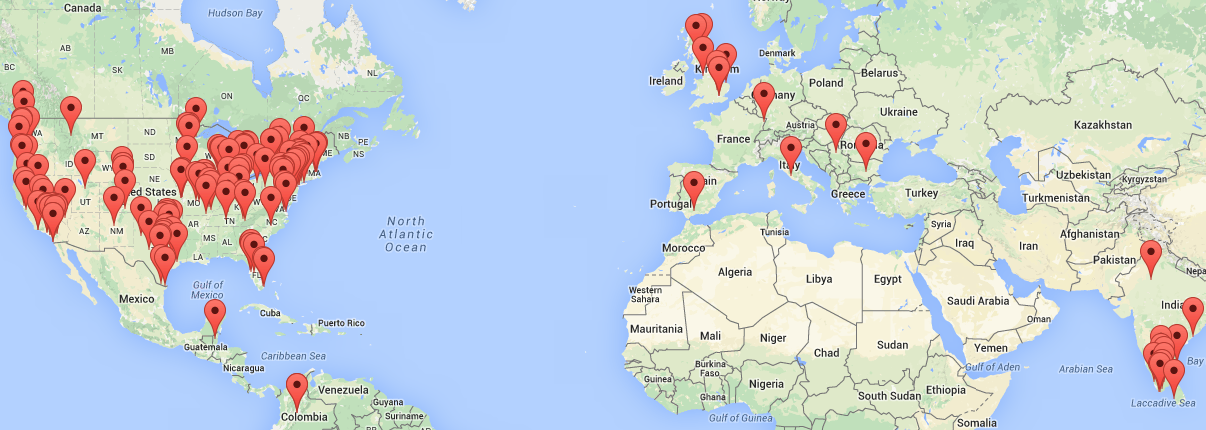
\includegraphics[width=\textwidth]{mapcities.png}
	\caption{Overview over the 149 cities chosen by subjects in Experiments 1, 3A and 3B.}
	\label{fig_map}
\end{figure}

List of cities in Experiment 1: \footnotesize{Albany, Albuquerque, Ames, Ann Arbor, Austin, Baltimore, Belgrade, Belmopan, Buffalo, Chennai, Chicago, Chico, Cincinnati, Corvallis, Cupertino, Denton, Denver, Dunmore, Fort Collins, Gobichettipalayam, Hampton, Klamath Falls, Kochi, Lakeland, Las Vegas, Los Angeles, Madurai, Miami, Minneapolis, Miramar, Mount Kisco, New York, Orange (FL), Pittsburgh, Pittsfield Charter Township, Potterville, Reno, Rome, San Angelo, San Bernardino, San Diego, Somerville, Springfield, Strasbourg, White Salmon, Williamsburg, Wilmington}.

\normalsize

List of cities in Experiment 3A: \footnotesize{Alameda, Austin, Beacon, Bedford, Belleville, Bellingham, Bengaluru, Berkeley, Bloomington, Boston, Bowie, Bowling Green (KY), Brooksville, Brownsville, Buffalo, Burlington, Cambridge, Camden, Cape Girardeau, Castlerock, Chicago, Cincinnati, College Station (TX), Colombo, Columbia, Denver, Desert Hot Springs (CA), Desoto, Duluth, Eastbrunswick, Edinburgh, Fairway, Farmersville, Fayetteville, Franklin, Germantown, Gettysburg, Glasgow, Goleta, Harwoodheights, Hemet, Highridge, Hollywood, Holt, Houston, Islavista, Jaipur, Karur, Keller, Lackawanna, Lake Oswego, Land O' Lakes, Lindsay, Little River-Academy (TX), Live Oak (TX), London, Lubbock, Marthandam, Mayfield, Minneapolis, Mission, Nagercoil, New York, Norridge, Orange, Overland Park (KA), Owensville, Palmsprings, Perryville, Pigeonforge, Poplarbluff, Portland, Poughkeepsie, Princeton, Provo, Revere, Rochester, Rochester Hills, Roeland Park, Salem, San Antonio, San Diego, Sanger, Savage, South Bend, Southport, Springboro, Springhill, St. Charles, Stony Brook (NY), St. Peters, Temple, Tirunelveli, Towson, Visakhapatnam, Warren, Weatherford, Wilmington, Xenia, Ypsilanti}.

\normalsize

List of cities in Experiment 3B: \footnotesize{Algonquin, Ashland, Chicago, Columbia, Jefferson City, Kansas City, Knoxville, Lexington, Linden, Medford, Minneapolis, Missoula, Mound, Overland Park, Portland, Seattle, Stara Zagora}.

\normalsize

\section{Exclusion of learning effects}

A possible criticism of our results could be the claim that the structure apparent from the recall protocol orderings is being learned by the subjects during the recall process, as opposed to being an inherent property of their long-term memory (LTM). Our analysis procedure assumes one consistent structure in LTM underlying the recall protocols; and excludes possible `outliers' using the jackknifing procedure (i.e. protocols which, when included, would statistically significantly change the resulting structure, are excluded from analysis).

If this assumption was incorrect, and subjects learned the structure during the experiment - or, alternatively, re-learned a different structure, then this would be apparent from the pattern of omitted recall protocols. Specifically, it would mean a significantly larger number of omitted early protocols compared to late protocols (the first, or first few protocols would be inconsistent with the learned structure more often than the last few).

To test whether this learning effect can be observed, we have tested the distributions of omitted recall protocols against the null hypothesis that the likelihood of omissions was uniform (just as likely to occur for the first few as for the last few protocols), using a chi-square test. The table below shows the results. 

For the real-world experiments, the null hypothesis cannot be rejected; thus, it is likely that there is no learning effect, and that our recall order paradigm indeed measures structures which have already been committed to LTM before the experiment. For the virtual reality experiment (Exp. 2), there seems to be some small non-uniformity, although not significant at $\alpha=0.01$. However, contrary to the objection that the structure arises from learning during the recall trials, early protocols were less likely \footnote{The frequency of omissions in Experiment 2 were: $1.1\%$ for the protocols presented first, $0.7 \%$ for those at position 2, $1.3\%$ at position 3, $1.6\%$ at position 4, $1.7\%$ at position 5, $1.9\%$ at position 6, and $1.8\%$ at position 7}, instead of more likely, to be excluded as outliers compared to late protocols. 

\begin{table}
	\centering
	\begin{tabularx}{\textwidth}{XXXX}
		\textbf{Exp. 1} & \textbf{Exp. 2} & \textbf{Exp. 3A}  & \textbf{Exp. 3B} \\ \hline
		$p=0.886 > 0.01$ & $p=0.015 > 0.01$ & $p=0.146 > 0.01$ & $p=0.495 > 0.01$  \\
		$c=2.339$ & $c=15.698$ & $c=9.538$ & $c=8.393$  \\ \hline
		%		\small{No evidence for \newline non-uniformity} & \small{Weak evidence for \newline non-uniformity} & \small{No evidence for \newline non-uniformity} & \small{No evidence for \newline non-uniformity} \\
	\end{tabularx}
	\caption{Results of chi-squared tests against the null hypothesis that there is no learning effect in the recall protocol data, i.e. that early recall protocols are as likely to be outliers than late recall protocols ($p$ is the p-value of the test; $c$ denotes the chi square test statistic). The non-significance of the results suggests that our recall order paradigm measures a property of long-term memory, and not something learned during the recall trials.}
	\label{tbl_chisq}
\end{table}

\section{Separability of co-represented and not co-represented building pairs}

The co-representation correlations reported in Section 3.3 of the main text raise hopes of straightforward predictability - what if a simple distance thresholding or linear decision boundary in the reported feature space is capable of fully explaining cognitive map structure, even for the random testing environments? Unfortunately, within sub-map and across sub-map building pairs are not linearly separable; and difficult to separate in general, even with complex state of the art classifiers. 

% (the Supplementary Information contains dimensionality-reduced plots of the pair distributions). We have tried several state of the art classification algorithms from machine learning, including kernel Support Vector Machines and Random Forests.

\begin{figure}[h]
	\centering
	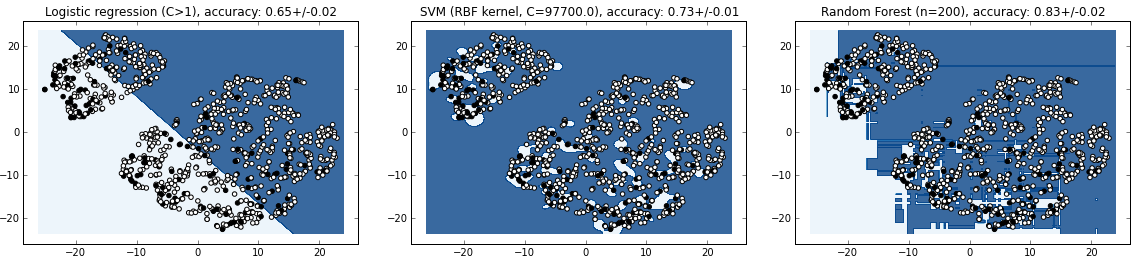
\includegraphics[width=\textwidth]{exp2class.png}
	\caption{Pairs of buildings in the space of all features, and their separability according to co-representation, in Experiment 2 using three different classifiers: logistic regression (left), Support Vector Machine with RBF-kernel (middle) and Random Forest (right). Each point represents a building pair (filled black if both buildings lie on the same sub-map, and white if they do not), with its position being a two-dimensional projection of the full six-dimensional feature space using t-SNE.  Although 2D decision boundaries are visualized, the reported classifier accuracies were obtained in the original feature space, using 10-fold cross validation and after hyperparameter optimization.}
	\label{fig_classify}
\end{figure}

Figure \ref{fig_classify} shows the distances of all pairs of buildings in all features in Experiment 2, normalized by dividing each feature by its standard deviation for each participant map, and compressed down to two-dimensional space for visualization using t-SNE \citep{van2008visualizing} (without normalization across buildings of each map, classifiers are unable to perform above chance). Apart from the building pairs (which concentrate into two groups according to function - shops and houses), decision boundaries obtained with three different classifiers are also plotted. Although there is a trend of building pairs being more likely to be on the same sub-map when closer together (higher concentration of same-map pairs towards the lower left), the data is clearly not well-separable. As can be seen from this Figure, accurate prediction of full subject map structures - or even whether single building pairs belong to the same sub-map - using simple classification is impossible using naive approaches. More complex machine learning algorithms such as random forests (state-of-the art classifiers based on ensembles of decision trees) \citep{breiman2001random} can predict for around $83 \%$ of building pairs whether they belong to the same representation (note that the accuracies were obtained by classifying the full high-dimensional data set, not just the 2D projection plotted in Figures \ref{fig_classify} and \ref{fig_classify_rl}). However, the map structures collected in our experiments contain $10$ and $28$ pairs (in the $5$-building and $8$-building maps), which would make the probability of full map structures - all pairs - being predicted correctly using this approach $15.5 \%$ and $0.5 \%$ respectively (the situation is even worse in real-world environments, as can be seen in the next section).

\begin{figure}[h]
	\centering
	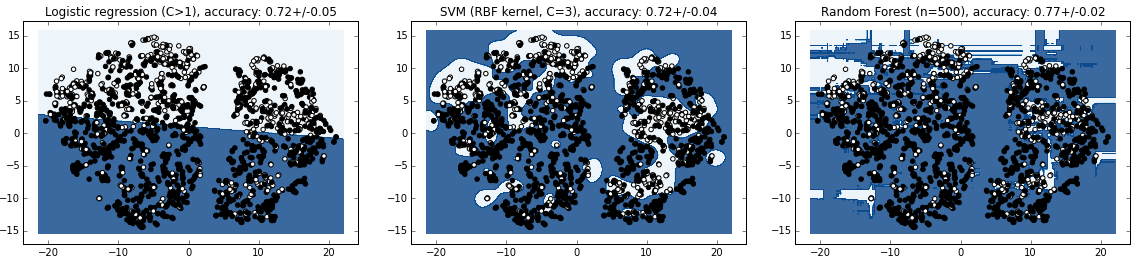
\includegraphics[width=\textwidth]{exp3Aclass.png}
	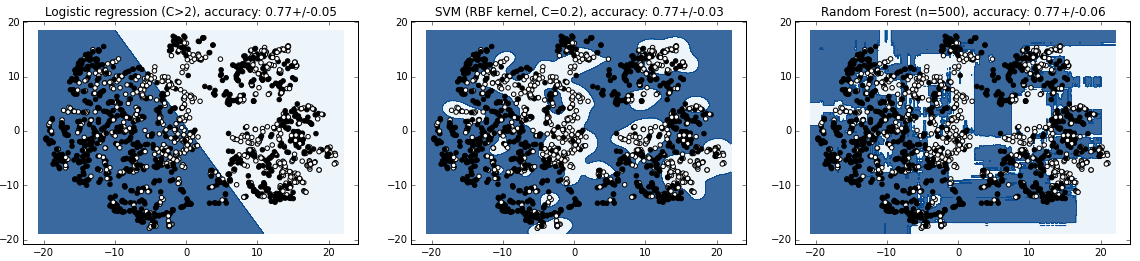
\includegraphics[width=\textwidth]{exp3Bclass.png}
	\caption{Pairs of buildings in the space of all features, and their separability according to co-representation, in Experiment 3 using three different classifiers: logistic regression (left), Support Vector Machine with RBF-kernel (middle) and Random Forest (right). Top: Condition A. Bottom: Condition B}
	\label{fig_classify_rl}
\end{figure}

In the more complex real-world setting of Experiment 3, separating pairs of buildings which belong to the same sub-map and those belonging to different sub-maps is even more difficult than in virtual reality environments, as shown by Figure \ref{fig_classify_rl} and evidenced by the lower accuracies obtained after 10-fold cross validation. This Figure shows the distances of all pairs of buildings in all features, normalized by dividing each feature by its standard deviation for each participant map, and compressed down to two-dimensional space for visualization using t-SNE \citep{van2008visualizing}. Note that the Figure shows prediction accuracies of pairs of buildings (whether or not a pair was represented on the same sub-map), and not of entire map structures. To correctly predict a map structure, all pairs within would need to be predicted correctly. Given the $77 \%$ accuracy of the best classifier in Figure \ref{fig_classify_rl}, correct predictions based on classification are even more unlikely than in Experiment 2 ($0.77^{5 \choose 2}=7.3 \%$ in condition A, and $0.77^{8 \choose 2}=0.0 \%$ in condition B).

%Due to the large number of trees - $N=200$ -, this approach is able to learn decision trees describing regions in this feature space for each individual participant, which is why it performs better than the other approaches.


%\footnote{Logistic regression performed equally with l1 and l2 regularization, and with any regularization parameter C greater than 1}

%The observation that building pair classification fails altogether \footnote{All approaches yield accuracies around $50\%$ for binary, within vs. between sub-map classification for unnormalized data} when distances are not normalized across buildings of each map (within each subject and environment) provides an important hint as to the reason of why classification is a sub-optimal approach to model and predict cognitive map structure. It implies that \textit{relative} distances are much more relevant than absolute distances. This is another argument in favour of the clustering hypothesis, since in clustering, relative distances are the sole criterion of cluster structure. Furthermore, it illustrates the difficulty of the problem, and the inadequacy of naive approaches for solving it.

%\documentclass[12pt,PhD,twoside]{muthesis}
%\usepackage{verbatim}
%\usepackage{graphicx}
%\graphicspath{ {img/} }
%\usepackage{url} % typeset URL's reasonably
%\usepackage{listings}
%\usepackage{pdfpages}
%\usepackage{tabu}
%\usepackage{longtable}
%\usepackage{multirow, tabularx}
%\usepackage[labelfont=bf]{caption}
%\usepackage{natbib}
%\usepackage{pslatex} % Use Postscript fonts
%\usepackage{amsmath}
%\usepackage{amssymb}
%\usepackage{bm}
%\usepackage{pseudocode}
%\DeclareMathOperator*{\argmin}{arg\,min}
%\DeclareMathOperator*{\argmax}{arg\,max}
%\def\approxprop{%
%	\def\p{%
%		\setbox0=\vbox{\hbox{$\propto$}}%
%		\ht0=0.6ex \box0 }%
%	\def\s{%
%		\vbox{\hbox{$\sim$}}%
%	}%
%	\mathrel{\raisebox{0.7ex}{%
%			\mbox{$\underset{\s}{\p}$}%
%		}}%
%	}
%\begin{document}
%\bibliographystyle{model5-names}

%\chapter[Probabilistic neural models and their plausibility]{Neural implementations of uncertainty and inference and their consistency with the hippocampal complex}

\chapter{Supplementary Information for Chapter 6}
\label{apx:lidaspm}
\section{Comparison of hierarchical activation gradient-based route planning with human performance on the TSP task}


In order to evaluate the plausibility of gradient-based multi-goal route planning, as described in the main text (see Figure 5), we have used data collected from participants recruited on Amazon Mechanical Turk, tasked with solving the travelling salesperson problem (TSP) in virtual reality environments. Data from 46 participants was analysed here. They were asked to mark all buildings in the 3D environment and then return to the building they started out with, using the shortest path possible (see (Madl et al., 2013) for details). 

Each participant performed 5 trials in each of three types of environments: random (in which buildings were randomly distributed), clustered by looks (in which buildings of the same type, e.g. churches, were ensured to be grouped, close to each other), and clustered by distance (in which some buildings were placed close to build groups, regardless of their visual similarity).

Figure \ref{tsp} shows participant performance, compared with a gradient-based route planner operating on a flat (single-level) representation. Interestingly, this non-hierarchical model seems to explain the human data well. As a caveat, it should be mentioned that participants were not checked for prior experience with 3D environments (an unknown percentage may have had trouble with the controls, falling back to the simplest strategy). Furthermore, this task is inherently more difficult in virtual reality, where cues important in real-world navigation are not available (e.g. depth information from stereo disparity, path integration / self movement information, etc.).

To avoid these caveats, we have replicated a real-world TSP experiment by (Wiener et al., 2009). This experiment was performed in a $6.0m$ x $8.4m$ room, with $25$ different locations marked by boxes with symbols on them, as illustrated in Figure \ref{tsp2}A. Subjects were given a `shopping list' containing a number of different symbols, each of which denoted a location that they had to visit, and they subsequently had to plan the shortest route visiting all of these locations. Figure \ref{tsp2} shows subjects' performance at this task, and compares it with the simulated performance of an agent using the gradient climbing heuristic on two-level hierarchical cognitive map. The models performance closely  accounts for human data, as  can  be  seen  from  this  figure,  which  substantiates  the  models  cognitive plausibility.


\begin{figure}[!ht]
	\begin{center}
		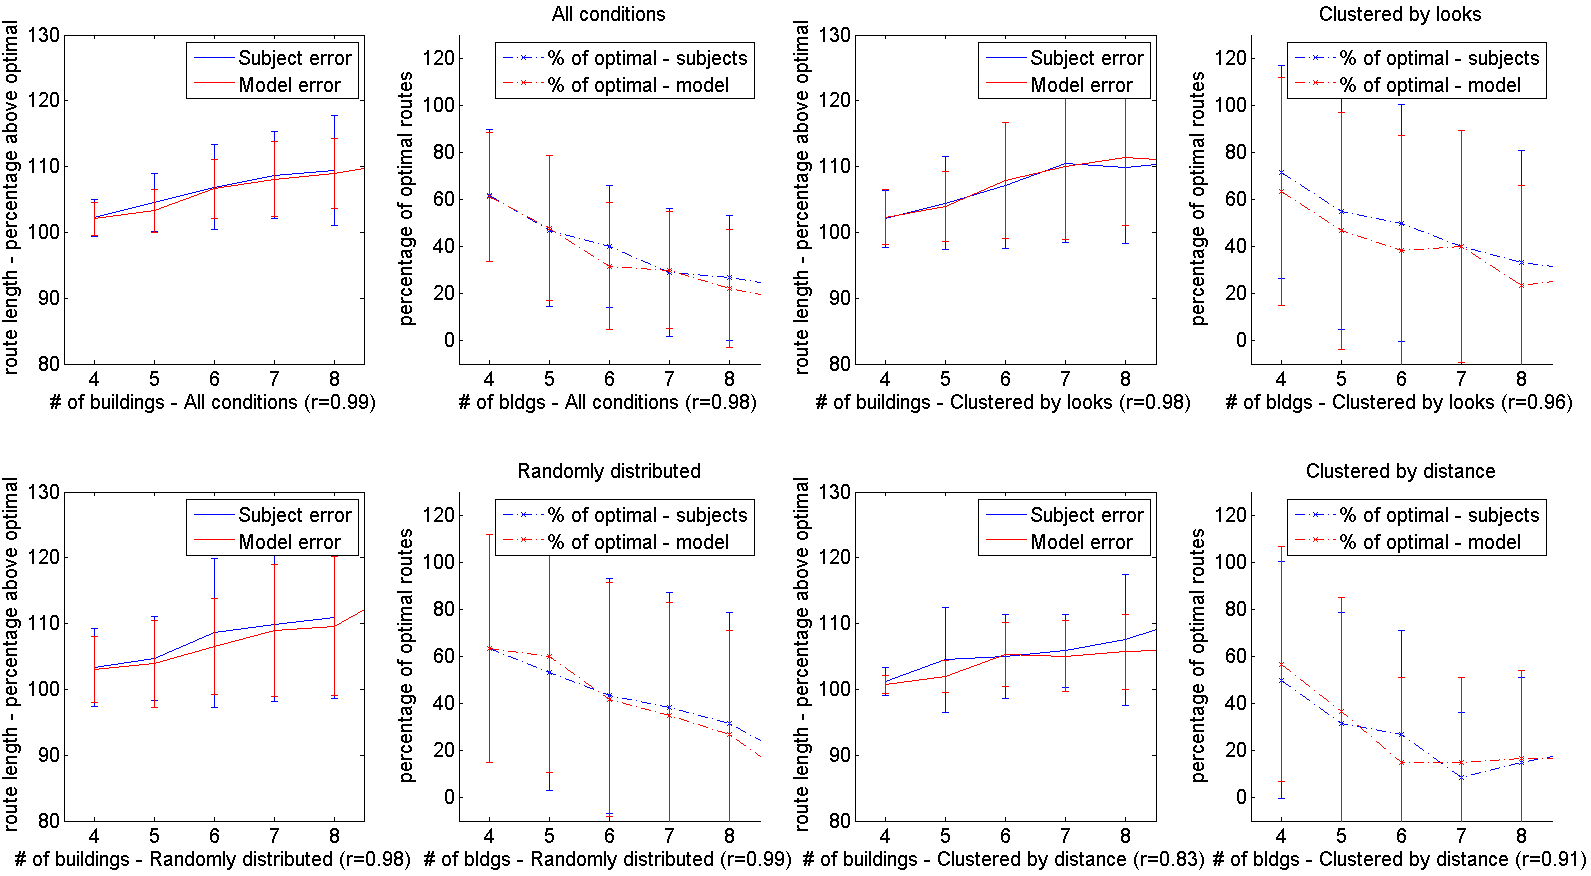
\includegraphics[width=\textwidth]{img/tsperrors2}
	\end{center}
	\caption[Human performance in virtual reality, compared to gradient-based planning]{
		{\bf Human performance in virtual reality, compared to gradient-based planning} on a flat grid of place nodes. 
	}
	\label{tsp}
\end{figure}

\begin{figure}[!ht]
	\begin{center}
		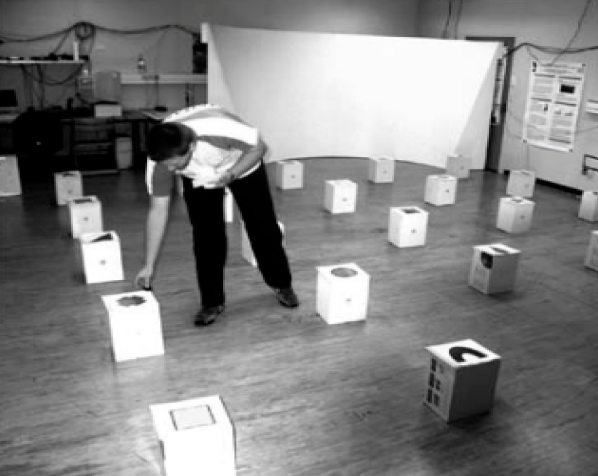
\includegraphics[width=0.49\textwidth]{img/wienerexp}
		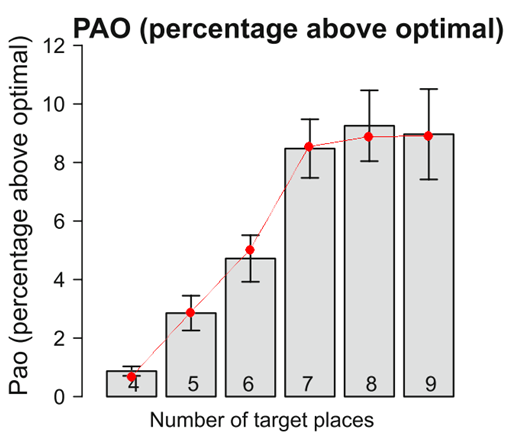
\includegraphics[width=0.49\textwidth]{img/wieneretal2009_spatial_tsp_comparison.png}
	\end{center}
	\caption[Human performance in a real-world experiment]{
		{\bf Human performance in a real-world experiment (Wiener et al., 2009), compared to gradient-based planning,} on a hierarchical grid of place nodes. Figures modified from (Wiener et al., 2009) with permission.
	}
	\label{tsp2}
\end{figure}


%An appendix is just like any other chapter, except that it comes after
%the appendix command in the master file.
%
%One use of an appendix is to include an example of input to the system
%and the corresponding output.
%
%One way to do this is to include, unformatted, an existing input file. 
%You can do this using \verb=\verbatiminput=. In this appendix we
%include a copy of the C file \textsf{hello.c} and its output file
%\textsf{hello.out}. If you use this facility you should make sure that
%the file which you input does not contain \texttt{TAB} characters,
%since \LaTeX\ treats each \texttt{TAB} as a single space; you can use
%the Unix command \texttt{expand} (see manual page) to expand tabs into
%the appropriate number of spaces. 
%
%\section{Example input and output}
%\label{sec:inp-eg}
%\subsection{Input}
%\label{sec:input}
%(Actually, this isn't input, it's the source code, but it will do as
%an example)
%
%\verbatiminput{hello.c}
%
%\subsection{Output}
%\label{sec:output}
%
%\verbatiminput{hello.out}
%\subsection{Another way to include code}
%You can also use the capabilities of the \texttt{listings} package to
%include sections of code, it does some keyword highlighting.
%
%\lstinputlisting[language=C]{hello.c}

%
%\begin{thebibliography}{2}
%	\expandafter\ifx\csname natexlab\endcsname\relax\def\natexlab#1{#1}\fi
%	\providecommand{\url}[1]{\texttt{#1}}
%	\providecommand{\href}[2]{#2}
%	\providecommand{\path}[1]{#1}
%	\providecommand{\DOIprefix}{doi:}
%	\providecommand{\ArXivprefix}{arXiv:}
%	\providecommand{\URLprefix}{URL: }
%	\providecommand{\Pubmedprefix}{pmid:}
%	\providecommand{\doi}[1]{\href{http://dx.doi.org/#1}{\path{#1}}}
%	\providecommand{\Pubmed}[1]{\href{pmid:#1}{\path{#1}}}
%	\providecommand{\bibinfo}[2]{#2}
%	\ifx\xfnm\relax \def\xfnm[#1]{\unskip,\space#1}\fi
%	%Type = Inproceedings
%	\bibitem[{Madl et~al.(2013)Madl, Franklin, Chen \& Trappl}]{madl2013spatial}
%	\bibinfo{author}{Madl, T.}, \bibinfo{author}{Franklin, S.},
%	\bibinfo{author}{Chen, K.}, \& \bibinfo{author}{Trappl, R.}
%	(\bibinfo{year}{2013}).
%	\newblock \bibinfo{title}{Spatial working memory in the lida cognitive
%		architecture}.
%	\newblock In {\it \bibinfo{booktitle}{Proc. international conference on
%			cognitive modelling}\/}.
%	%Type = Article
%	\bibitem[{Wiener et~al.(2009)Wiener, Ehbauer \& Mallot}]{Wiener2009}
%	\bibinfo{author}{Wiener, J.~M.}, \bibinfo{author}{Ehbauer, N.~N.}, \&
%	\bibinfo{author}{Mallot, H.~a.} (\bibinfo{year}{2009}).
%	\newblock \bibinfo{title}{{Planning paths to multiple targets: memory
%			involvement and planning heuristics in spatial problem solving.}}
%	\newblock {\it \bibinfo{journal}{Psychological research}\/},  {\it
%		\bibinfo{volume}{73}\/}, \bibinfo{pages}{644--58}.
%	\DOIprefix\doi{10.1007/s00426-008-0181-3}.
%	
%\end{thebibliography}




%\bibliography{lidaspm}

%\end{document}
%\chapter[Probabilistic neural models and their plausibility]{Neural implementations of uncertainty and inference and their consistency with the hippocampal complex}

\chapter{Additional evidence for sampling-based Bayesian localization}
\label{apx:pfev}

In Chapter 7, we have addressed the observation that there is a subset of neurons in the hippocampus with firing fields which seem to contradict the uncertainty predictions of a Bayesian model. The reasonably god fit to place fields sizes reported in Chapter 4, although imperfect, suggest that some place cells do approximate Bayesian posteriors. However, it is very likely that only a subset does so, and that part of the hippocampus performs different computations altogether.

To show that our sampling-based Bayesian localization model can function even under conditions where a proportion of the samples is corrupted by non-Bayesian processes, we have compared the distribution of uncertainties predicted by the sampling-based model to the distribution of place field sizes.

We have used the implemented sampling-based cognitive model (described in Chapter 6) to replicate the experiment (Burke et al., 2011). In the experiment, rats were running in circles on a circular track with 106cm diameter, which contained 2 food trays to motivate the rats, and no objects in one condition and 8 pseudorandomly distributed, different objects in another condition. The model performed random trajectories in an environment of the same proportions, with the same landmarks. 

Figure \ref{distr} shows the resulting distribution of uncertainties along the track, measured as the standard deviation of all posterior samples (location hypotheses) in the model. These uncertainties are compared to the distribution of place field sizes along the track. Note the matching ratio of the most frequent place field sizes and uncertainties at $21cm$ (objects) and $38cm$ (no objects) respectively, and the roughly matching ratio between all normalized frequencies of occurrence between objects and no objects conditions.

\begin{figure}[!ht]
	\begin{center}
		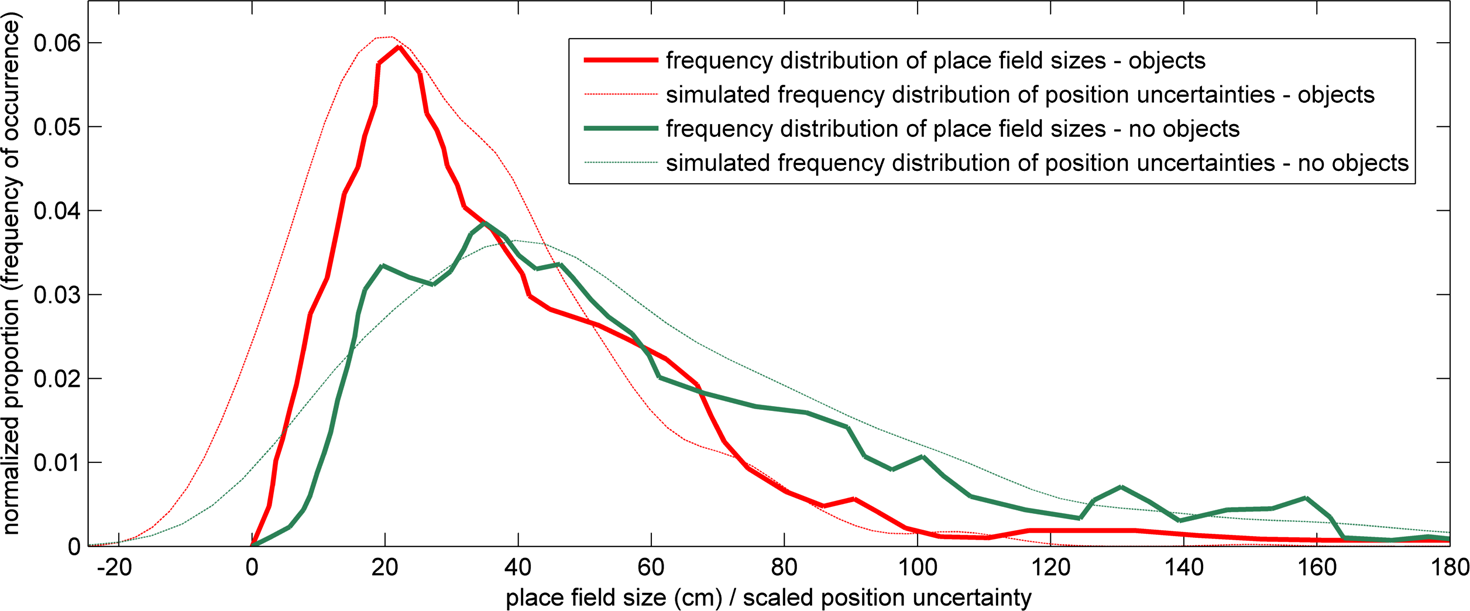
\includegraphics[width=\textwidth]{img/burkefreqdist}
	\end{center}
	\caption[Occurrence frequencies of different place field sizes compared to those of position uncertainties in the model]{
		{\bf Occurrence frequencies of different place field sizes} in all measured neurons in the no
		objects (blue) and 8 objects (red) conditions, compared to the frequencies of position uncertainties in
		the simulation. Data from (Burke et al., 2011). 
	}
	\label{distr}
\end{figure}



%An appendix is just like any other chapter, except that it comes after
%the appendix command in the master file.
%
%One use of an appendix is to include an example of input to the system
%and the corresponding output.
%
%One way to do this is to include, unformatted, an existing input file. 
%You can do this using \verb=\verbatiminput=. In this appendix we
%include a copy of the C file \textsf{hello.c} and its output file
%\textsf{hello.out}. If you use this facility you should make sure that
%the file which you input does not contain \texttt{TAB} characters,
%since \LaTeX\ treats each \texttt{TAB} as a single space; you can use
%the Unix command \texttt{expand} (see manual page) to expand tabs into
%the appropriate number of spaces. 
%
%\section{Example input and output}
%\label{sec:inp-eg}
%\subsection{Input}
%\label{sec:input}
%(Actually, this isn't input, it's the source code, but it will do as
%an example)
%
%\verbatiminput{hello.c}
%
%\subsection{Output}
%\label{sec:output}
%
%\verbatiminput{hello.out}
%\subsection{Another way to include code}
%You can also use the capabilities of the \texttt{listings} package to
%include sections of code, it does some keyword highlighting.
%
%\lstinputlisting[language=C]{hello.c}

%\bibliography{refs}
%%\chapter[Probabilistic neural models and their plausibility]{Neural implementations of uncertainty and inference and their consistency with the hippocampal complex}

\chapter{Preliminary experiments and negative results}
\label{apx:prelimneg}



%An appendix is just like any other chapter, except that it comes after
%the appendix command in the master file.
%
%One use of an appendix is to include an example of input to the system
%and the corresponding output.
%
%One way to do this is to include, unformatted, an existing input file. 
%You can do this using \verb=\verbatiminput=. In this appendix we
%include a copy of the C file \textsf{hello.c} and its output file
%\textsf{hello.out}. If you use this facility you should make sure that
%the file which you input does not contain \texttt{TAB} characters,
%since \LaTeX\ treats each \texttt{TAB} as a single space; you can use
%the Unix command \texttt{expand} (see manual page) to expand tabs into
%the appropriate number of spaces. 
%
%\section{Example input and output}
%\label{sec:inp-eg}
%\subsection{Input}
%\label{sec:input}
%(Actually, this isn't input, it's the source code, but it will do as
%an example)
%
%\verbatiminput{hello.c}
%
%\subsection{Output}
%\label{sec:output}
%
%\verbatiminput{hello.out}
%\subsection{Another way to include code}
%You can also use the capabilities of the \texttt{listings} package to
%include sections of code, it does some keyword highlighting.
%
%\lstinputlisting[language=C]{hello.c}

\chapter[Evaluation of the ADP-GDA metric]{Performance of the ADP-GDA metric on constrained clustering benchmarks}
\label{apx:adsmetric}

\section*{Introduction}

We have proposed a novel approach for learning a metric for clustering with pairwise constraints in Section 2.5.2 and have used it to model human spatial representation structure in Chapter 5, showing that it can help predict whether buildings are co-represented (belong to the same sub-map in spatial memory) in a large majority of cases. Here, we briefly summarize the difference of this approach from other metric learning methods, and present some preliminary results of its performance compared to state of the art approaches.

The framework using a generative classifier as a distance function can be seen as a novel approach to perform non-linear metric learning using weak supervision in the form of pairwise constraints, in order to improve clustering performance, as pioneered in its linear form by \citep{xing2002distance}. Although this problem is very similar to metric learning in general, the criterion of interest is often somewhat different: as opposed to optimizing the performance of some classifier as in e.g. \citep{bellet2012similarity}), or for a large margin as in e.g. \citep{weinberger2005distance}, the goal is ensuring that all instances of a cluster are closer under the learned metric than those of different clusters. 

For general applicability, non-linear metrics are vital, because of the problem of \textit{multimodality}. When data points forming several groups or `modes' in unweighted feature space actually belong to the same cluster semantically, as indicated by ML constraints, there exists no linear projection able to separate them, and linear methods must inevitably fail. A traditional example is the XOR dataset, consisting of four groups, connected by diagonal ML constraints, such that there exists no linear separating hyperplane - see Figure \ref{fig:motivation2}a. 

Although kernel-based methods can deal with multimodal clustering problems (or any complicated data distribution) according to the Representer Theorem, in theory, given the optimal kernel and suitable parameters, in practice it is often difficult to find such a kernel. Most non-linear metric learning methods able to learn suitable kernels are sensitive to multiple hyperparameters, and, being nonconvex optimization problems, frequently get stuck in local minima.

A further issue with popular isotropic kernels such as the Radial Basis Function (RBF), frequently used in non-linear metric learning \citep{baghshah2010kernel, chitta2011approximate}, is that they are ill-suited for data with features on very different scales, since the optimal regularization parameters in one dimension can be suboptimal in other dimensions in this case, as pointed out by \citep{ong2005learning} (who propose a solution only in the supervised setting). 

\begin{figure*}[t]
	\centering
	
	\subfloat[XOR dataset]{%
		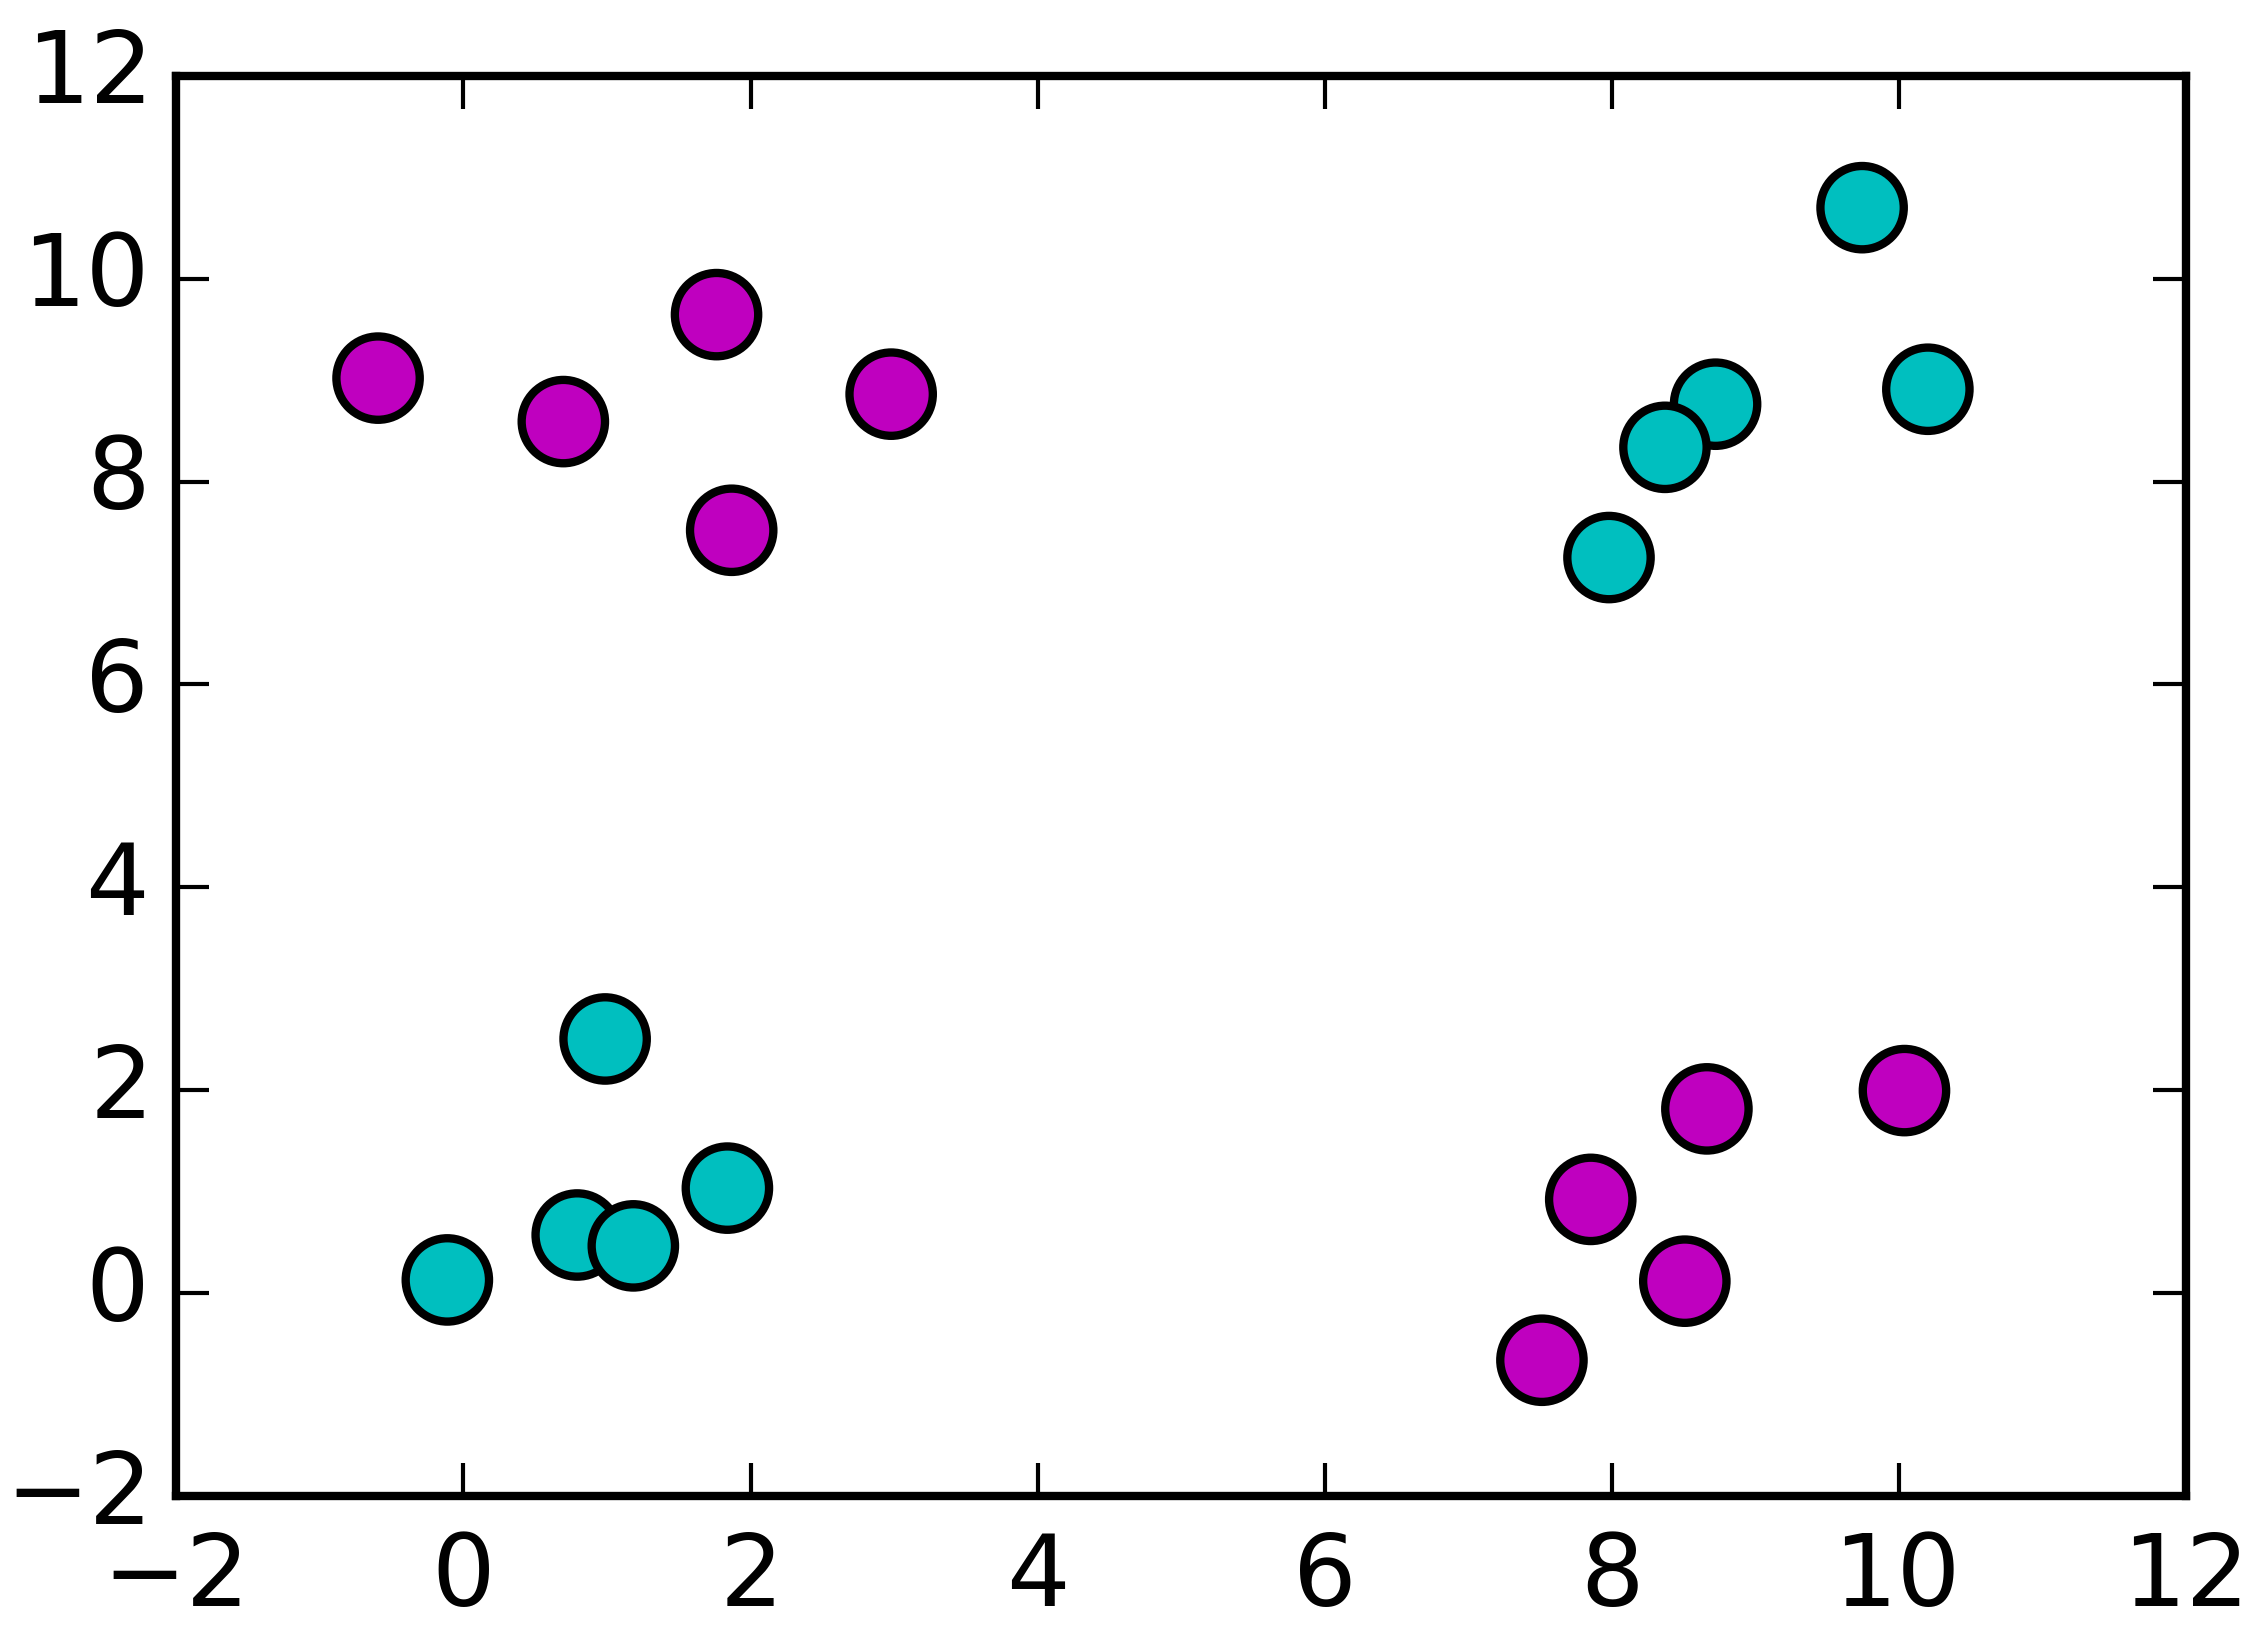
\includegraphics[width=0.25\textwidth]{quadplot1}%
	}
	\subfloat[Pairwise differences]{%
		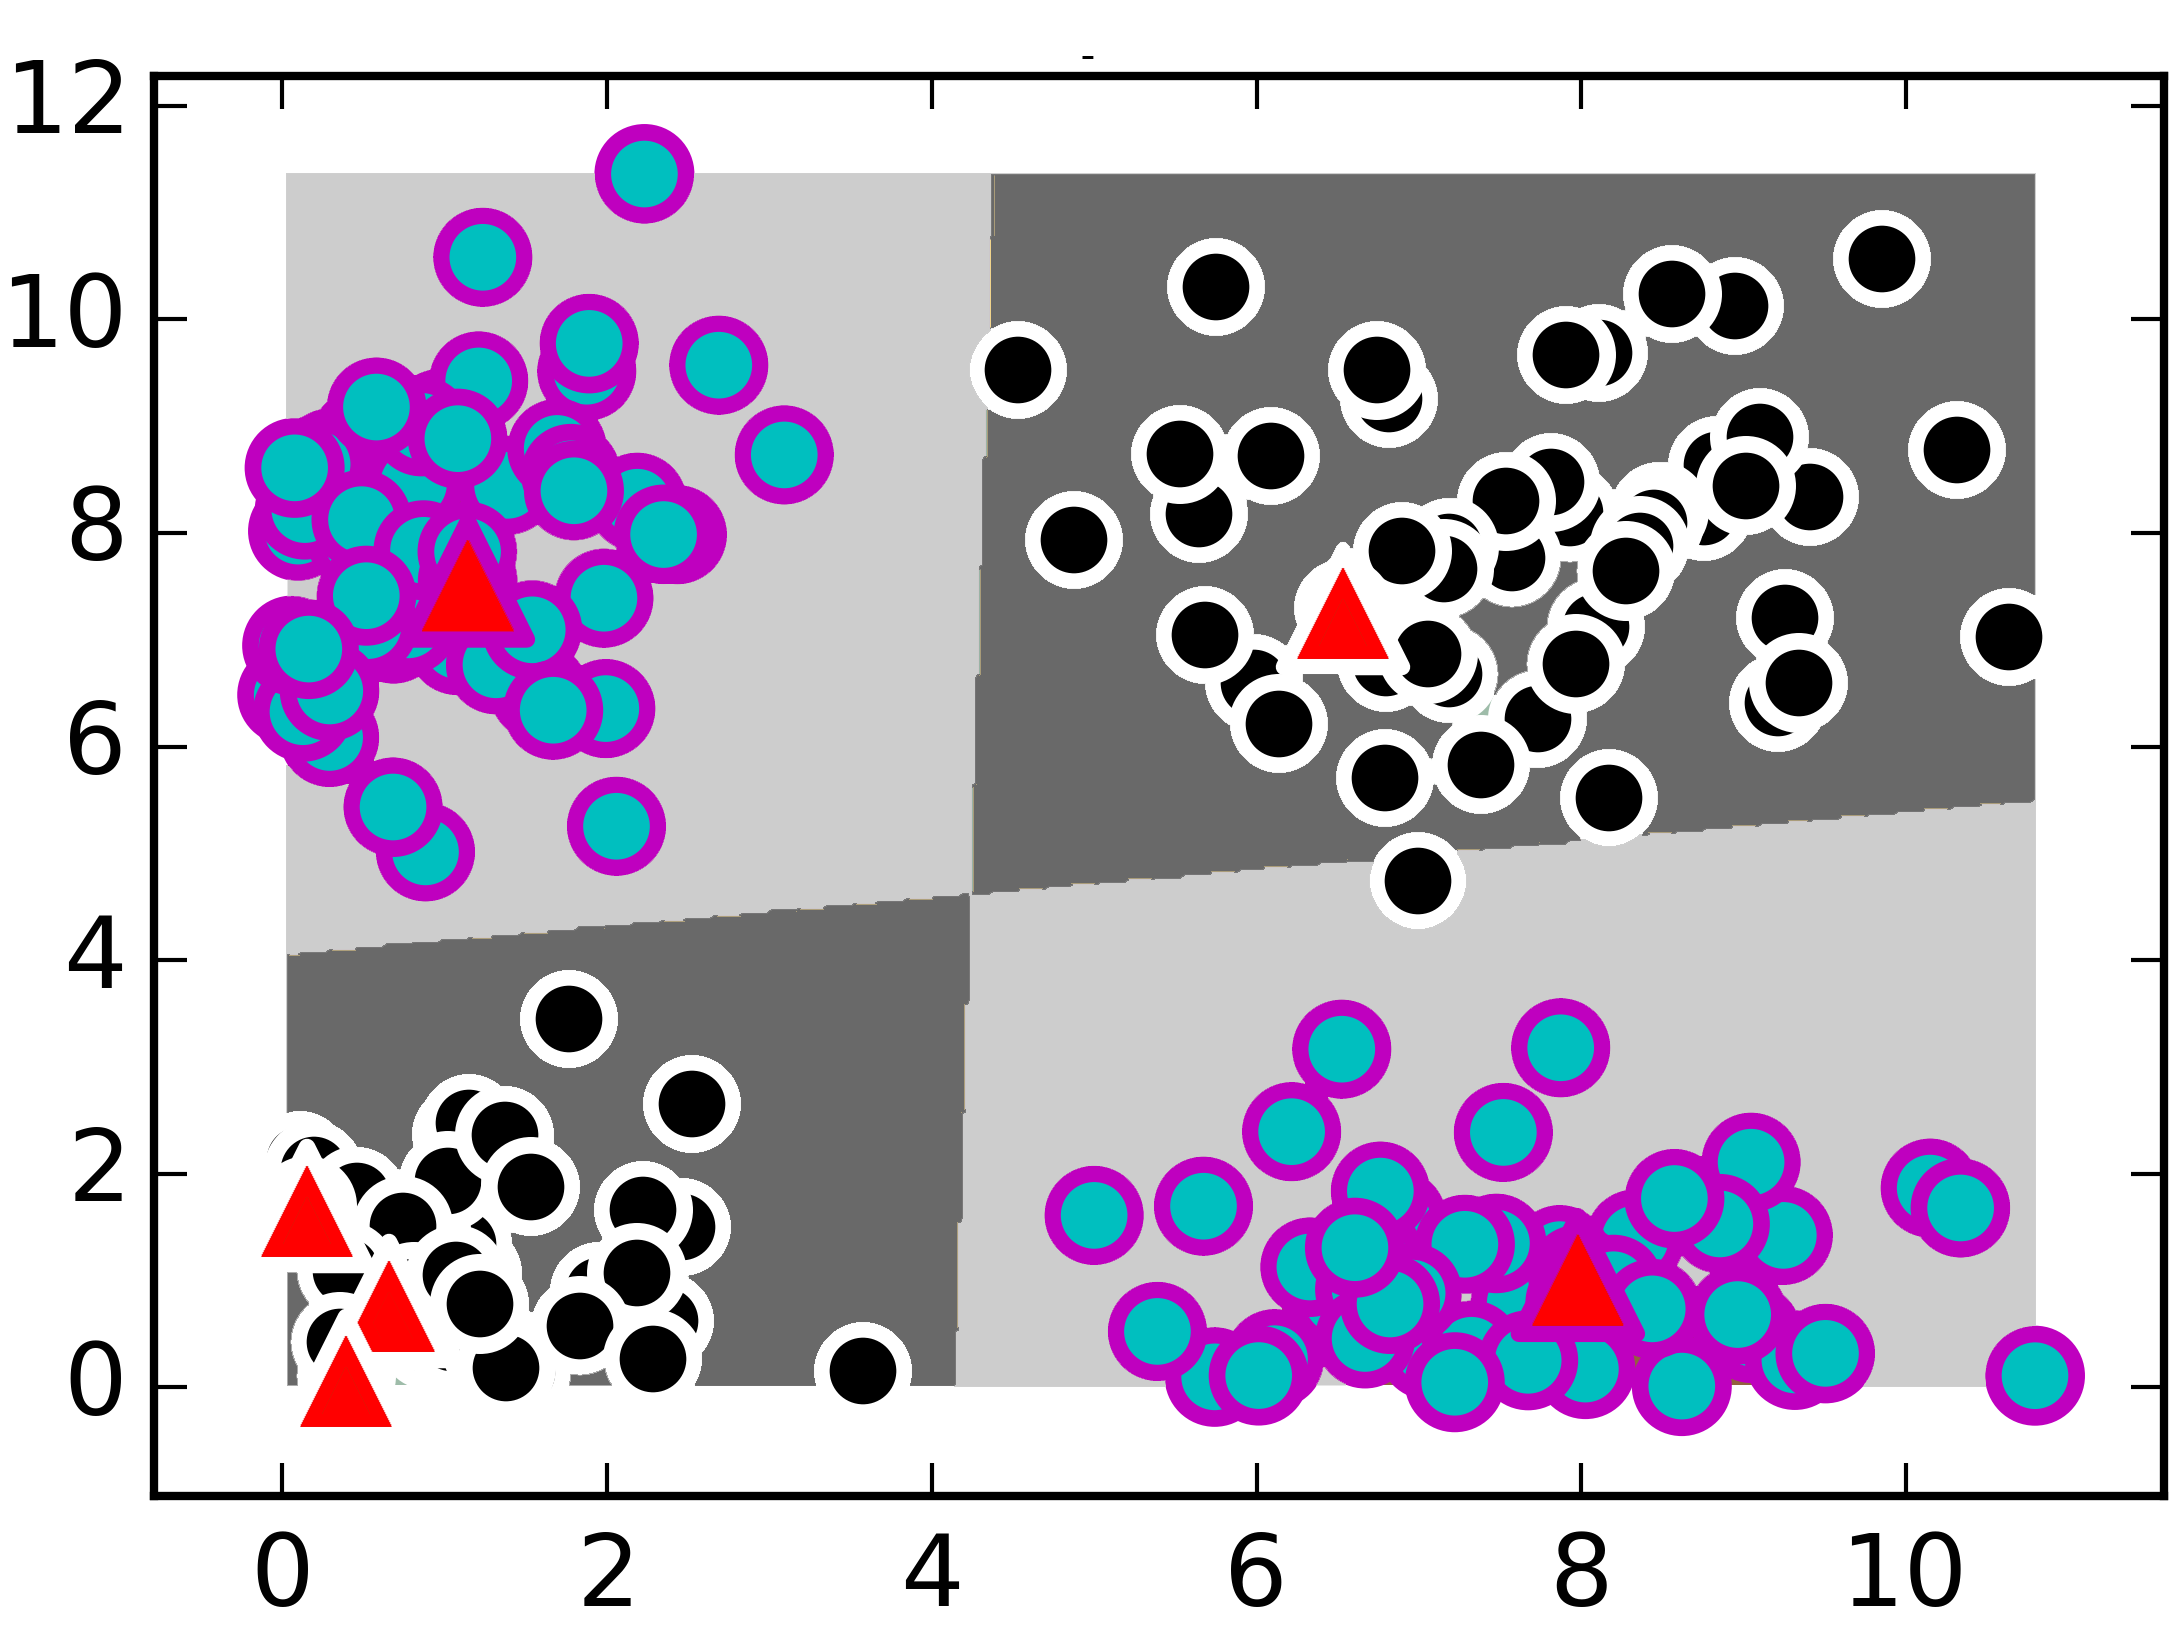
\includegraphics[width=0.25\textwidth]{quadplot2}%
	}
	\subfloat[Non-isotropic data]{%
		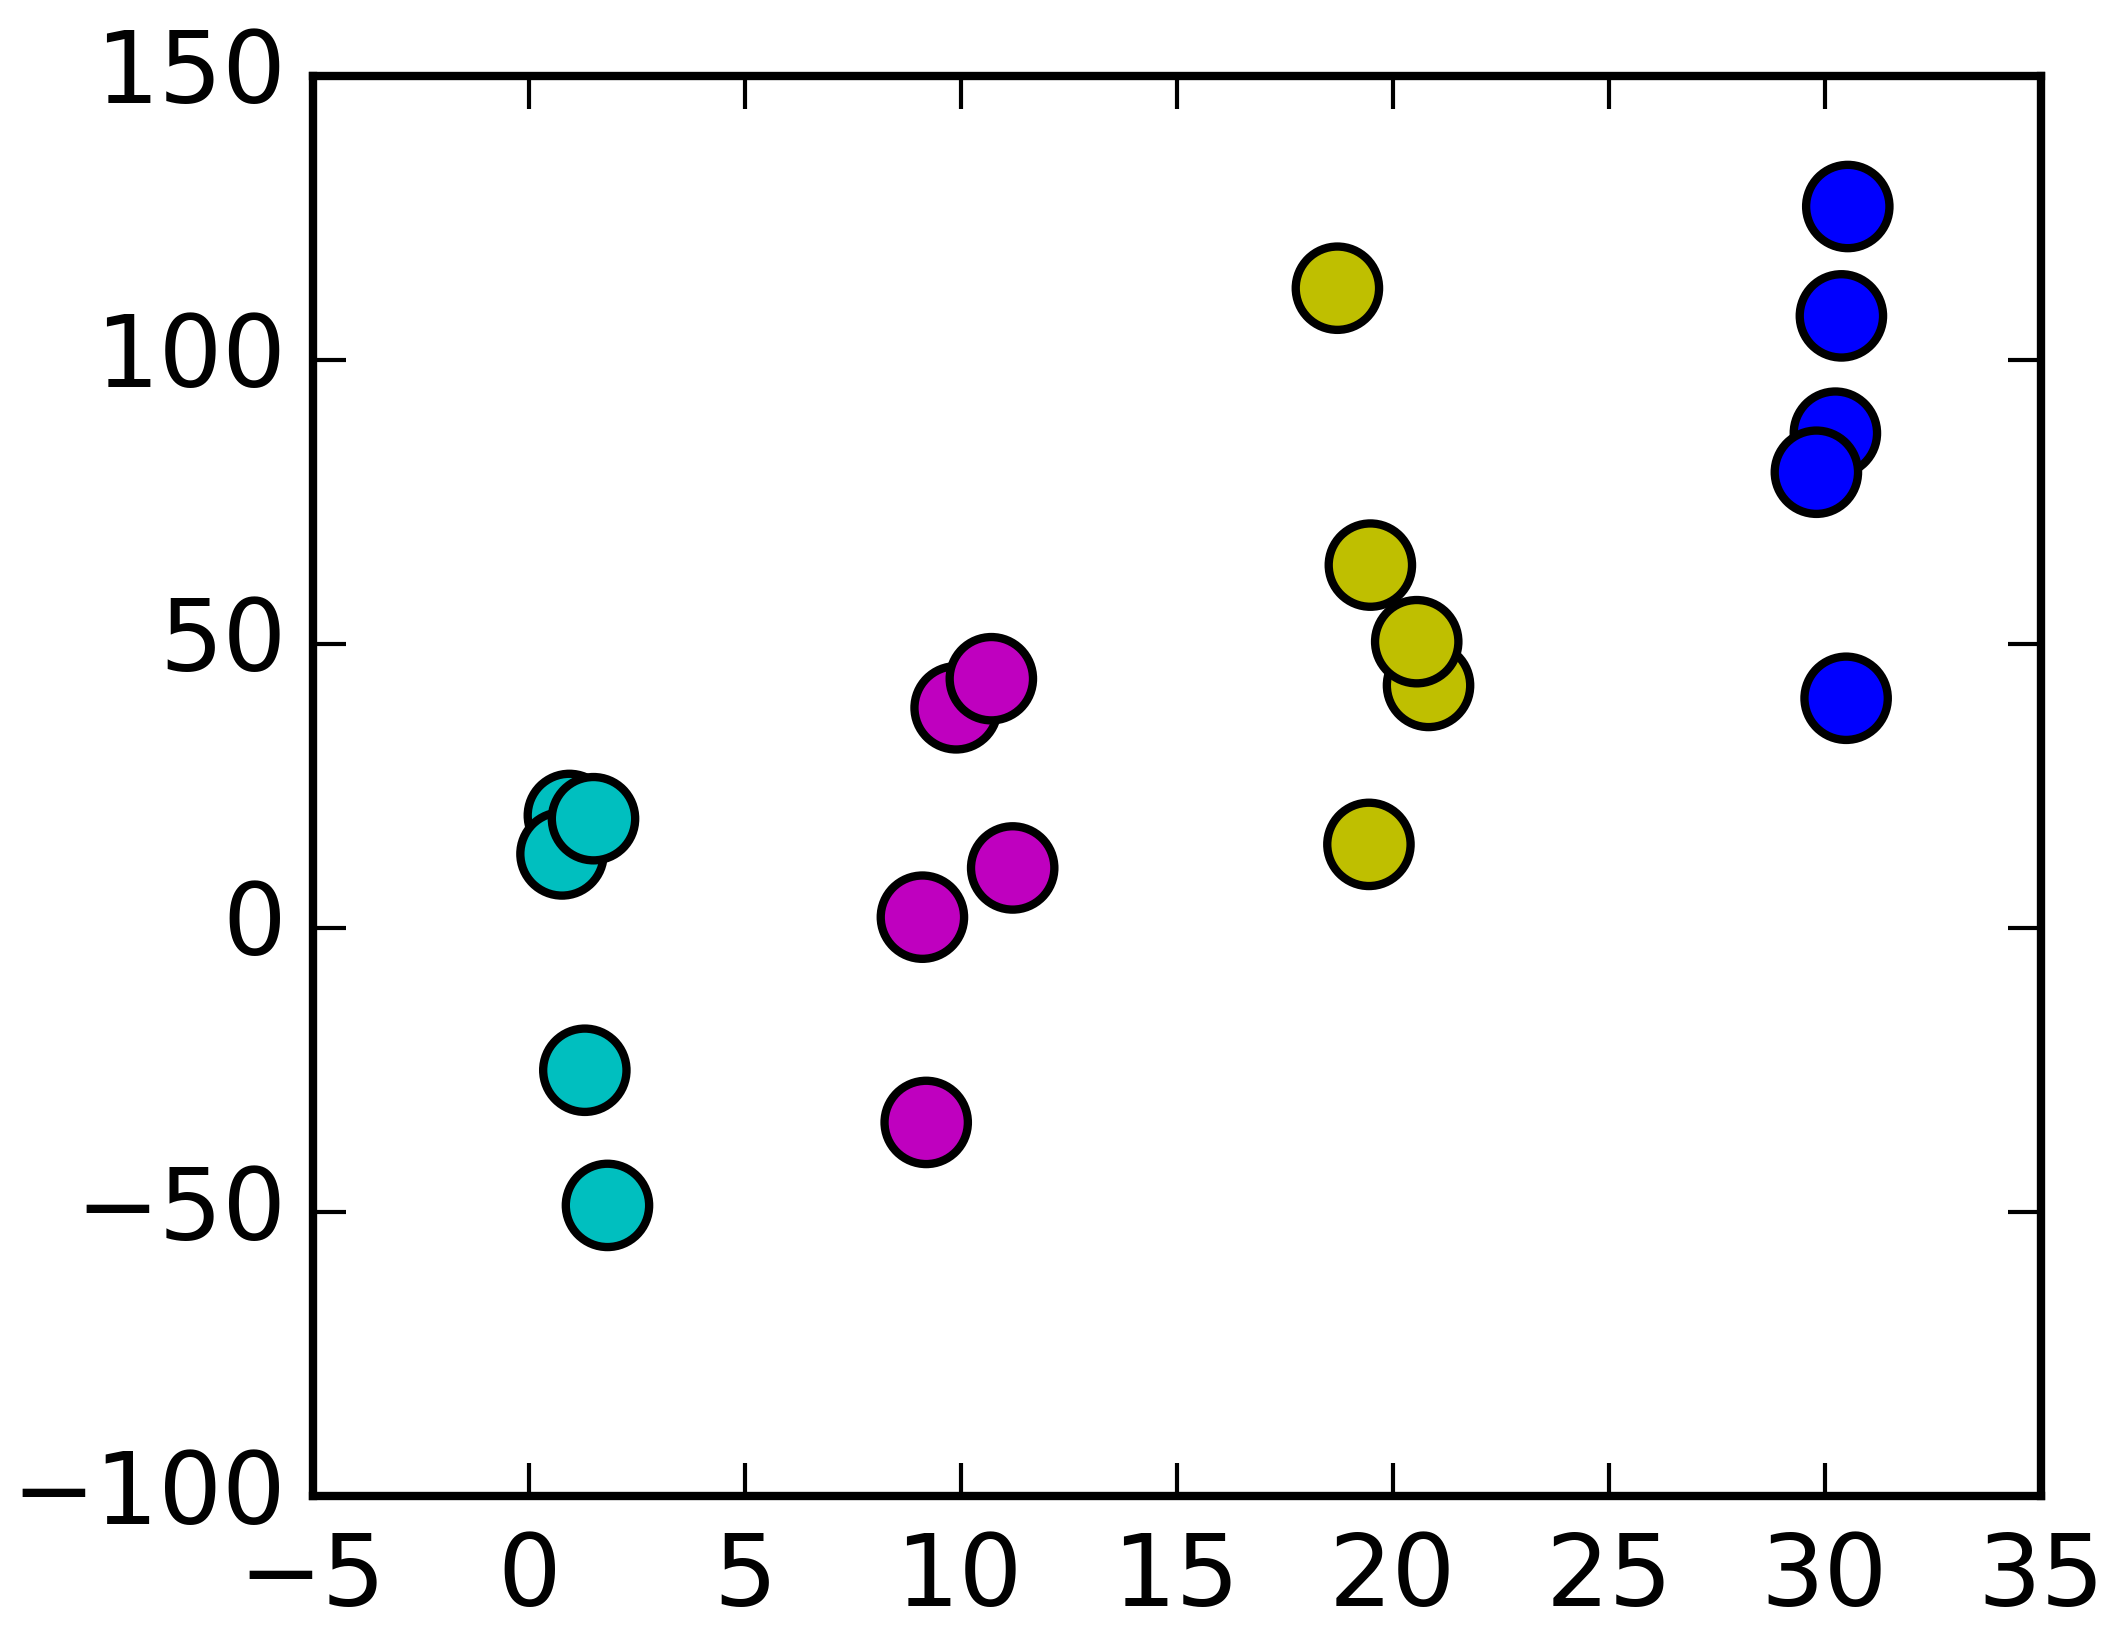
\includegraphics[width=0.25\textwidth]{isosvmproblem1}%
	}
	\subfloat[Pairwise differences]{%
		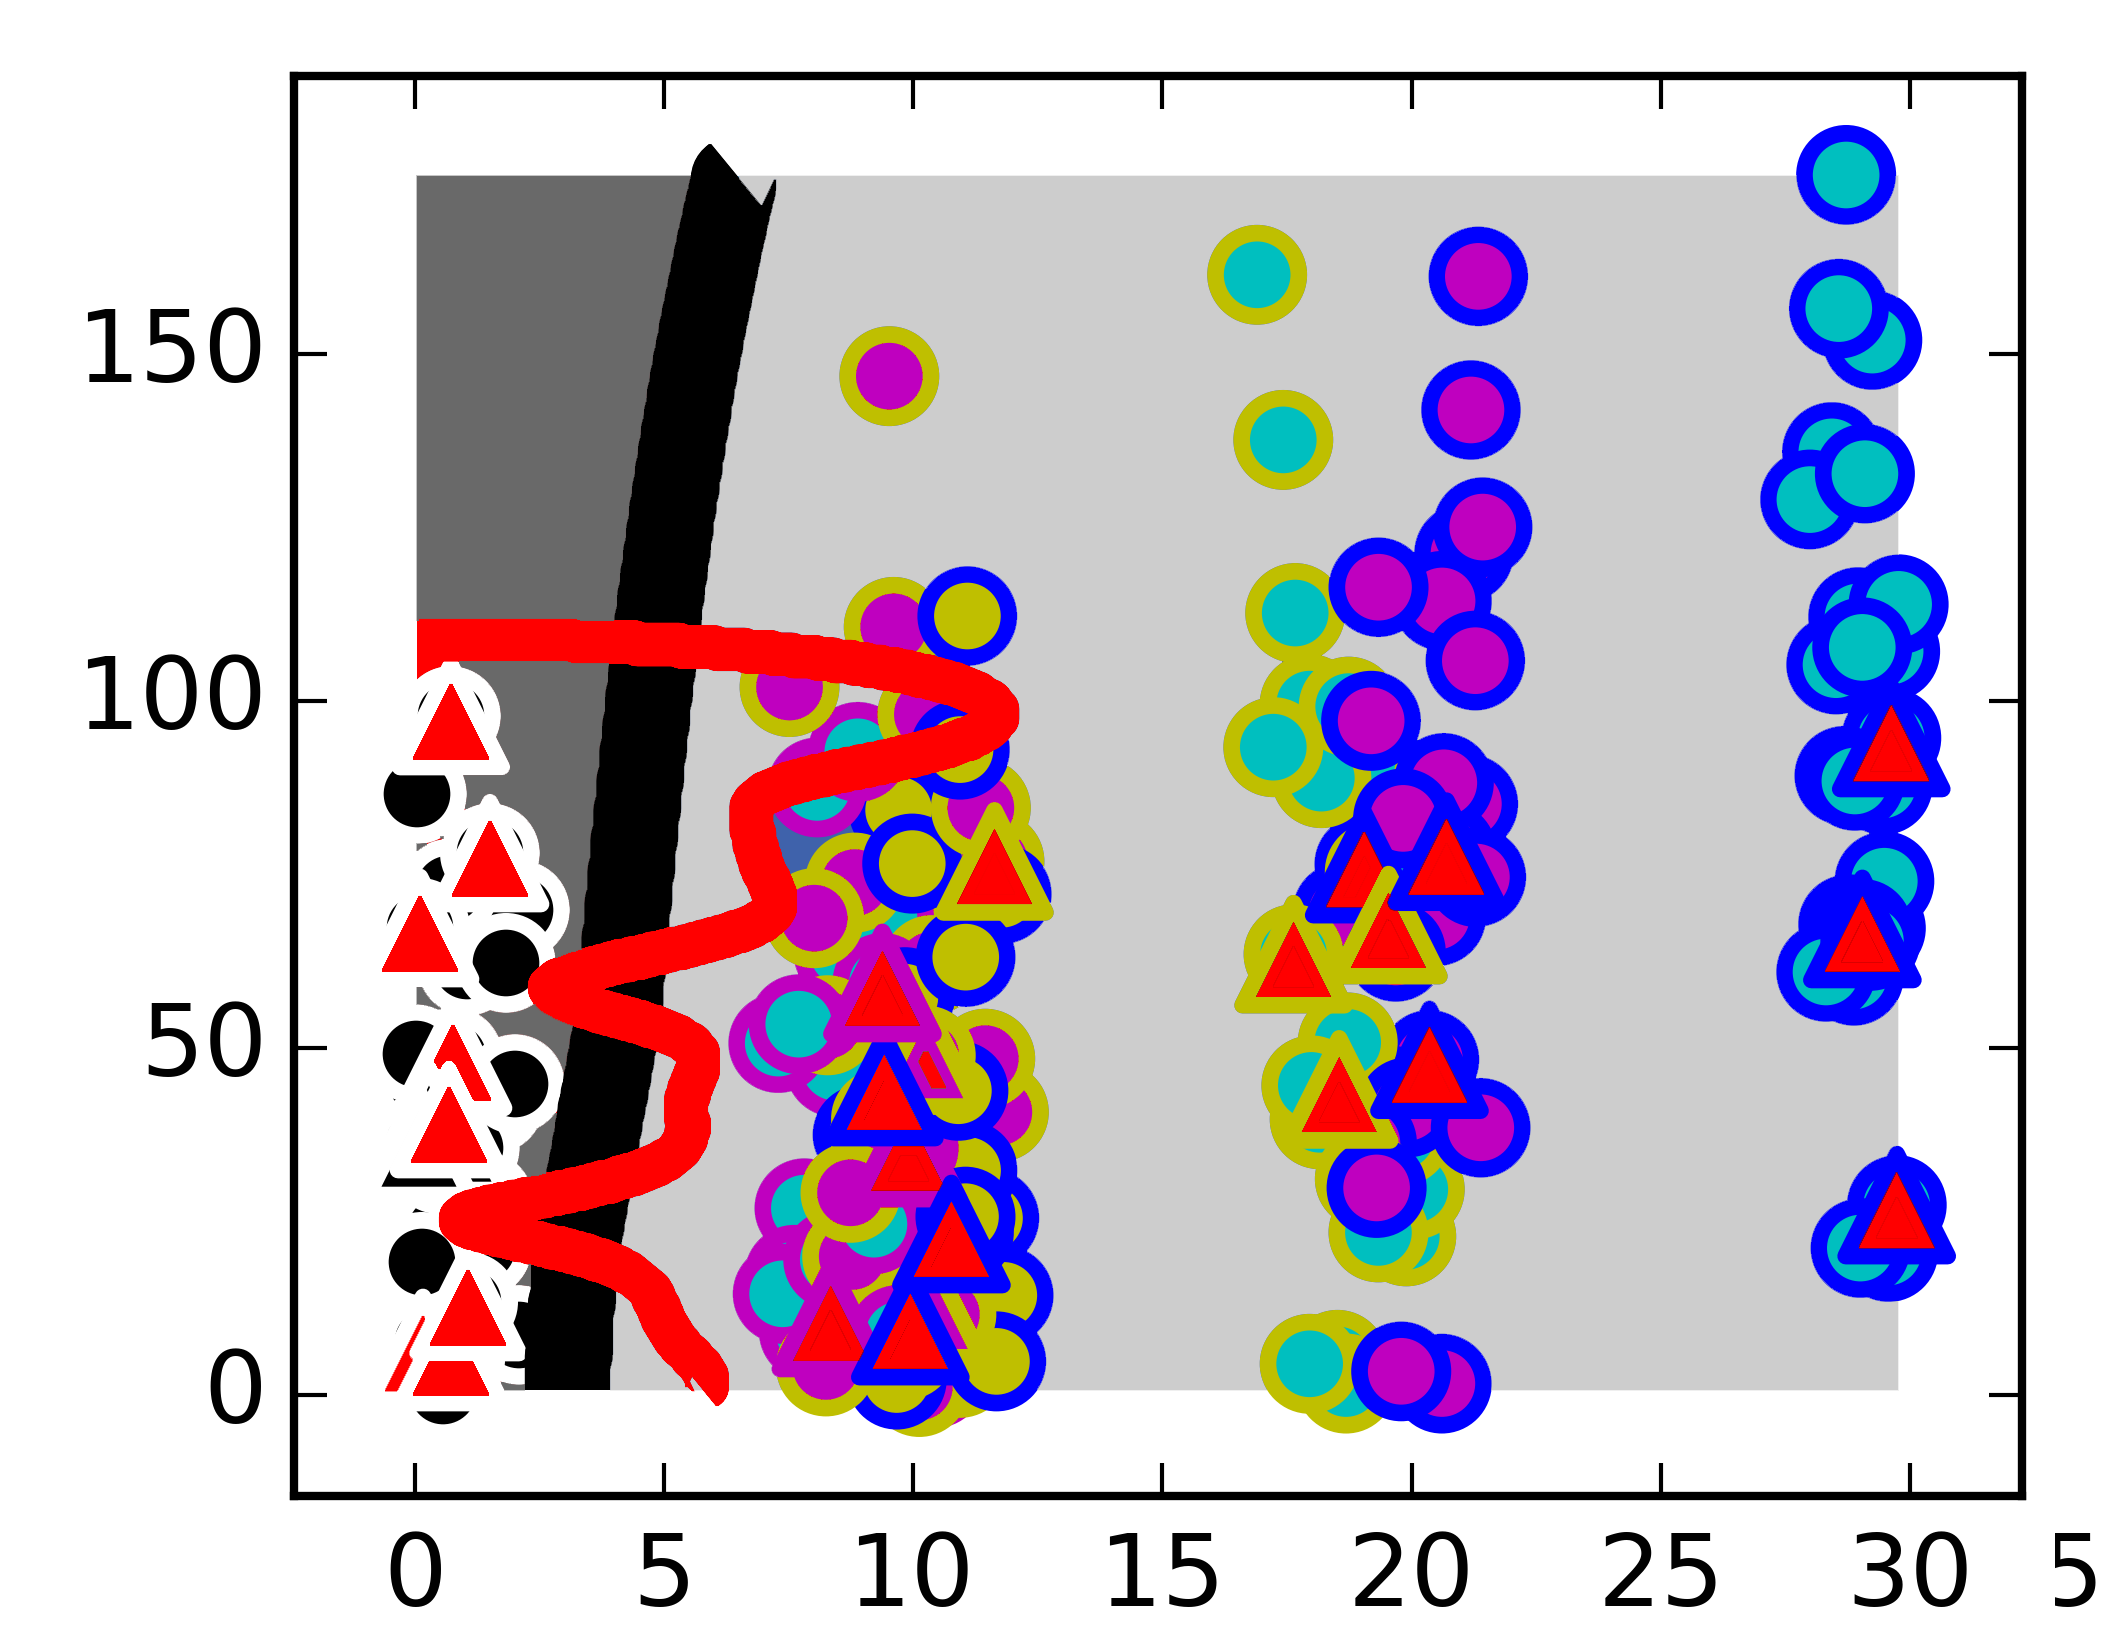
\includegraphics[width=0.25\textwidth]{isosvmproblem2}%
	}
	
	\caption[Motivation for the proposed metric learning approach]{Motivation for the proposed metric learning approach. (a) Example not linearly separable data requiring non-linear metrics. (b) Visualization of the distribution of corresponding absolute pairwise differences (APD), containing the element-wise differences in all dimensions between all possible objects, within (black) and across (coloured) clusters. The background contour shows the probability of a pair with a given distance belonging to the same cluster, learned by Gaussian Discriminant Analysis, and used as the distance pseudometric. Red triangles show the labelled constraints. (c) Example data with non-isotropic variance (three orders of magnitude larger in the y-axis direction). (d) Corresponding APD space coloured as in (a). In addition to the modelled probability of belonging to the same cluster, the models decision boundary (black), as well as the decision boundary of a Support Vector Machine with an isotropic RBF kernel (optimal parameters set by grid search), which overfits along the low-variance dimension.}
	\label{fig:motivation2}
\end{figure*}
 
In contrast, our method sidesteps the difficulty of robustly finding a good non-linear metric for a particular dataset, in a probabilistic framework, without hyperparameter tuning (it has a closed form solution and estimates all parameters from the data). Furthermore, instead of learning a metric using an objective function based on Lp-distance, which collapses the differences along the individual dimensions into one value, it lets the model directly access these individual differences, and thus to learn their importance, allowing it to easily deal with non-isotropic data (Figure \ref{fig:motivation2}c-d). 

Third, it makes explicit the structure in the distribution of constraints. It has been observed before that for data containing clusters, the probability density function of pairwise Lp distances shows two peaks (one for within- and one for across-cluster pairs), e.g. by \citep{brin1995near}. However, in the case of multiple clusters with different shapes and variances, a bimodal distribution is insufficient to reflect the true distributions of the instance differences within or across clusters. Clearly, within-cluster variances in one cluster do not have to equal those in another cluster, and the same is true for across-cluster variances (as illustrated by the variances of the groups of data in APD space in Figure \ref{fig:motivation2}b and d). Learning in pairwise difference vector space (instead of collapsing these distances into scalars) allows our model to adapt locally to within- and across-cluster variances of different clusters, and therefore to better approximate the true pairwise distance distribution. 

\section{Preliminary results}

We use Gaussian Discriminant Analysis (GDA) to learn a data distribution in APD space, and then use this model as a distance function with which to perform clustering, as used to model human spatial representation structure in Chapter 5 (however, note that any probabilistic model could be used in the metric framework introduced in Equation \ref{eq:metric} in Chapters 2.5, not just GDA). To show that the model is not only applicable to human spatial representation data, but also in other domains, we show clustering performance against 5 benchmark datasets used by \citep{zeng2012semi}, and compare it against a recent constrained clustering approach, Constrained Maximum Margin Clustering (CMCC) \citep{zeng2012semi}. 

We evaluate different approaches to perform clustering with the learned distance metric, including the Gaussian Mixture Model (similar to the DP-GMM, but given the correct number of clusters), spectral clustering \citep{ng2002spectral}, weighted, complete, average and Ward agglomerative clustering \citep{mullner2013fastcluster}, and the well-known K-Means clustering algorithm \citep{hartigan1979algorithm}. Figure \ref{mlclust} shows the results.


\begin{figure*}[t]
	\centering
	
	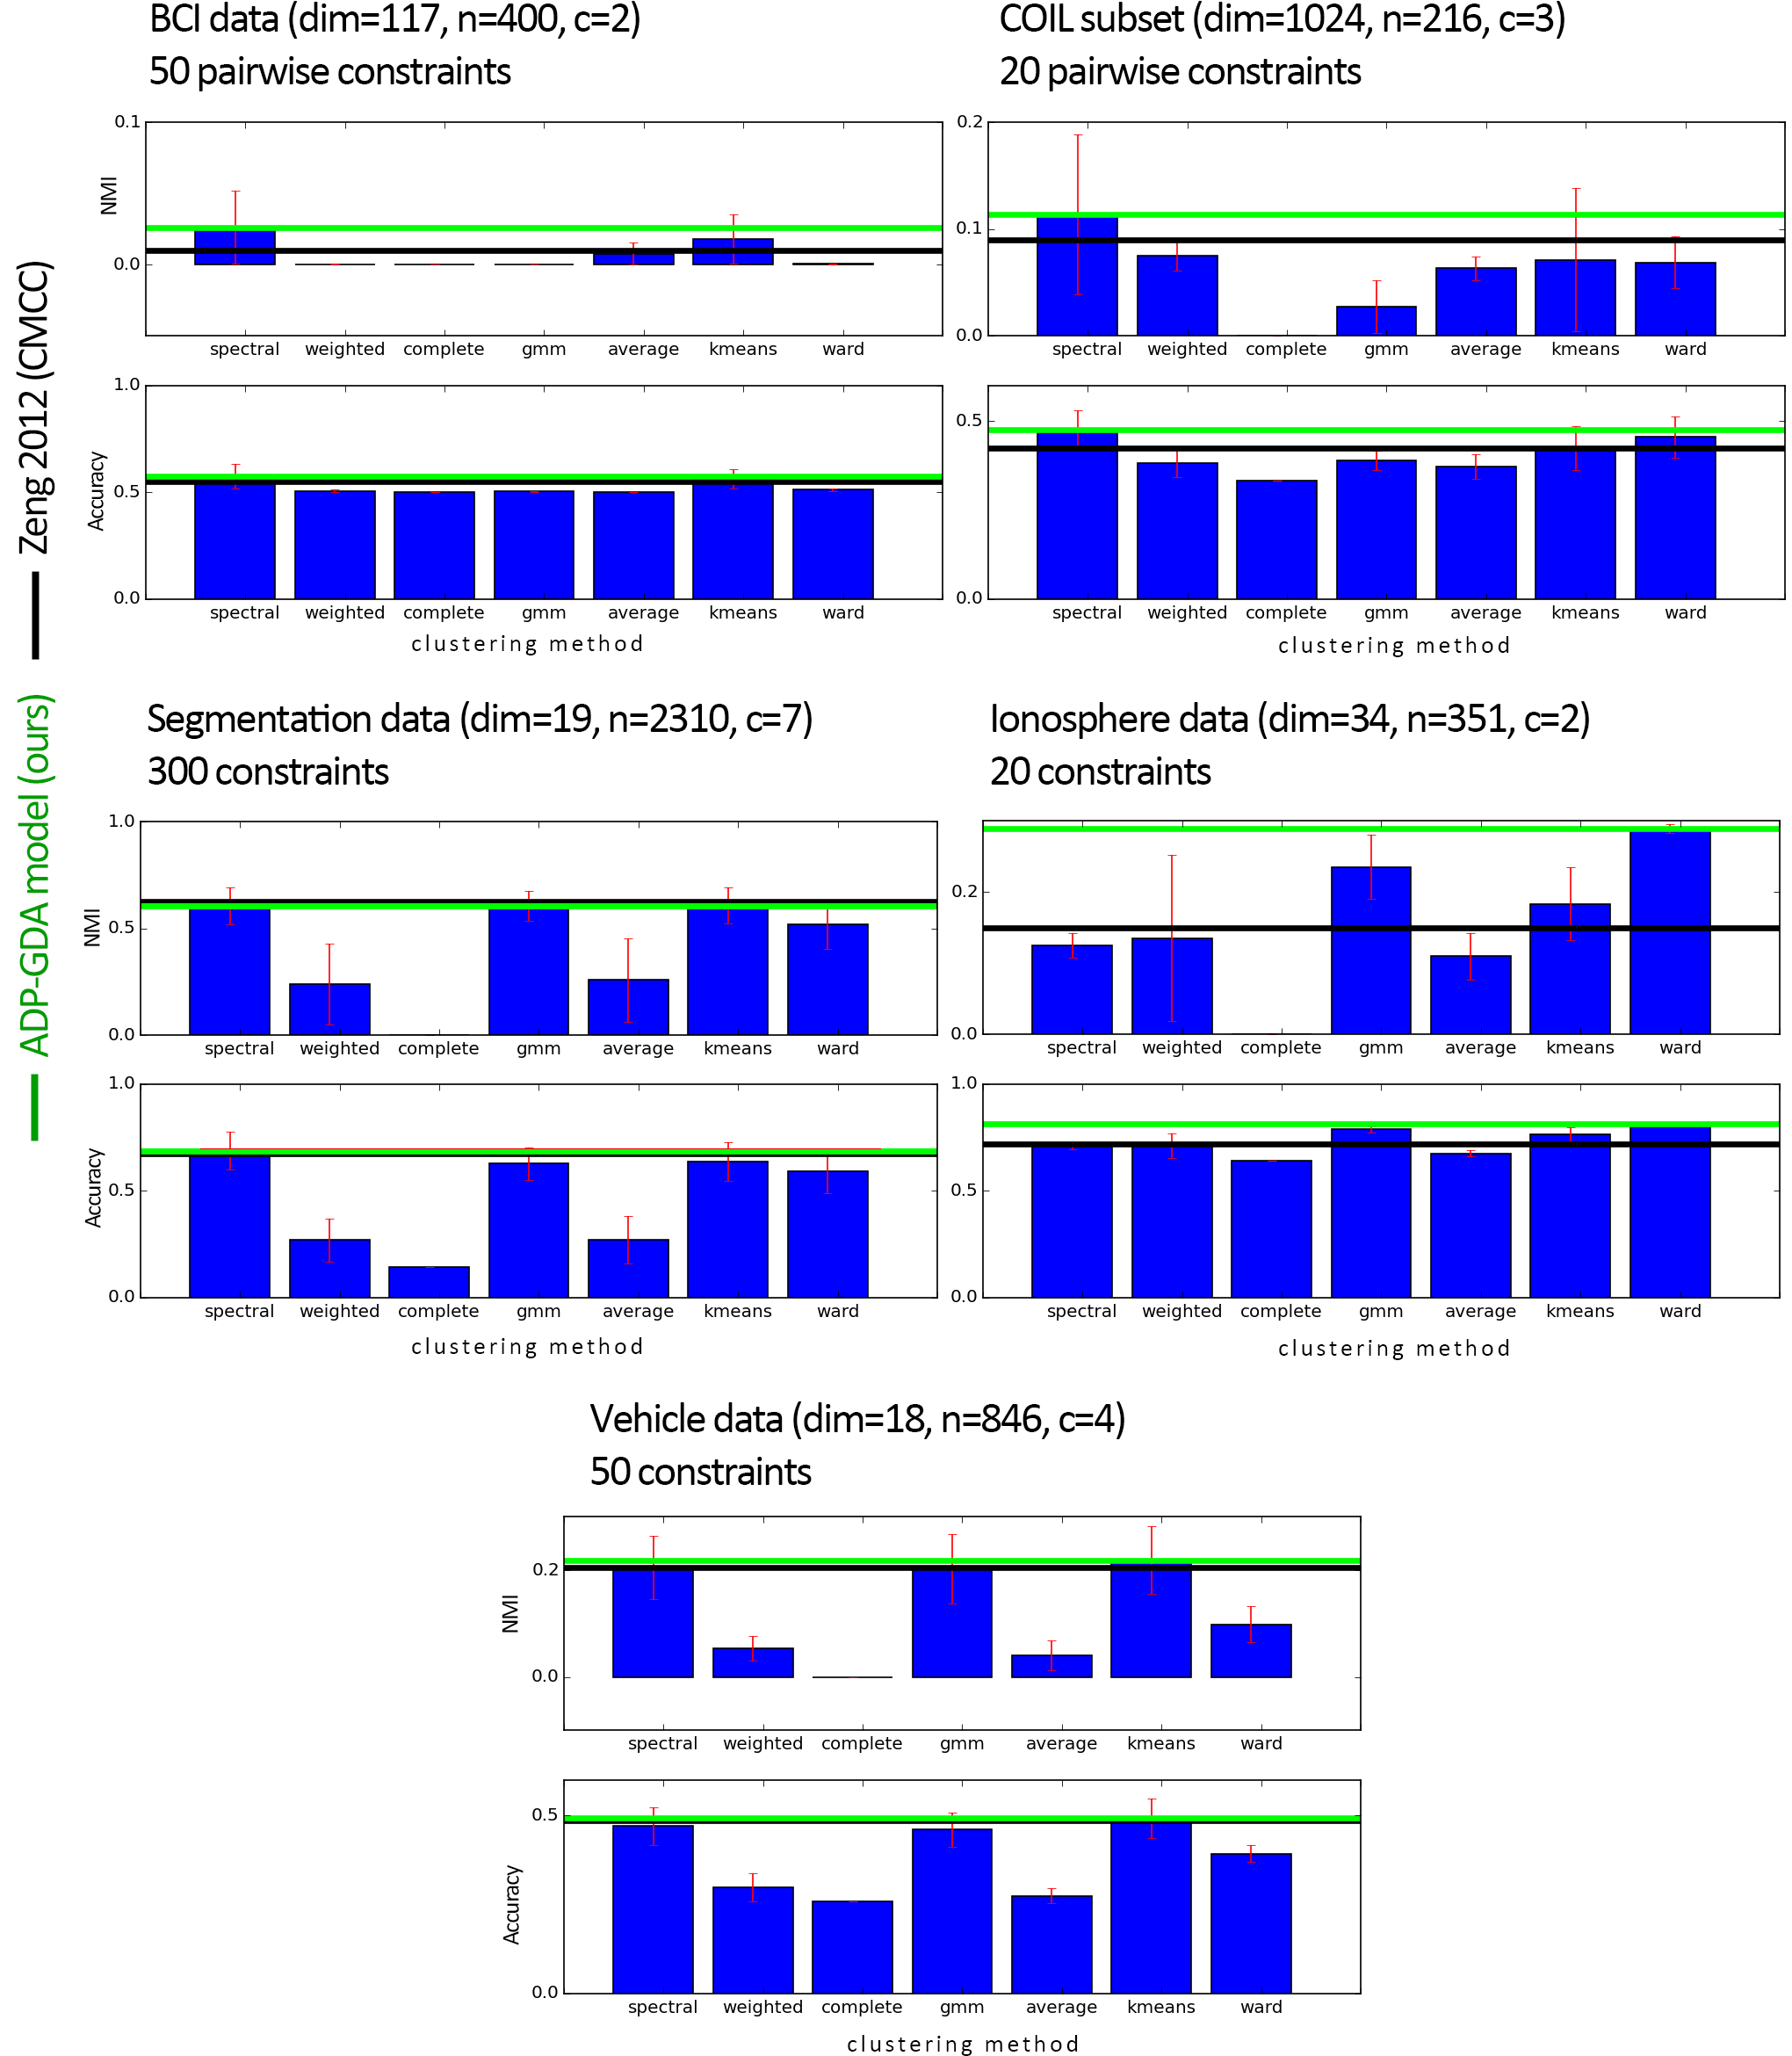
\includegraphics[width=\textwidth]{adsgda_mlresults}%
	
	\caption[Clustering results using the ADS-GDA metric on benchmark datasets]{\textbf{Clustering results using the ADS-GDA metric on benchmark datasets}. Evaluation metrics: NMI (normalized mutual information) and Accuracy (percentage of correctly assigned data points). Abbreviations: dim...dimensionality, n...number of data points, c...clusters.}
	\label{mlclust} 
\end{figure*}




\bibliography{refs}    % this causes the references to be listed

\end{document}
